% !TeX encoding = UTF-8
% !TeX program = xelatex
% !TeX spellcheck = en_US

\documentclass[degree=master]{thuthesis}
  % 学位 degree:
  %   doctor | master | bachelor | postdoc
  % 学位类型 degree-type:
  %   academic(默认)| professional
  % 语言 language
  %   chinese(默认)| english
  % 字体库 fontset
  %   windows | mac | fandol | ubuntu
  % 建议终版使用 Windows 平台的字体编译


% 论文基本配置,加载宏包等全局配置
% !TeX root = ./thuthesis-example.tex

% 论文基本信息配置

\thusetup{
  %******************************
  % 注意:
  %   1. 配置里面不要出现空行
  %   2. 不需要的配置信息可以删除
  %   3. 建议先阅读文档中所有关于选项的说明
  %******************************
  %
  % 输出格式
  %   选择打印版(print)或用于提交的电子版(electronic),前者会插入空白页以便直接双面打印
  %
  output = print,
  %
  % 标题
  %   可使用“\\”命令手动控制换行
  %
  title  = {清华大学学位论文 \LaTeX{} 模板\\使用示例文档 v\version},
  title* = {An Introduction to \LaTeX{} Thesis Template of Tsinghua
            University v\version},
  %
  % 学位
  %   1. 学术型
  %      - 中文
  %        需注明所属的学科门类,例如:
  %        哲学、经济学、法学、教育学、文学、历史学、理学、工学、农学、医学、
  %        军事学、管理学、艺术学
  %      - 英文
  %        博士:Doctor of Philosophy
  %        硕士:
  %          哲学、文学、历史学、法学、教育学、艺术学门类,公共管理学科
  %          填写“Master of Arts“,其它填写“Master of Science”
  %   2. 专业型
  %      直接填写专业学位的名称,例如:
  %      教育博士、工程硕士等
  %      Doctor of Education, Master of Engineering
  %   3. 本科生不需要填写
  %
  degree-name  = {工学硕士},
  degree-name* = {Master of Science},
  %
  % 培养单位
  %   填写所属院系的全名
  %
  department = {计算机科学与技术系},
  %
  % 学科
  %   1. 学术型学位
  %      获得一级学科授权的学科填写一级学科名称,其他填写二级学科名称
  %   2. 工程硕士
  %      工程领域名称
  %   3. 其他专业型学位
  %      不填写此项
  %   4. 本科生填写专业名称,第二学位论文需标注“(第二学位)”
  %
  discipline  = {计算机科学与技术},
  discipline* = {Computer Science and Technology},
  %
  % 姓名
  %
  author  = {薛瑞尼},
  author* = {Xue Ruini},
  %
  % 指导教师
  %   中文姓名和职称之间以英文逗号“,”分开,下同
  %
  supervisor  = {郑纬民, 教授},
  supervisor* = {Professor Zheng Weimin},
  %
  % 副指导教师
  %
  associate-supervisor  = {陈文光, 教授},
  associate-supervisor* = {Professor Chen Wenguang},
  %
  % 联合指导教师
  %
  % co-supervisor  = {某某某, 教授},
  % co-supervisor* = {Professor Mou Moumou},
  %
  % 日期
  %   使用 ISO 格式;默认为当前时间
  %
  % date = {2019-07-07},
  %
  % 是否在中文封面后的空白页生成书脊(默认 false)
  %
  include-spine = false,
  %
  % 密级和年限
  %   秘密, 机密, 绝密
  %
  % secret-level = {秘密},
  % secret-year  = {10},
  %
  % 博士后专有部分
  %
  % clc                = {分类号},
  % udc                = {UDC},
  % id                 = {编号},
  % discipline-level-1 = {计算机科学与技术},  % 流动站(一级学科)名称
  % discipline-level-2 = {系统结构},          % 专业(二级学科)名称
  % start-date         = {2011-07-01},        % 研究工作起始时间
}

% 载入所需的宏包

% 定理类环境宏包
\usepackage{amsthm}
% 也可以使用 ntheorem
% \usepackage[amsmath,thmmarks,hyperref]{ntheorem}

\thusetup{
  %
  % 数学字体
  % math-style = GB,  % GB | ISO | TeX
  math-font  = xits,  % stix | xits | libertinus
}

% 可以使用 nomencl 生成符号和缩略语说明
% \usepackage{nomencl}
% \makenomenclature

% 表格加脚注
\usepackage{threeparttable}

% 表格中支持跨行
\usepackage{multirow}

% 固定宽度的表格。
% \usepackage{tabularx}

% 跨页表格
\usepackage{longtable}

% 算法
\usepackage{algorithm}
\usepackage{algorithmic}

% 量和单位
\usepackage{siunitx}


%自定义usepackage
\usepackage{graphicx}
\usepackage{caption}
\usepackage{subcaption}

% % for pseudocode
% \usepackage{xspace}

% \usepackage{color}
% %% \usepackage[utf8x]{inputenc}
% \usepackage{ulem}
% \usepackage{ctex}

\newcommand{\SA}{$SA$}
\newcommand{\SAM}{{$SA_M$}}
\newcommand{\SAN}{{$SA_N$}}
\newcommand{\SAT}{{$SA_T$}}




% 参考文献使用 BibTeX + natbib 宏包
% 顺序编码制
\usepackage[sort]{natbib}
\bibliographystyle{thuthesis-numeric}

% 著者-出版年制
% \usepackage{natbib}
% \bibliographystyle{thuthesis-author-year}

% 本科生参考文献的著录格式
% \usepackage[sort]{natbib}
% \bibliographystyle{thuthesis-bachelor}

% 参考文献使用 BibLaTeX 宏包
% \usepackage[style=thuthesis-numeric]{biblatex}
% \usepackage[style=thuthesis-author-year]{biblatex}
% \usepackage[style=apa]{biblatex}
% \usepackage[style=mla-new]{biblatex}
% 声明 BibLaTeX 的数据库
% \addbibresource{ref/refs.bib}

% 定义所有的图片文件在 figures 子目录下
\graphicspath{{figs/}}

% 数学命令
\makeatletter
\newcommand\dif{%  % 微分符号
  \mathop{}\!%
  \ifthu@math@style@TeX
    d%
  \else
    \mathrm{d}%
  \fi
}
\makeatother

% hyperref 宏包在最后调用
\usepackage{hyperref}



\begin{document}

% 封面
%% \maketitle

% 学位论文指导小组、公开评阅人和答辩委员会名单
% 本科生不需要
%% % !TeX root = ../thuthesis-example.tex

\begin{committee}[name={学位论文指导小组、公开评阅人和答辩委员会名单}]

  \newcolumntype{C}[1]{@{}>{\centering\arraybackslash}p{#1}}

  \section*{指导小组名单}

  \begin{center}
    \begin{tabular}{C{3cm}C{3cm}C{9cm}@{}}
      李XX & 教授     & 清华大学 \\
      王XX & 副教授   & 清华大学 \\
      张XX & 助理教授 & 清华大学 \\
    \end{tabular}
  \end{center}


  \section*{公开评阅人名单}

  \begin{center}
    \begin{tabular}{C{3cm}C{3cm}C{9cm}@{}}
      刘XX & 教授   & 清华大学                    \\
      陈XX & 副教授 & XXXX大学                    \\
      杨XX & 研究员 & 中国XXXX科学院XXXXXXX研究所 \\
    \end{tabular}
  \end{center}


  \section*{答辩委员会名单}

  \begin{center}
    \begin{tabular}{C{2.75cm}C{2.98cm}C{4.63cm}C{4.63cm}@{}}
      主席 & 赵XX                  & 教授                    & 清华大学       \\
      委员 & 刘XX                  & 教授                    & 清华大学       \\
          & \multirow{2}{*}{杨XX} & \multirow{2}{*}{研究员} & 中国XXXX科学院 \\
          &                       &                         & XXXXXXX研究所  \\
          & 黄XX                  & 教授                    & XXXX大学       \\
          & 周XX                  & 副教授                  & XXXX大学       \\
      秘书 & 吴XX                  & 助理研究员              & 清华大学       \\
    \end{tabular}
  \end{center}

\end{committee}



% 也可以导入 Word 版转的 PDF 文件
% \begin{committee}[file=figures/committee.pdf]
% \end{committee}


% 使用授权的说明
%% \copyrightpage
% 将签字扫描后授权文件 scan-copyright.pdf 替换原始页面
% \copyrightpage[file=scan-copyright.pdf]

\frontmatter
\begin{abstract}
智能体(Agent)是嵌于某特定环境下能够自主行动以实现给定目标的个体。多智能体系统(Multi-Agent System, MAS)通过智能体间的交互实现分布式智能,能够用于解决单个智能体难以或无法解决的问题,是当前人工智能领域的研究热点之一。
%
在当前对智能体的研究中出现多种智能体体系结构和模型,其中Belief-Desire-Intention-based (BDI)智能体模型是当前学术界应用和研究最多的智能体体系结构之一。
%
信念-愿望-意图智能体的关键优势之一是它能够同时追求多个目标。基于Summary-Infomation(SI)的方法、基于Coverage的方法和基于蒙特卡洛树搜索(Monte-Carlo Tree Search)的方法被提出来调度智能体的意图进程以实现并发目标。然而,所有这些现有的工作都局限于调度实现型目标。在实际情况中,智能体可能被要求在一段时间内保持环境状态,而不是实现某些状态。此外,大多数现有的方法也没有考虑到社会准则,如规范norm。他们对智能体意图进行调度的主要目的是为了最大化实现目标的数量,而完全不考虑norm约束。

% 关于本文内容
本文研究了当存在维持型目标和norm约束时调度智能体意图的技术。具体地,本文基于当前基于蒙特卡洛树搜索的调度器\SA,提出一种新的智能体意图调度器\SAM。\SAM 一方面继承\SA 的优势,即高效利用不同意图之间的协同效应,有效避免意图间的相互冲突,另一方面可以在决策时考虑维持型目标或norm以更好地以用户自定义的方式实现目标。本文在火星探测器模拟场景中对\SAM 的性能进行评估,并表明本文的方法在不同困难的一系列场景中优于其他最先进的方法。
\end{abstract}

% 目录
\tableofcontents

% 插图和附表清单
% 本科生的插图索引和表格索引需要移至正文之后、参考文献前
% \listoffiguresandtables  % 插图和附表清单(仅限研究生)
\listoffigures           % 插图清单
%% \listoftables            % 附表清单

% 符号对照表
% % !TeX root = ../thuthesis-example.tex

\begin{denotation}[3cm]
  \item[PI] 聚酰亚胺
  \item[MPI] 聚酰亚胺模型化合物,N-苯基邻苯酰亚胺
  \item[PBI] 聚苯并咪唑
  \item[MPBI] 聚苯并咪唑模型化合物,N-苯基苯并咪唑
  \item[PY] 聚吡咙
  \item[PMDA-BDA] 均苯四酸二酐与联苯四胺合成的聚吡咙薄膜
  \item[MPY] 聚吡咙模型化合物
  \item[As-PPT] 聚苯基不对称三嗪
  \item[MAsPPT] 聚苯基不对称三嗪单模型化合物,3,5,6-三苯基-1,2,4-三嗪
  \item[DMAsPPT] 聚苯基不对称三嗪双模型化合物(水解实验模型化合物)
  \item[S-PPT] 聚苯基对称三嗪
  \item[MSPPT] 聚苯基对称三嗪模型化合物,2,4,6-三苯基-1,3,5-三嗪
  \item[PPQ] 聚苯基喹噁啉
  \item[MPPQ] 聚苯基喹噁啉模型化合物,3,4-二苯基苯并二嗪
  \item[HMPI] 聚酰亚胺模型化合物的质子化产物
  \item[HMPY] 聚吡咙模型化合物的质子化产物
  \item[HMPBI] 聚苯并咪唑模型化合物的质子化产物
  \item[HMAsPPT] 聚苯基不对称三嗪模型化合物的质子化产物
  \item[HMSPPT] 聚苯基对称三嗪模型化合物的质子化产物
  \item[HMPPQ] 聚苯基喹噁啉模型化合物的质子化产物
  \item[PDT] 热分解温度
  \item[HPLC] 高效液相色谱(High Performance Liquid Chromatography)
  \item[HPCE] 高效毛细管电泳色谱(High Performance Capillary lectrophoresis)
  \item[LC-MS] 液相色谱-质谱联用(Liquid chromatography-Mass Spectrum)
  \item[TIC] 总离子浓度(Total Ion Content)
  \item[\textit{ab initio}] 基于第一原理的量子化学计算方法,常称从头算法
  \item[DFT] 密度泛函理论(Density Functional Theory)
  \item[$E_a$] 化学反应的活化能(Activation Energy)
  \item[ZPE] 零点振动能(Zero Vibration Energy)
  \item[PES] 势能面(Potential Energy Surface)
  \item[TS] 过渡态(Transition State)
  \item[TST] 过渡态理论(Transition State Theory)
  \item[$\increment G^\neq$] 活化自由能(Activation Free Energy)
  \item[$\kappa$] 传输系数(Transmission Coefficient)
  \item[IRC] 内禀反应坐标(Intrinsic Reaction Coordinates)
  \item[$\nu_i$] 虚频(Imaginary Frequency)
  \item[ONIOM] 分层算法(Our own N-layered Integrated molecular Orbital and molecular Mechanics)
  \item[SCF] 自洽场(Self-Consistent Field)
  \item[SCRF] 自洽反应场(Self-Consistent Reaction Field)
\end{denotation}



% 也可以使用 nomencl 宏包,需要在导言区
% \usepackage{nomencl}
% \makenomenclature

% 在这里输出符号说明
% \printnomenclature[3cm]

% 在正文中的任意为都可以标题
% \nomenclature{PI}{聚酰亚胺}
% \nomenclature{MPI}{聚酰亚胺模型化合物,N-苯基邻苯酰亚胺}
% \nomenclature{PBI}{聚苯并咪唑}
% \nomenclature{MPBI}{聚苯并咪唑模型化合物,N-苯基苯并咪唑}
% \nomenclature{PY}{聚吡咙}
% \nomenclature{PMDA-BDA}{均苯四酸二酐与联苯四胺合成的聚吡咙薄膜}
% \nomenclature{MPY}{聚吡咙模型化合物}
% \nomenclature{As-PPT}{聚苯基不对称三嗪}
% \nomenclature{MAsPPT}{聚苯基不对称三嗪单模型化合物,3,5,6-三苯基-1,2,4-三嗪}
% \nomenclature{DMAsPPT}{聚苯基不对称三嗪双模型化合物(水解实验模型化合物)}
% \nomenclature{S-PPT}{聚苯基对称三嗪}
% \nomenclature{MSPPT}{聚苯基对称三嗪模型化合物,2,4,6-三苯基-1,3,5-三嗪}
% \nomenclature{PPQ}{聚苯基喹噁啉}
% \nomenclature{MPPQ}{聚苯基喹噁啉模型化合物,3,4-二苯基苯并二嗪}
% \nomenclature{HMPI}{聚酰亚胺模型化合物的质子化产物}
% \nomenclature{HMPY}{聚吡咙模型化合物的质子化产物}
% \nomenclature{HMPBI}{聚苯并咪唑模型化合物的质子化产物}
% \nomenclature{HMAsPPT}{聚苯基不对称三嗪模型化合物的质子化产物}
% \nomenclature{HMSPPT}{聚苯基对称三嗪模型化合物的质子化产物}
% \nomenclature{HMPPQ}{聚苯基喹噁啉模型化合物的质子化产物}
% \nomenclature{PDT}{热分解温度}
% \nomenclature{HPLC}{高效液相色谱(High Performance Liquid Chromatography)}
% \nomenclature{HPCE}{高效毛细管电泳色谱(High Performance Capillary lectrophoresis)}
% \nomenclature{LC-MS}{液相色谱-质谱联用(Liquid chromatography-Mass Spectrum)}
% \nomenclature{TIC}{总离子浓度(Total Ion Content)}
% \nomenclature{\textit{ab initio}}{基于第一原理的量子化学计算方法,常称从头算法}
% \nomenclature{DFT}{密度泛函理论(Density Functional Theory)}
% \nomenclature{$E_a$}{化学反应的活化能(Activation Energy)}
% \nomenclature{ZPE}{零点振动能(Zero Vibration Energy)}
% \nomenclature{PES}{势能面(Potential Energy Surface)}
% \nomenclature{TS}{过渡态(Transition State)}
% \nomenclature{TST}{过渡态理论(Transition State Theory)}
% \nomenclature{$\increment G^\neq$}{活化自由能(Activation Free Energy)}
% \nomenclature{$\kappa$}{传输系数(Transmission Coefficient)}
% \nomenclature{IRC}{内禀反应坐标(Intrinsic Reaction Coordinates)}
% \nomenclature{$\nu_i$}{虚频(Imaginary Frequency)}
% \nomenclature{ONIOM}{分层算法(Our own N-layered Integrated molecular Orbital and molecular Mechanics)}
% \nomenclature{SCF}{自洽场(Self-Consistent Field)}
% \nomenclature{SCRF}{自洽反应场(Self-Consistent Reaction Field)}


% 正文部分
\mainmatter % @WTF: This determines page number form?
\chapter{绪论}
\section{智能体简介}
%智能体
随着近年来人工智能领域的高速发展,计算系统的智能性受到越来越多人的重视。智能体(Agent)是嵌于特定环境中能够自主行动 以实现给定设计目标的个体\cite{DBLP:books/daglib/0023784}。多智能体系统 Multi-Agent System, MAS)\cite{DBLP:books/daglib/0023784}通过智能体间的交互实现分布式智能,能够用于解决单个智能体难以或者无法解决的问题,是当前人工智能领域的 研究热点之一。多智能体相关的研究成果已经广泛应用于工业制造\cite{biernatzki2004agent} 、城市交通等重要领域\cite{DBLP:journals/tits/ChenC10}。

%BDI智能体
在当前针对智能体与多智能体系统的研究中出现了多种用于实现自主智能体的智能体体系结构,包括慎思型结构、反应型结构以 及混合型结构\cite{DBLP:conf/atal/2000, DBLP:journals/ker/WooldridgeJ95}等。
% BDI
其中,基于心理学实践推理(Practical Reasoning)\cite{bratman1987intention}的 Belief-Desire-Intention-based (BDI)模型\cite{DBLP:conf/atal/GeorgeffPPTW98} 是当前学术界应用和研究最多的智能体体系结构之一。
%
采用 BDI模型实现的智能体(BDI 智能体)使用信念(Belief)、愿望 (Desire)以及意图(Intention)等概念来表示自身的心智状态,并通过实践推理来决定下一步应该采取的行动。
%
智能体的信念指的是智能体对其所处环境以及自身的认知,即智能体相信什么;愿望(又被称为目标)指的是智能体想要达到的世界状态的集合。智能 体通过执行计划(Plan)来实现其给定设计目标。计划由 顺序执行的一系列步骤组成。每个步骤是能够改变当前世界状 态的基本动作,或者是需要由智能体实现的子目标。
%
当智能体选择 某一特定计划来实现其给定目标时,该计划未执行的部分被称为实 现该目标的意图,即智能体承诺为了实现目标而执行的步骤。

到目前为止已有许多基于BDI智能体架构的编程语言和平台被提出并广泛应用。最早基于BDI架构的智能体系统是Procedure Reasoning Systems(PRS),其被开发用于航空领域\cite{DBLP:conf/aaai/GeorgeffL87}以及网络交通领域\cite{DBLP:conf/aaaiss/Wobcke07}。AgentSpeak(L)\cite{DBLP:conf/maamaw/Rao96},一种抽象的BDI智能体编程语言,主要目的是帮助人们理解BDI架构在实际中的应用(例如PRS)与BDI架构理论模型直接的关系。Jason\cite{bordini2007programming}是一门基于AgentSpeak(L)开发的实用性语言,其语言的底层实现基于JAVA,有着很好的跨平台特性。除此以外,还有许多其他基于BDI架构的语言和平台,例如2APL\cite{DBLP:journals/aamas/Dastani08},3APL\cite{DBLP:books/sp/map2005/DastaniRM05}以及JACK\cite{DBLP:books/sp/map2005/Winikoff05}。

目标与意图是BDI智能体的核心。在 BDI 模型中,一个目标通 常对应有多个不同的实施计划以应对不同的环境状态。智能体需要 选择执行其中的一个计划来实现其自身目标。该问题被称为 BDI 智 能体的计划选择(Plan Selection)问题\cite{yao2017robust}。在许多实际问题中, BDI 智能体都会被同时赋予多个目标进而产生多个并行意图。此 时,BDI 智能体需要决定下一步应该执行哪一个意图。该问题被称 为 BDI 智能体的意图选择(Intention Selection)问题\cite{yao2017robust}。在\cite{DBLP:conf/emas/Castle-GreenDL20}中,智能体的计划选择与意图选择被称为智能体慎思过程中的意图 进展问题(Intention Progression Problem, IPP),即 BDI 智能 体在每一个慎思周期中都需要选择其下一步需要执行的意图,如果 被选择的意图的下一步是子目标,那么BDI智能体还需要选择实现目标所需要的计划。


IPP是BDI智能体研究中的一个关键问题,任意地进行意图进 展可能会导致不同意图间的冲突,例如,智能体$\alpha$有两个目标:前往地点A和购买电池;前往地点A可由两个计划实现:行走前往和打车前往。若$\alpha$先选择打车前往 A,则可能由于打车的资金花费而导致后续没钱购买电池,而选择行走前往则不会造成该冲突。

\section{国内外研究现状}
本节对现有相关研究进行文献述评,分别考虑了对经典意图进展问题的相关研究,对维持型目标的相关研究以及norm约束下决策问题的相关研究。
% 考虑分三点:1.传统意图进展问题,2.norm约束下的决策,3.维持型目标下的决策
\subsection{经典意图进展问题研究现状}
% SI
在对意图进展问题的研究中,Thangarajah等人\cite{DBLP:journals/jar/ThangarajahP11,DBLP:conf/ijcai/ThangarajahPW03}提出了基于SI (Summary Information)的意图调度算法,其通过自底向上总结信息的方式确定实现目标的必要条件、可能条件、必要结果以及可能结果来推理出意图之间是否存在冲突以及是否存在协同效应。SI算法在智能体程序编译期进行信息总结计算,并在运行期间随着智能体意图的进展动态更新总结信息。此外,SI支持实时判断接收新目标的机制,允许智能体在运行时根据总结信息判断新的目标是否一定会、可能会或一定不会与当前目标相冲突,然后决定是否接收新的目标。然而,该方法假设现有目标的优先级总是大于新目标,若发生冲突则不接收新目标,而不会考虑抛弃现有的冲突目标。

% C
Waters等人\cite{DBLP:conf/atal/WatersPS14,DBLP:conf/aamas/ThangarajahSP12}提出了CB(Coverage Based)意图调度算法,并在后续研究中对其进行了改进\cite{DBLP:journals/aamas/WatersPS15}。CB考虑在编译期对实 现目标计划的健壮性进行数值化刻画,提出在不同环境下智能体实 现某个目标的可执行性(Coverage),以及在同一环境下智能体实现 某个目标的计划选择多样性(Overlap)。在意图进展过程中CB优先考虑实现脆弱的目标,以免因为环境自身的动态性导致目标因无可选计划执行而无法实现。相较于SI,CB重点考虑的是智能体在动态环境下的意图进展。

% MCTS
Yao等人提出了基于蒙特卡洛树搜索(Monte Carlo Tree Search,MCTS)的意图调度算法\cite{DBLP:conf/aaai/YaoLT16,DBLP:conf/atal/YaoL16,DBLP:conf/ecai/YaoLT14,DBLP:conf/atal/Yao21,DBLP:conf/ijcai/Yao20,DBLP:conf/ecai/YaoLT16},其利用MCTS的特点,专注于对最有前景的行为进行搜索,并基于随机模拟构建并不断扩展搜索树,最终根据用户自定义的评判标准和搜索树记录信息得到决策结果。和SI以及CB不同,MCTS算法的执行发生在程序运行期,其总是基于当前状态对决策空间进行搜索,并得出当前决策结果。MCTS调度策略被应用于消 解并行意图间的冲突、开发并行意图交错执行的协同效应、对时间 限制的意图进行调度以及在动态和不确定环境下的意图调度。此外,根据对目前该研究领域的调研,得知基于MCTS的意图调度算法 是当前可验证的最好的意图调度策略。
% 传统意图调度方法的问题
然而,上述方法都没有考虑到社会模拟场景中维持型目标对智能体的影响,缺乏在意图调度是考虑维持型目标的能力。


\subsection{维持型目标研究现状}
虽然 BDI 智能体在多个领域得到广泛应用,但是在智能体目标的表示与推理机制方面,以往相关研究大多聚焦于实现型目 标,而没有考虑到维持型目标。维持型目标定义了一些情况下以维 持某个状态一段时间为目标,例如火星探测器需要在勘探过程中维 持电量在某一数值之上,以确保其能够在勘探之后顺利返回基地补 充电量。Dastani等人\cite{DBLP:conf/atal/DastaniRM06} 描述了维持型目标,刻画了智能体对维持某 一个状态需求的基本模型。然而,现有意图调度算法大多仅考虑了实现型目标,即到达某个世界状态,而没有考虑维持某个世界状态 的维持型目标。目前仅有的对维持型目标加入考虑的意图调度算法\cite{DBLP:conf/atal/DuffHT06,DBLP:journals/ci/DuffTH14,DBLP:conf/dalt/HindriksR07}并没有考虑到多意图并行交错执行对维持型目标的影响。

% maintanance goal
在对维持型目标的研究中,Duff等人提出一种基于SI的意图调度算法\cite{DBLP:conf/atal/DuffHT06},其在决策过程中加入对维持型目标的考虑:若实现型目标将与维持型目标冲突,执行预防措施(例如补充资源)。 然而,和SI类似,该算法假设当前的目标优先级总是高于新的目标,并且如果新的目标为维持型目标且与当前目标相冲突,维持型目标将被直接抛弃。后来Duff等人在\cite{DBLP:journals/ci/DuffTH14}中拓展了维持型目标的规范语法及语义,但是意图调度策略并没有被改进。Hindriks等人\cite{DBLP:conf/dalt/HindriksR07}提出了一种处理维持型目标的决策机制,该机制直接避免执行破坏维持型目标的行动,保证维持型目标不会被破坏。然而该方法将会导致智能体可执行的行动变少,降低智能体的灵活性。Thangarajah等人\cite{DBLP:conf/ecai/ThangarajahHMY14}分析了维持型目标的进展过程,提供了一套合理的维持型目标进展模型,但是起没有考虑到意图进展问题。

目前在BDI智能体研究领域中,已有多种对智能体的功能性进行拓展的方法被提出以提升其适用性。鉴于大多数对智能体目标的研究 都着重关注实现型目标和维持型目标,Dastani等人\cite{DBLP:conf/atal/DastaniRW11}提出以时序逻辑来表示目标,以拓展智能体支持的目标种类。在他们提出的框架中,目标的表示不仅包含基本命题,还包含时序连接符号如$\diamond$(最终),$\square$(总是)以及$U$(直到)。在具体应用时,由于大多数智能体语言和平台都不支持时序逻辑,需要将时序逻辑表示的目标转化为一般化的实现型目标和维持型目标以便用于实际使用。Dastani等人提出操作化(Operationalization)方式,根据时序连接符不同,对时序逻辑表示的目标进行合理转化,使其转变为一个或多个逻辑对应的实现型目标和维持型目标。然而,该框架并没有提供一个一般性的意图调度算法,某些特殊形式的目标仍然需要用户自定义条件-动作对,虽然有一点的拓展性,但加重了用户的负担;此外,该框架也没有考虑到社会仿真场景下的norm,这导致其不适用于norm约束场景。
\subsection{Norm约束下的决策问题研究现状}
% 社会模拟场景
BDI智能体在社会模拟场景中也有广泛的应用\cite{DBLP:conf/ijcai/SinghSPJ11},其类人的内部心智状态表示以及行为推理方式使其能够灵活地适应于多种社会模拟场景。BDI智能体程序自然假设环境是动态的,能够在不同情 况下实时选择合适的方式实现目标;另外,BDI 智能体有能力处理执行失败的情况,当某个计划执行失败时,其可以通过失败恢复机 制重新考虑如何实现当前目标。此思考与运行机制使得BDI智能体拥有高度适应性与灵活性,并且与人类操作方式非常类似,这使其有能够合理应用于社会模拟场景。

% Norm
在一些社会模拟场景中,环境是开放的,不同类型的智能体可以随意地选择离开或是加入,它们的行为能力与目标也不尽相同。这些特性使得开放多智能体系统的运行状况与结果难以预测与控制。当一些智能体实施恶意行为时,其会对其它正常运行的智 能体甚至整个系统造成严重损害。为了保证环境的可控性与稳定性,norm的概念被提出作为管控智能体行为的一种方式\cite{DBLP:journals/mags/SavarimuthuC11},其对智能体的行为在一定条件下加以特定约束,用于确保智能体 在环境中的合理、合规地运作。norm 通常定义了系统中智能体‘道义’方面的行为准则。Norm 以义务(Obligation)来规范智能体在 某些情景下应该去做什么,例如在超市里,智能体应该付完钱之后再带着商品离开;norm以许可(Permission)来规范智能体在特定 场景下可以做什么,例如智能体在环境中移动是被许可的;norm也可以禁令(Prohibition)来规范智能体在特定场景下不能去做什么,例如在开放多智能体系统中攻击或伤害其它智能体是被禁止的。Norm对智能体的约束可能会对智能体实现目标的过程造成阻碍,或是限制智能体某些特定的实现目标的方式。盲目的、不考虑 norm的智能体运行机制势必会导致低效的执行效果。例如,当一个智能体正常前往某个目的地需要过马路时,它需要考虑交通规范norm对其的约束:在红灯时不能过马路(即使它有能力这么做,否则,将受到罚款。另一方面,若智能体需要尽快到达目的地时(例如救火),其可以考虑违反交通规范norm,优先实现更为重要的目标,若智能体没有考虑norm对其实现目标的影响的能力,则无法做出合理的决策。因此,一个高效的、能够对 norm进行合理考虑的智能体意图调度机制对构建适应性强、运行在norm作用环境下的智能体有十分重要的意义。
规范实践推理(Normative Practical Reasoning,NPR)指的是智能体在实践推理的过程中考虑norm对其影响。在其相关研究领域中,研究者们提出了多种考虑norm的智能体决策方法。

% norm决策
% BOID
对NPR的研究最早或许可以追溯到BOID架构\cite{DBLP:conf/agents/BroersenDHHT01},BOID架构实质上是对BDI架构的一种延申,赋予其决策时考虑norm的能力。BOID在BDI的基础上引入了智能体性格类型的概念以处理norm与行动、目标之间的冲突。BOID智能体可以是社会型的、无视规范型的等,不同类型的BOID智能体对norm有不同的解释,在解决norm相关冲突时也有不同的策略。例如无视规范型的智能体会更倾向于考虑自身目标的实现,而不过多考虑norm对其约束,在norm相关冲突发生时忽略norm的存在。BOID智能体的决策过程是纯粹基于命题规则的。如果在其决策过程中某些规则发生冲突(可能由norm造成),智能体将基于其自身类型进行冲突消解以得到最早确定的决策结果。BOID架构的设计非常简洁,易于理解,但是这种架构并没有广泛的实际应用。很大 一部分原因在于其健壮性低下,仅依靠逻辑推理做出决策,决策过程的时间复杂度高,当规则量庞大时,极其耗时,且不易维护。

% NoA
NoA\cite{DBLP:conf/ijcai/KollingbaumN03}架构基于BDI架构并引入了norm的相关概念,例如义务,禁令以及许可。许可规范了智能体可以做什么(而不一定要去做)。在决策阶段,NoA架构规范了智能体该从计划库中选择哪个计划去执行以遵守norm的相关约束。NoA是完全以norm为主导的架构,它没有自身内部的目标,因此不需要考虑norm与目标的冲突。这使得NoA总是会做出遵守norm的行动。NoA能够处理norm的相关概念,其架构设计也较为简易,易于理解。然而--中仅使用文字对NoA的概括性描述,而缺乏对NoA架构抽象准确的形式化定义。没有内部状态,完全以norm为导向的设计也使得NoA架构适用场景受限,限制了BDI智能体的基本自主性。


基于norm的行为修改(Norm-based Behavior Modification,NBM)\cite{DBLP:conf/atal/MeneguzziL09}是对基础BDI架构的一种延伸,其解决的问题主要是智能体在运行时如何去适应新的norm,NBM架构的重点在于提供一种机制使得智能体有能力在运行时去约束一些计划的执行以适应其在运行时所检测到的新的norm。其优点在于其方法依然在BDI的框架下,对于新的norm,创建一个新的计划来处理,将那些norm禁止的计划进行限制,不让其在后续norm生效的情况下执行。该机制可以方便地部署到其它符合BDI架构的智能体系统中。虽然本文实现了在运行时应对新检测的norm的机制,但是没有对norm对于智能体的影响进行精确地刻画,简单认为norm禁止的计划就不能去执行,使得智能体灵活性降低。其研究重点关注的问题也仅限于计划选择,目标选择并不在其考虑范围之内。

% N-2APL
N-2APL\cite{DBLP:conf/aamas/AlechinaDL12}是基于2APL\cite{DBLP:journals/aamas/Dastani08}的智能体编程语言。 N-2APL在2APL的基础上拓展了对norm的表示与处理机制,支持表示义务、禁令等概念,支持在决策过程中处理norm带来的冲突。N-2APL的目标选择与计划选择机制是基于实现目标截止期限以及计划优先级制定的。N-2APL假设计划优先级由编程人员根据norm的影响提前定义。其决策过程主要为: 1.放弃某些低优先级的目标以确保高优先级的目标能够在截至期限内完成;2.选取一个高优先级且能够在截止期限实现的目标;3.根据提前定义好的优先级顺序选择计划执行。
在N-2APL中,有限制条件的义务并没有被考虑,使其应用场景受限。N-2APL通过引入原子计划与非原子计划的概念,以降低可能的执行序列的数量来控制决策算法的时间复杂度并消解计划间并行执行的冲突:原子计划执行时不能被打断,而非原子计划执行过程中可以被其他计划打断。这种设计需要编程人员手动对计划进行分类,不利于大规模实践应用;由于可能执行序列的减少,这种设计也会一定程度上降低了BDI智能体的灵活性。

% N-Jason
N-Jason\cite{DBLP:conf/dalt/LeePLDA14}是一个基于Jason\cite{bordini2007programming}智能体编程语言,支持运行时处理未知norm智能体编程语言。相较于以往的norm处理机制——假设norm在运行前就已经确定,在运行时也不会改变, N-Jason支持运行时对未知norm的识别。如果N-Jason识别到义务norm,则将其转化为一个新的目标待后续阶段实现;如果识别到禁令norm,则将其加入禁令norm集合,供后续进行冲突消解阶段应用。与N-2APL类似,N-Jason 也支持基于截止期限与norm的影响对目标、 计划划分优先级以消解冲突并选择合适的计划执行。然而,不像N-2APL,N-Jason没有考虑多目标之间的选择问题,仅考虑了如何选择计划。作者也提到基于N-Jason产生的的智能体行为可能在编程人员看起来是不可解释、不可预测的,然而却没有提供确切的理论或实践依据。

% v-BDI
v-BDI\cite{DBLP:journals/eaai/MeneguzziROVL15}对BDI架构进行了拓展,在决策时加入了对norm的考虑,其允许智能体在norm冲突发生时,根据自身认识自主地选择是否遵守norm,v-BDI的关键技术在于在计划选择时先对各计划的行动进行模拟运行,然后根据模拟结果对比各个计划的价值,最终选择出价值最大的计划执行。v-BDI依据计划价值来进行计划选择, 当执行计划的收益大于违反norm受到的惩罚时,智能体可以选择去做出违反norm的行为以获得更大的整体收益。这种机制保留了BDI智能体的灵活性与自主性,同时计划选择的标准由模拟结果决定, 不需要编程人员明确给的。编程人员仅需要定义模拟的价值函数即可。v-BDI中对计划价值的计算仅考虑其中的行动,而不考虑子目标,这使得价值计算过程的时间复杂度较低,易于实际的应用。然而v-BDI仅考虑到了计划选择问题,而并没有提及多目标情况下的目标选择问题。仅考虑计划中行动的模拟机制虽然高效,但是必然会因为没有考虑到子目标而导致价值计算不准确。

此外,在非BDI架构领域,也有一些对norm考虑的决策机制被提出。相较于BDI架构,非BDI架构的智能体没有事先由编程人员定义好的计划库,而仅有由一个个独立的行动组成的行动集合。因此,设计非BDI架构智能体norm决策机制最大的挑战在于如何在norm规范下根据一定的规则,基于行动集合生成某些执行序列以供智能体执行,达到设计者的设计目标。

%
Shams等人\cite{DBLP:conf/atal/ShamsVPV15}提出的方法使用到了提前设定好的计划,但是其和BDI智能体的差异在于Shams等人提出的决策过程允许智能体根据norm的影响动态调整执行计划。其在运行时选择执行序列并将其与当前计划相比较,若新执行序列组成的计划的收益大于当前计划,则将新生成计划作为当前计划执行。Norm对智能体行为的约束体现在若智能体做出违反norm的行为将受到一定数值的惩罚。各行动受惩罚值的大小决定了智能体会如何执行计划:智能体总是会执行整体收益(实现目标的收益+违反norm的惩罚)最大的计划。该方法能够通过搜索得到最优的计 划,但是其时间复杂度较高,若可选计划数量较多,则实际应用较为困难;同时其也没有考虑到多个并行执行的计划之间的相互冲突与影响。

% RL
Li等人\cite{DBLP:conf/atal/LiMFL15}提出了使用强化学习方法对变化的或位置的norm进行学习,并根据学习结果对智能体自身的行为进行动态调整,以更好地在norm存在的环境中实现目标。Li等人\cite{DBLP:conf/atal/LiMFL15}分别对两种强化学习方法 Q-Learning 和 SARSA\cite{Sutton2005ReinforcementLA}进行了测试,验证了其有效性并对比分析了 两种方法的特点与适用场景:Q-Learning更加激进,对norm的学习的速度很快,但是不太稳定;SARSA比较保守,对 norm的学习速度慢,但是稳定性高。与—类似,\cite{DBLP:conf/atal/LiMFL15}没有考虑多目标之间的冲突问题,并且当问题规模较大时,这两种基础强化学习方法需要消耗大量计算时间,不利于实际应用。

% argumentation based
Shams等人\cite{DBLP:conf/ijcai/ShamsVOP16,DBLP:journals/taas/ShamsVOP20,DBLP:conf/atal/ShamsVPV15}提出的方法在不同场景设定下对 norm 的考虑主要体 现在可解释性,其实用 Argumentation Dialog 的方法试图对智能体 在 norm 约束下的行为进行解释,以提高人类对智能体程序的信任 度。同时,其考虑到了 norm 与智能体目标之间的冲突问题,提供了 一套消解冲突的机制。然而,与\cite{DBLP:conf/atal/LiMFL15}类似,在各个场景下该机制的 时间复杂度较高,并且没有考虑多个目标之间的冲突。


综上,目前对智能体在维持型目标的支持、norm约束下的决策以及对智能体目标种类的拓展方面的研究都取得了重要的进展。然而现有研究依然存在一些问题与空白。

现有的BDI模型不支持维持型目标,且目前对维持型目标研究也仅仅考虑单个目标的执行对维持型目标的影响,而没有考虑多目标并行执行的情况,因此无法有效解决引入维持型目标带来的问题。

现有的BDI慎思过程框架缺乏对norm的支持,使得智能体在决策时无法考虑到norm对其行为的约束作用,进而无法做出合理的决策;同时,现有的对BDI智能体意图调度的相关研究也并没有考虑到norm对智能体的影响,使得其无法用于解决norm约束下智能体意图调度问题。

现有的相关研究大多仅针对社会仿真场景下的某一方面的问题(例如仅针对norm或维持型目标),而没有考虑norm和维持型目标共存的情况,缺乏一般性。
在真实社会场景中,复杂多变的环境往往需要智能体有更强的功能性与灵活性,例如要求智能体同时处理各种类型的目标以及norm。然而现有研究大多都仅针对解决某一特定的需求或增强某一特定的功能,在维持型目标的研究中没有考虑到norm的影响,另一方面在norm的相关研究中没有考虑到其他更加复杂种类的目标。这种现状一定程度上限制了BDI智能体的一般性与通用性。

\section{立题依据}
% 问题
根据上述对研究背景和意义的介绍与分析,得知当前在BDI智能体决策研究领域有如下问题:
\begin{enumerate}
  \item 现有关于智能体决策的研究大多针对实现型目标,而极少考虑到维持型目标,特别是实现型和维持型目标共存的情况。另一方面,在针对维持型目标的研究中没有考虑到多意图并发执行的问题。
  \item 现有的关于NPR研究中没有考虑到多意图并发执行的情况,意图之间的交错执行与相互影响被忽略。这使得智能体无法在norm约束下高效实现多个目标。另一方面,大多现有的关于多意图调度算法中没有考虑到norm对智能体的影响。
  \item 维持型目标与norm共存的情况再模拟社会场景中并不少见,然而现有研究大多仅针对解决一个方面的问题(或维持型目标或norm),缺乏一般性。
\end{enumerate}

%
为了解决上述问题,本文充分研究了社会仿真模拟场景下智能体的行为决策相关技术,并基于随机采样模拟和时序逻辑提出一系列BDI智能体意图调度方法:
\begin{itemize}
  \item
针对问题1:本文将研究并实现对维持型目标全面支持的智能体意图调度方法,该方法在SA的基础上进行拓展,在决策时加入对维持型目标的考虑,使得智能体能够在意图调度过程中考虑到维持型目标,拓展智能体的适用领域。根据智能体对环境的确定性不同,该方法考虑了主动的维持型目标(在维持型目标被破坏之前尝试修复操作)以及被动的维持型目标(在维持型目标被破坏之后尝试修复操作),以适应不同的应用场景。
  \item
针对问题2:为了实现 norm 约束下的意图调度算法,本文将对智能体的norm约束问题模型,多目标交错执行触发 norm 问题以及 norm 对智能体决策的影响问题展开研究,提出norm约束下的意图决策方法,该方法在SA算法的基础上进行拓展,对其运行时的多个阶段进行拓展,加入对norm的考虑,实现智能体高效地在 norm 约束环境中并行实现多目标能力,提高智能体的适用性。
  \item
针对问题3:本文在对前两个问题的研究基础之上,提出基于时序逻辑(Linear Temporal Logic,LTL)的意图调度算法,使得智能体可以同时处理norm与维持型目标。此外,由于时序逻辑的一般性,使得该方法有较强的拓展性,其可适用范围不限于norm与维持型目标,而可被应用于用户自定义类型的目标(例如条件限制的维持型目标或实现型目标)或是其他场景约束。
\end{itemize}
%
\section{论文主要内容及章节安排}
本文的章节安排如下。第二章首先介绍智能体的基本背景概念,再引出一种热门的智能体架构-BDI智能体架构;然后对现有相关研究内容进行文献述评,分析不同研究所提出方法的特点以及局限性。

第三章中首先对BDI智能体的相关概念如信念、意图等进行规范定义,并介绍使用目标计划树的数据结构表示智能体意图的方法;然后,基于目标计划树模型对研究问题,即意图进展问题进行规范形式化定义。

第四章介绍本研究所基于的核心算法蒙特卡洛树搜索(Monte-Carlo Tree Search,MCTS)。并对其算法进行细致解释。最后,介绍MCTS在目标计划树模型下的具体应用:\SA 算法,为后续章节中的算法解释提供基础。

第五章提出一种基于\SA 的意图调度算法\SAM ,\SAM 支持同时对实现型和维持型目标的调度。其中维持型目标考虑到了在第\ref{background}中提到的被动维持型目标和主动维持型目标。另外,基于模拟火星探测器场景,对\SAM 的性能在动态和静态环境下进行了实验分析,并与Duff等人提出的PMG\cite{DBLP:conf/atal/DuffHT06}算法进行了比较,实验结果表明\SAM 的表现相对PMG有显著优势。

第六章提出一种基于\SA 的意图调度算法\SAN ,\SAN 支持在norm约束下对智能体意图进行调度。和对\SAM 的性能评估方式类似,在实验部分,对\SAN 的性能在动态和静态环境下进行了实验分析,并与Meneguzzi等人提出的v-BDI\cite{DBLP:journals/eaai/MeneguzziROVL15}算法进行了比较,实验结果表明SAN的性能相较于v-BDI有显著优势。

第七章提出一种以LTL对象为输入的意图调度算法\SAT,支持对各种以LTL形式表示的目标和norm进行意图调度。该章实验部分对\SAT 的性能表现在不同地形下进行了分析,并与Duff等人提出的PMG\cite{DBLP:conf/atal/DuffHT06}算法和Meneguzzi等人提出的v-BDI算法进行了比较,实验结果表明\SAT 的性能表现相对PMG和v-BDI有显著优势。

第八章对本文研究内容进行总结并对现有研究的不足之处进行分析,并在最后对未来可能的研究方向和研究热点进行展望。

\chapter{研究背景}\label{background}
本章主要说明相关研究背景,首先介绍智能体的基本概念;然后介绍当前热门的智能体架构-BDI智能体架构;再对BDI智能体在社会仿真场景下的相关现有研究进行细致阐述,其中包括对传统意图进展问题的研究,norm约束下BDI智能体决策问题的研究,对维持型目标的研究以及时序逻辑在BDI智能体中的应用;最后介绍一种表示BDI智能体意图的数据结构-目标计划树(Goal-Plan Tree,GPT),并基于此对意图进展问题进行规范定义。
\subsection{智能体系统}
智能体在现代社会有着广泛的应用,然而不同领域对智能体的定义也不尽相同。本文遵循\cite{DBLP:journals/ker/WooldridgeJ95}中对智能体的定义,智能体是一种处于一定环境下能够自主、智能地完成其他个体指派任务的计算机系统,其遵循感知--执行动作的周期性运作流程。其最大的特点是自主性、社会性、反应性以及主动性。
\begin{itemize}
  \item 自主性:自主性是指智能体能够无需他人详细地编程或指示的情况下自主地进行一系列行为,比如判断、计算和做出动作,这些都取决于智能体自身而非其他个体。这种自主的表现都是基于内部状态和智能体的行为能力,内部状态是智能体对自身所处状态的理解,即智能体认为它是怎么样的、处于什么状态、目的是什么。而行为能力是指智能体根据内部状态进行自主的判断,能做出一些具体的行为来影响其周围的环境或改变自身的处境。自主性是智能体最核心的特性,正是因为这种自主性,当我们委派任务给智能体时或智能体执行时,我们不需要对智能体进行细节的控制,而是让智能体自主地去完成。
  \item 社会性:在多智能体系统(multi-agent systems)中,智能体之间会进行交互,比如合作完成任务,或者在比赛中竞争,表现出社会性。在社会性的交互中,信息交流是不可或缺的,智能体须通过交流的语言、协议、信息本身对信息进行发送或接收处理,同时智能体根据交互的信息对系统中其它智能体建立认知模型,以更好地使智能体共同完成一些特定目标。
   \item 反应性:智能体能够感知到环境中的事件或发生的一些变化并及时的做出一些决策或行为来进行响应,以便实现指定目标。这种能力使得智能体在完成指定目标的过程中能够更加灵活地应对环境中的变化。
   \item 主动性:智能体能够主动地去尝试并执行完成目标的过程,而不是被动地等待机会或其它个体的指令。
\end{itemize}
% @TODO maybe consider other features?
\subsection{BDI智能体架构}
实现智能体的方式有多种,不同的实现方式对应了不同的智能体架构。目前已有多种智能体架构被提出,例如慎思型智能体架构(Deliberative agent Architecture),反应型智能体架构(Reactive Agent Architecture)以及混合型智能体架构(Hybird Agent Architecture)。本文的关注重点为BDI智能体架构(Belief-Desire-Intention Agent Architecture)。BDI智能体架构是当前热门且成熟的智能体架构,其起源于Bratman的关于实践推理(practical reasoning)的哲学理论\cite{bratman1987intention}。为了对人类的心理状态进行模拟,BDI智能体架构明确地将智能体的内部状态以一组特殊的数据结构表示,即信念、欲望和意图。基于BDI智能体架构的智能体被称为BDI智能体。
% Bielief
在BDI智能体中,信念表示的是BDI智能体所相信的事件或状态,例如在某个位置、目前的速度或当前的外部环境情况等等,然而信念并不一定是事实,仅仅代表BDI智能体的认知,BDI智能体会根据自身对环境的感知或自身做出的行为改变环境进而改变信念,或是将信念作为参考做出一系列的判断或行为。
% Desire
愿望指的是BDI智能体想要实现的环境环境状态。欲望可以是没有具体实现方案去实现的,甚至不可实现的,也可被视为一些未实例化的想法,而并没有确定去如何做,做什么。此外当智能体同时有多个意图时,由于没有实例化或决定实现这些意图,意图与意图之间可以有冲突,例如BDI智能体可以同时拥有进行休眠充电和打扫卫生这两个愿望,即使这二者是相互冲突的。
% 目标
目标(Goal)指的是一组智能体确定要去实现的愿望,也就是说一个目标对应于一个实例化的愿望,即智能体知道要实现什么并且承诺尝试去实现。目标的种类主要有两种:实现型目标(Achievement Goal)和维持型目标(Maintenance Goal)。
% acheivement goal
实现型目标表示智能体想要达到的世界状态,一旦该状态达成,其相应的实现型目标就会被丢弃。例如,智能体有一个去超市电池的实现型目标,一旦购买成功,无需重复购买,智能体便会丢弃该目标。

% Maintenance goal
维持型目标要求智能体在一段时间内(或者一直)维持某一世界状态。和实现型目标不同的是,维持型目标被满足后并不会被丢弃,而是仍然存储于智能体的内部。智能体会对维持型目标持续监控,直到其过期。在此期间一旦维持型目标被破坏,智能体便会尝试修复该目标状态,这种情况下智能体对待维持型目标的方式是被动的,即等到维持型目标被破坏再尝试修复,以被动方式应用的维持型目标被称为被动维持型目标(Reactive Maintenance Goal)。此外,智能体还可以在维持型目标被破坏之前对其是否在将来会被破坏进行预测评估,如果预计在将来的某个时刻维持型目标会被破坏,智能体还可以采取主动措施防止其被破坏,以该种主动方式应用的维持型目标被称为主动维持型目标(Proactive Maintenance Goal)。在本文中,维持型目标是一个重要的研究内容;后文将对维持型目标的相关调度算法进行细致阐述并进行性能评估。

%Intention
意图(Intention)为实例化的计划,用以实现某个目标。而计划的内部--计划体由动作和子目标组成。动作的执行可以直接影响外部环境,而子目标可由其他子计划实现。 当智能体承诺要实现某个目标时,便需要执行一个具体的计划来实现对应的目标。一个目标可能可由多个不同的计划来实现,智能体只要选择其中一个计划执行即可,即智能体会从该目标对应的可选计划中根据具体实际情况,判断并选择一个计划,通过执行选中的计划来完成相应目标,这种多个计划的设计也使得智能体可以灵活应对不同的环境。由于计划体也可能包含子目标,在运行过程中,会递归性地选出并执行多个计划,从具体实现的角度来说,每个意图都是一个栈,里面存储的就是部分实例化的计划,意图的执行也就对应于执行栈中一系列的计划。

% Practical Reasoning
在BDI智能体架构中,智能体进行决策的流程被称为实践推理(Practical Reasoning)。和纯粹的逻辑推理或理论推理不同,实践推理是以行为为导向的,即决定做什么以及如何去做。例如,假设Alice是Bob女儿,Carl是Alice的儿子。则基于逻辑推理可知Carl是Bob的孙子,该种推理方式仅仅依赖智能体的信念以及一些逻辑规则;相较于此,决定该乘坐何种交通工具上学的决策过程则是实践推理的范畴,因为其包含对“如何做”的考虑,是以行为为导向的推理。

% deliberation and means-ends reasoning
在\cite{bratman1987intention}中,Bratman认为实践推理可被看做智能体基于其内部状态,(即信念、愿望等),在多个相互冲突的选择中进行权衡考量,做出合理的决策的过程。
%
具体地,实践推理主要有两步构成:慎思(Deliberation)和手段推理(Means-Ends Reasoning)。
%
在第一步慎思过程中,智能体考虑要去实现哪个目标,即生成目标对应的意图,意味着智能体决定要去尝试实现该目标。
%
而在第二步手段推理过程中,智能体考虑如何实现某个目标,即对于上一步确定要实现的目标,决定执行哪一个计划去实现。
% example
例如,假设智能体现有两个愿望:前往超市购买食物和在家打扫卫生;在经历慎思过程后,智能体决定前往超市。而前往超市有两种途径:走路前往和开车前往;智能体决定走路前往还是开车前往的过程即为手段推理。

\subsection{社会仿真场景国内外研究现状}
% 考虑分三点:1.传统意图进展问题,2.norm约束下的决策,3.维持型目标下的决策
% SI
在对意图进展问题的研究中,Thangarajah等人提出了基于SI (summary information)\cite{DBLP:journals/jar/ThangarajahP11,DBLP:conf/ijcai/ThangarajahPW03}的意图调度算法,其通过自底向上总结信息的方式确定实现目标的必要条件、可能条件、必要结果以及可能结果来推理出意图之间是否存在冲突以及是否存在协同效应。SI算法在智能体程序编译期进行信息总结计算,并在运行期间随着智能体意图的进展动态更新总结信息。此外,SI支持实时判断接收新目标的机制,允许智能体在运行时根据总结信息判断新的目标是否一定会、可能会或一定不会与当前目标相冲突,然后决定是否接收新的目标。然而,该方法假设现有目标的优先级总是大于新目标,若发生冲突则不接收新目标,而不会考虑抛弃现有的冲突目标。

% C
Waters等人提出了CB(Coverage Based)意图调度算法\cite{DBLP:conf/atal/WatersPS14,DBLP:conf/aamas/ThangarajahSP12},并在后续研究中对其进行了改进\cite{DBLP:journals/aamas/WatersPS15}。CB考虑在编译期对实 现目标计划的健壮性进行数值化刻画,提出在不同环境下智能体实 现某个目标的可执行性(Coverage),以及在同一环境下智能体实现 某个目标的计划选择多样性(Overlap)。在意图进展过程中CB优先考虑实现脆弱的目标,以免因为环境自身的动态性导致目标因无可选计划执行而无法实现。相较于SI,CB重点考虑的是智能体在动态环境下的意图进展。

% MCTS
Yao等人提出了基于蒙特卡洛树搜索(Monte Carlo Tree Search,MCTS)的意图调度算法\cite{yao2017robust,dblp:conf/ijDBLP:conf/ijcai/Yao20,DBLP:conf/atal/YaoL16,DBLP:conf/ecai/YaoLT14,DBLP:conf/aaai/YaoLT16,DBLP:conf/ecai/YaoLT16},其利用MCTS的特点,对决策搜索空间进行启发式搜 索,最终可在任意时间得到决策的最优或次最优解。和SI以及CB不 同,MCTS算法的执行发生在程序运行期,其总是基于当前状态对决 策空间进行搜索,并得出当前决策结果。MCTS调度策略被应用于消 解并行意图间的冲突、开发并行意图交错执行的协同效应、对时间 限制的意图进行调度以及在动态和不确定环境下的意图调度。此外,根据对目前该研究领域的调研,得知基于MCTS的意图调度算法 是当前可验证的最好的意图调度策略。
% 传统意图调度方法的问题
然而,上述方法都没有考虑到社会模拟场景中norm对智能体的 约束影响并且缺乏对维持型目标的支持。

% norm决策
% BOID
在norm对智能体决策影响的研究领域中,最早或许可以追溯到BOID架构\cite{DBLP:conf/agents/BroersenDHHT01},BOID架构实质上是对BDI架构的一种延申,赋予其决策时考虑norm的能力。BOID在BDI的基础上引入了智能体性格类型的概念以处理norm与行动、目标之间的冲突。BOID智能体可以是社会型的、无视规范型的等,不同类型的BOID智能体对norm有不同的解释,在解决norm相关冲突时也有不同的策略。例如无视规范型的智能体可能会更倾向于考虑自身目标的实现,而不过多考虑norm对其约束,在norm相关冲突发生时忽略norm的存在。BOID智能体的决策过程是纯粹基于命题规则的。如果在其决策过程中某些规则发生冲突(可能由norm造成),智能体将基于其自身类型进行冲突消解以得到最早确定的决策结果。BOID架构的设计非常简洁,易于理解,但是这种架构并没有广泛的实际应用。很大 一部分原因在于其健壮性低下,仅依靠逻辑推理做出决策,决策过程的时间复杂度高,当规则量庞大时,极其耗时,且不易维护。

% NoA
NoA\cite{DBLP:conf/ijcai/KollingbaumN03}架构基于BDI架构并引入了norm的相关概念,例如义务,禁令以及许可。许可规范了智能体可以做什么(而不一定要去做)。在决策阶段,NoA架构规范了智能体该从计划库中选择哪个计划去执行以遵守norm的相关约束。NoA是完全以norm为主导的架构,它没有自身内部的目标,因此不需要考虑norm与目标的冲突。这使得NoA总是会做出遵守norm的行动。NoA能够处理norm的相关概念,其架构设计也较为简易,易于理解。然而--中仅使用文字对NoA的概括性描述,而缺乏对NoA架构抽象准确的形式化定义。没有内部状态,完全以norm为导向的设计也使得NoA架构适用场景受限,限制了BDI智能体的基本自主性。


NBM(Norm-based Behavior Modification)\cite{DBLP:conf/atal/MeneguzziL09}是对基础BDI架构的一种延伸,其解决的问题主要是智能体在运行时如何去适应新的norm,NBM架构的重点在于提供一种机制使得智能体有能力在运行时去约束某些计划的执行以适应其在运行时所检测到的新的norm。其优点在于其方法依然在BDI的框架下,对于新的norm,创建一个新的计划来处理,将那些norm禁止的计划进行限制,不让其在后续norm生效的情况下执行。该机制可以方便地部署到其它符合BDI架构的智能体系统中。虽然本文实现了在运行时应对新检测的norm的机制,但是没有对norm对于智能体的影响进行精确地刻画,简单认为norm禁止的计划就不能去执行,使得智能体灵活性降低。其研究重点关注的问题也仅限于计划选择,目标选择并不在其考虑范围之内。

% N-2APL
N-2APL\cite{DBLP:conf/aamas/AlechinaDL12}是基于2APL\cite{DBLP:journals/aamas/Dastani08}的智能体编程语言。 N-2APL在2APL的基础上拓展了对norm的表示与处理机制,支持表示义务、禁令等概念,支持在决策过程中处理norm带来的冲突。N-2APL的目标选择与计划选择机制是基于实现目标截止期限以及计划优先级制定的。N-2APL假设计划优先级由编程人员根据norm的影响提前定义。其决策过程主要为: 1.放弃某些低优先级的目标以确保高优先级的目标能够在截至期限内完成;2.选取一个高优先级且能够在截止期限实现的目标;3.根据提前定义好的优先级顺序选择计划执行。
在N-2APL中,有限制条件的义务并没有被考虑,使其应用场景受限。N-2APL通过引入原子计划与非原子计划的概念,以降低可能的执行序列的数量来控制决策算法的时间复杂度并消解计划间并行执行的冲突:原子计划执行时不能被打断,而非原子计划执行过程中可以被其他计划打断。这种设计需要编程人员手动对计划进行分类,不利于大规模实践应用;由于可能执行序列的减少,这种设计也会一定程度上降低了BDI智能体的灵活性。

% N-Jason
N-Jason\cite{DBLP:conf/dalt/LeePLDA14}是一个基于Jason\cite{bordini2007programming}智能体编程语言,支持运行时处理未知norm智能体编程语言。相较于以往的norm处理机制——假设norm在运行前就已经确定,在运行时也不会改变, N-Jason支持运行时对未知norm的识别。如果N-Jason识别到义务norm,则将其转化为一个新的目标待后续阶段实现;如果识别到禁令norm,则将其加入禁令norm集合,供后续进行冲突消解阶段应用。与N-2APL类似,N-Jason 也支持基于截止期限与norm的影响对目标、 计划划分优先级以消解冲突并选择合适的计划执行。然而,不像N-2APL,N-Jason没有考虑多目标之间的选择问题,仅考虑了如何选择计划。作者也提到基于N-Jason产生的的智能体行为可能在编程人员看起来是不可解释、不可预测的,然而却没有提供确切的理论或实践依据。

% v-BDI
v-BDI\cite{DBLP:journals/eaai/MeneguzziROVL15}对BDI架构进行了拓展,在决策时加入了对norm的考虑,其允许智能体在norm冲突发生时,根据自身认识自主地选择是否遵守norm,v-BDI的关键技术在于在计划选择时先对各计划的行动进行模拟运行,然后根据模拟结果对比各个计划的价值,最终选择出价值最大的计划执行。v-BDI依据计划价值来进行计划选择, 当执行计划的收益大于违反norm受到的惩罚时,智能体可以选择去做出违反norm的行为以获得更大的整体收益。这种机制保留了BDI智能体的灵活性与自主性,同时计划选择的标准由模拟结果决定, 不需要编程人员明确给的。编程人员仅需要定义模拟的价值函数即可。v-BDI中对计划价值的计算仅考虑其中的行动,而不考虑子目标,这使得价值计算过程的时间复杂度较低,易于实际的应用。然而v-BDI仅考虑到了计划选择问题,而并没有提及多目标情况下的目标选择问题。仅考虑计划中行动的模拟机制虽然高效,但是必然会因为没有考虑到子目标而导致价值计算不准确。

此外,在非BDI架构领域,也有一些对norm考虑的决策机制被提出。相较于BDI架构,非BDI架构的智能体没有事先由编程人员定义好的计划库,而仅有由一个个独立的行动组成的行动集合。因此,设计非BDI架构智能体norm决策机制最大的挑战在于如何在norm规范下根据一定的规则,基于行动集合生成某些执行序列以供智能体执行,达到设计者的设计目标。

%
\cite{DBLP:conf/atal/ShamsVPV15}使用到了提前设定好的计划,但是其和BDI智能体的差异在于\cite{DBLP:conf/atal/ShamsVPV15}提出的决策过程允许智能体根据norm的影响动态调整执行计划。其在运行时选择执行序列并将其与当前计划相比较,若新执行序列组成的计划的收益大于当前计划,则将新生成计划作为当前计划执行。Norm对智能体行为的约束体现在若智能体做出违反norm的行为将受到一定数值的惩罚。各行动受惩罚值的大小决定了智能体会如何执行计划:智能体总是会执行整体收益(实现目标的收益+违反norm的惩罚)最大的计划。该方法能够通过搜索得到最优的计 划,但是其时间复杂度较高,若可选计划数量较多,则实际应用较为困难;同时其也没有考虑到多个并行执行的计划之间的相互冲突与影响。

% RL
\cite{DBLP:conf/atal/LiMFL15}提出了使用强化学习方法对变化的或位置的norm进行学习,并根据学习结果对智能体自身的行为进行动态调整,以更好地在norm存在的环境中实现目标。\cite{DBLP:conf/atal/LiMFL15f}分别对两种强化学习方法 QLearning 和 SARSA\cite{Sutton2005ReinforcementLA}进行了测试,验证了其有效性并对比分析了 两种方法的特点与适用场景:Q-Learning更加激进,对norm的学习的速度很快,但是不太稳定;SARSA比较保守,对 norm的学习速度慢,但是稳定性高。与—类似,\cite{DBLP:conf/atal/LiMFL15}没有考虑多目标之间的冲突问题,并且当问题规模较大时,这两种基础强化学习方法需要消耗大量计算时间,不利于实际应用。

% argumentation based
\cite{DBLP:conf/ijcai/ShamsVOP16,DBLP:journals/taas/ShamsVOP20,DBLP:conf/atal/ShamsVPV15}提出的方法在不同场景设定下对 norm 的考虑主要体 现在可解释性,其实用 argumentation dialog 的方法试图对智能体 在 norm 约束下的行为进行解释,以提高人类对智能体程序的信任 度。同时,其考虑到了 norm 与智能体目标之间的冲突问题,提供了 一套消解冲突的机制。然而,与\cite{DBLP:conf/atal/LiMFL15f}类似,在各个场景下该机制的 时间复杂度较高,并且没有考虑多个目标之间的冲突。

% maintanance goal
在对维持型目标的研究中,Duff等人提出一种基于SI的意图调度算法\cite{DBLP:conf/atal/DuffHT06},其在决策过程中加入对维持型目标的考虑:若实现型目标将与维持型目标冲突,执行预防措施(例如补充资源)。 然而,和SI类似,该算法假设当前的目标优先级总是高于新的目标,并且如果新的目标为维持型目标且与当前目标相冲突,维持型目标将被直接抛弃。后来Duff等人在\cite{DBLP:journals/ci/DuffTH14}中拓展了维持型目标的规范语法及语义,但是意图调度策略并没有被改进。Hindriks等人提出了一种处理维持型目标的决策机制\cite{DBLP:conf/dalt/HindriksR07},该机制直接避免执行破坏维持型目标的行动,保证维持型目标不会被破坏。然而该方法将会导致智能体可执行的行动变少,降低智能体的灵活性。在\cite{DBLP:conf/ecai/ThangarajahHMY14}中,Thangarajah等人分析了维持型目标的进展过程, 提供了一套合理的维持型目标进展模型。

然而,当前研究并没有考虑到多意图并行执行对维持型目标的影响。

目前在BDI智能体研究领域中,已有多种对智能体的功能性进行拓展的方法被提出以提升其适用性。鉴于大多数对智能体目标的研究 都着重关注实现型目标和维持型目标,Dastani等人提出以时序逻辑来表示目标,以拓展智能体支持的目标种类。在他们提出的方法中,目标的表示不仅包含基本命题,还包含时序连接符号如$\diamond$(最终),$\square$(总是)以及$U$(直到)。在具体应用时,由于大多数智能体语言和平台都不支持时序逻辑,需要将时序逻辑表示的目标转化为一般化的实现型目标和维持型目标以便用于实际使用。Dastani等人提出操作化(Operationalization)方式,根据时序连接符不同,对时序逻辑表示的目标进行合理转化,使其转变为一个或多个逻辑对应的实现型目标和维持型目标。
% TODO survey on Giving instructions in LTL

综上,目前对智能体在norm约束下的意图进展问题、norm学习问题以及维持型目标约束下的意图进展问题的研究都取得了重要的进展。然而现有研究依然存在一些问题与空白。

现有的BDI慎思过程框架缺乏对norm的支持,使得智能体在决策时无法考虑到norm对其行为的约束作用,进而无法做出合理的决策;同时,现有的对BDI智能体意图调度的相关研究也并没有考虑到norm对智能体的影响,使得其无法用于解决norm约束下智能体意图调度问题。

现有的BDI模型不支持维持型目标,且目前对维持型目标研究也仅仅考虑单个目标的执行对维持型目标的影响,而没有考虑多目标并行执行的情况,因此无法有效解决引入维持型目标带来的问题。

现有的相关研究大多仅针对社会仿真场景下的某一方面的问题(例如仅针对norm或维持型目标),而没有考虑norm和维持型目标共存的情况,缺乏一般性。

\subsection{信念、计划以及动作的规范表示}
本章节主要介绍BDI智能体信念、动作以及计划这三个基本元素的规范表示,在后续的章节中根据问题场景不同将会介绍到BDI智能体其他内部状态的规范表示。
\paragraph{信念}
信念为智能体对环境及其自身的认知,一个信念以一个三元组表示:
$$<B,T,V>$$
其中$B$是一个标识符,$T$定义了$V$所表示的数据类型,而$V$则存储了该信念的实际数据。例如$<FuelLevel,Number,60>$这条信念表示智能体当前的电量为60。
\paragraph{动作}
动作是智能体可以执行的最小单元,其可以直接对环境造成影响。一个动作以一个三元组表示:
$$<A,C_{pre},C_{post}>$$
其中$A$为该动作的名称,$C_{pre}$和$C_{post}$分别对应该动作的前置条件和执行结果。每个条件(前置条件或执行结果)由四部分组成:条件的名称$C$、条件所对应的信念$B$、比较运算符$O$以及数值$V$:
$$<C,B,O,V>$$
例如,当智能体当前的油量大于20时,条件$<Fuel>20? FuelLevel,>,20>$会返回真。
\paragraph{计划}
每个计划P以$G:\emptyset \gets \alpha_1; \dots;\alpha_n$的形式表示,其中G为一个目标(实现型或维持型目标),$\emptyset$是一组命题公式,为该计划的前置条件,只有当$\emptyset$为真时,P才能被执行。最后,$\alpha_1; \dots;\alpha_n$为计划中的一些列执行步骤,计划的执行对于依次执行这些执行步骤。每个执行步骤或为可以直接改变环境的动作或为子目标,而子目标可其对应的子计划实现。

\subsection{目标计划树}
% ref
Thangarajah等人提出目标计划树(Goal-Plan Tree)\cite{DBLP:journals/jar/ThangarajahP11,DBLP:conf/ijcai/ThangarajahPW03,DBLP:conf/ijcai/ThangarajahPW03,DBLP:conf/ecai/ThangarajahWPF02}的数据结构来表示BDI智能体目标及计划之间的关系。在此基础上,Yao等人提出了对目标计划树的拓展\cite{DBLP:conf/atal/YaoSL16},增加了对动作的表示,并定义了包含多种可能执行结果的易错动作和有执行时间的持续型动作。目标的定义也被拓展为含有截止时间和期望完成时间。本文将使用Yao等人提出的拓展目标计划树来表示智能体的意图。

% GPT
目标计划树的根节点为顶层目标节点,即智能体想要达到的最终目的;其孩子节点为一个或多个计划节点。每个计划节点的孩子节点为一系列执行步骤(动作或子目标);而子目标又有其对应的计划节点,如此便构成了树形结构,其展现了所有实现顶层目标的途径。此外,为了实现某个目标,智能体只需要选择一个计划执行即可,因此计划节点也被视为”OR“节点;而为了完整执行一个计划,智能体需要依次成功执行其对应的所有执行步骤,因此计划节点的孩子节点被视为”AND“节点。

% @TODO: gpt example
\begin{figure*}[htb]
\centering
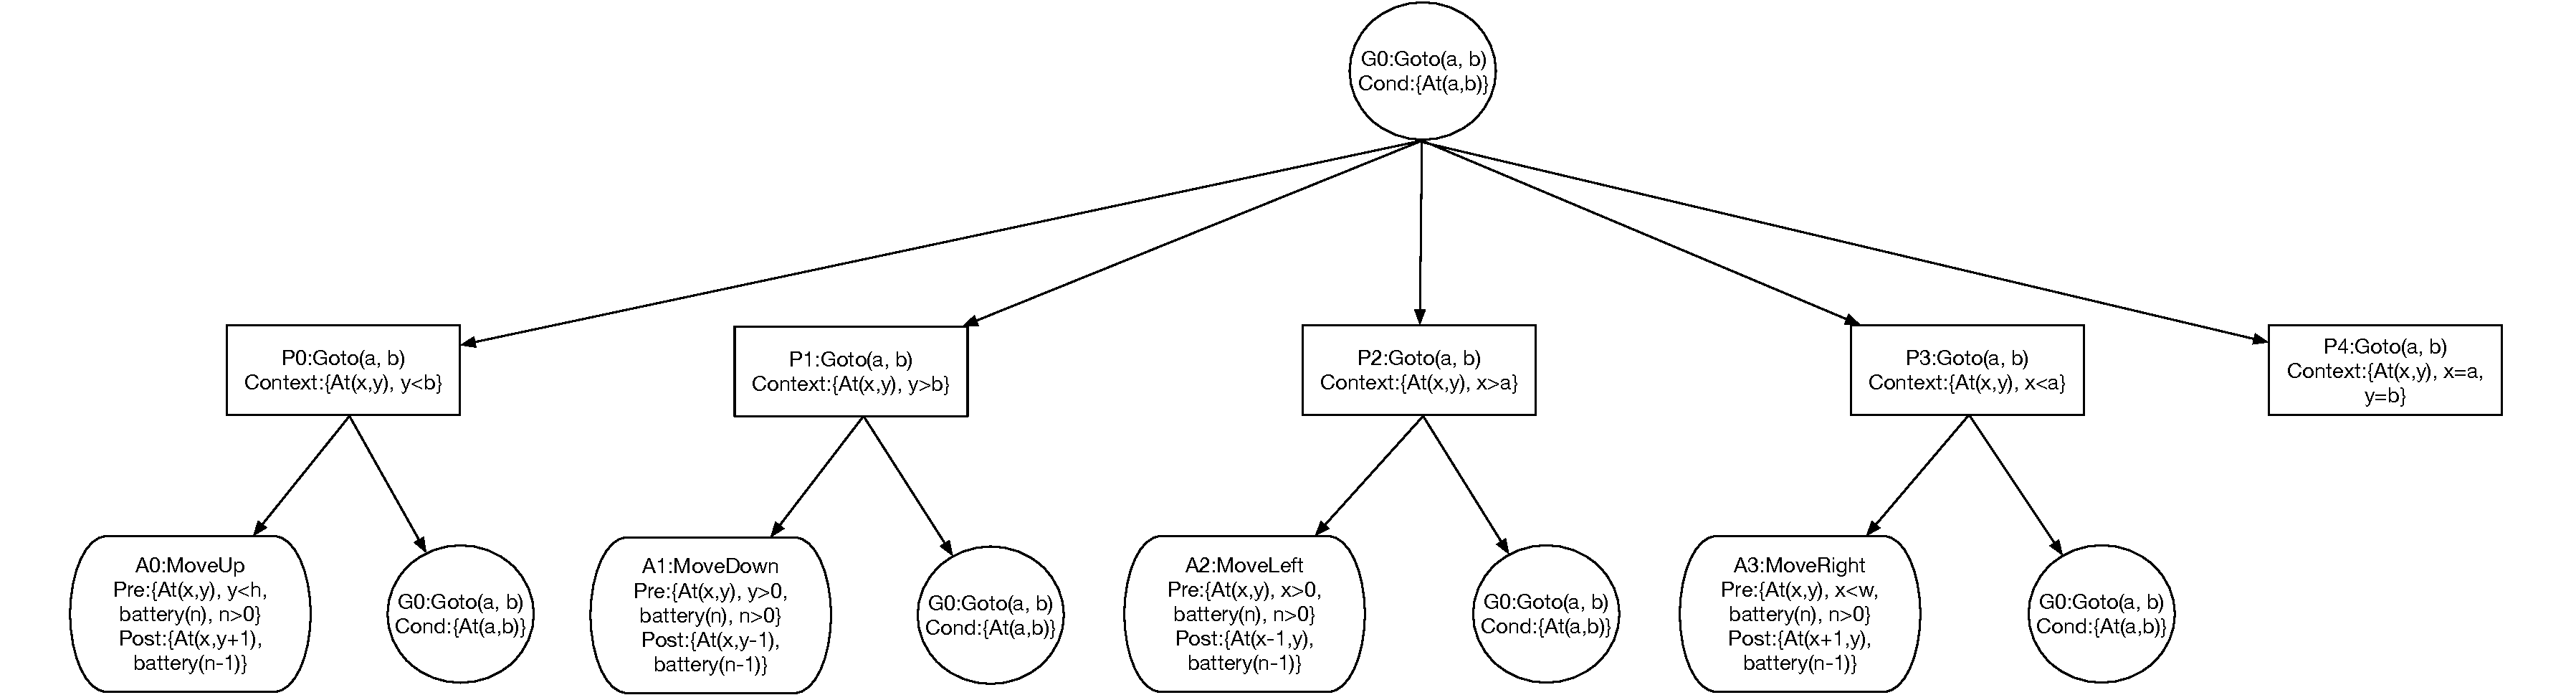
\includegraphics[width=0.9\textwidth]{./figs/MarsRover_GPT}
\caption{Example goal-plan tree.}
\label{fig:gpt}
\end{figure*}

% Benefits of GPT representation
目标计划树直观地展现了智能体目标、计划和动作之间的关系。除此以外,目标计划树还可用于记录实现目标或执行计划和动作所需的前置条件(Precondition)以及执行的结果,后置条件(Postcondition)。计划的前置条件指的是执行计划前需要满足的条件,如果前置条件不满足,则计划无法执行(动作的前置条件同理)。后置条件指的是执行动作之后的结果,对智能体所处环境造成的影响。最后,目标计划树还可以用于刻画智能体在某个环境下实现特定目标时的健壮性,Thangarajah等人基于目标计划树提出Coverage和Overlap的概念以刻画智能体程序的健壮性。其中Coverage表示一个意图当前的目标或子目标至少有一个计划可执行情况下可能的环境状态占比;而Overlap则表示一个目标有多个(大于一个)可执行计划的情况下可能的环境状态占比。

\subsection{意图进展问题}
上一小节介绍了目标计划树的概念,本章节基于目标计划树,对BDI智能体意图进展问题进行规范定义。

BDI智能体通常有多个计划用以实现某一个目标,不同的计划根据其前置条件不同适用于不同的环境场景,前置条件满足的计划被称为可应用计划(Applicable Plan)。
% plan selection
当同时有多个可应用计划是,智能体需要考虑选择哪一个计划用以实现相应目标,该问题被称为计划选择问题(Plan Selection Problem)。计划选择会影响到并发执行的其他目标,因为不同的计划有着不同的执行结果,这些执行结果可能会影响其他目标下计划或动作的前置条件。这种影响可能是负面的,例如一个计划执行之后使得其他目标下的某些计划的前置条件失效,也有可能是正面的,例如一个目标下的某些计划的前置条件在初始时是不满足的,当执行其他目标下的计划之后使得其前置条件满足。

% intention selection
另一方面,当智能体有多个意图时,下一步该执行哪个意图的问题被称为意图选择问题(Intention Selction Problem)。意图选择问题同样也会影响目标的实现,不合理的意图选择可能会造成各个意图中的前置条件相互破坏,导致无法实现任何一个目标(单个目标本身可以顺利实现),而合理的意图选择则可以使得多个意图产生协同效应,相互促进执行。

% IPP
意图进展问题(Intention Progression Problem)为上述两问题的结合,即同时考虑计划选择问题和意图选择问题。意图进展问题是本文所研究的问题的基础。为了规范并一般化地表示意图进展问题,本文基于目标计划树对意图进展问题进行定义。一个意图的进展实际对应于一个目标计划树中一条从根节点到一个叶子结点的路径。目标计划树中的任何一条从根节点至叶子节点的路径都对应于实现其顶层目标的一种方式。每一条路径都包含一系列的计划、动作和子目标,如果他们都被成功执行,即可实现顶层目标。如此,智能体的执行过程可看作多个目标计划树执行路径的相互交错,即对应于意图进展的并发执行。

%
在不同场景下对智能体性能的评估标准可能不同,例如,有时智能体完成目标的数量越多越好,而有时公平性更重要,多个目标的完成时间越接近越好。为了在社会仿真模拟场景下提供一个一般化的意图调度方法,本文假设对某一场景下的智能体有一价值函数$f_{\mu}$,$f_{\mu}$的输入参数为智能体状态信息,并返回一个评估值,代表智能体当前的性能表现。$f_{\mu}$函数可由用户自定义,以应用于不同的问题场景。

% definition
基于上述内容,意图进展问题可被理解为:如何选择多个目标计划树的交错执行路径,使得最终基于$f_{\mu}$获得最大的价值。具体的,给定一组表示智能体意图的目标计划树集合$\{t_1, \dots, t_n\}$,当前环境信息$Env$,智能体的初始状态$S_0$,需要实现的目标集合$G_0$以及当前问题中的价值函数$f_{\mu}$,智能体在每一个运行周期中求解并执行目标选择,计划选择以及意图选择,直到某个最终状态$S$停止运行,要求最终状态$S$使得有效函数$f_{\mu}$的值最大,即智能体从初始状态$s_0$开始进行目标计划树的交错执行,不存在某个最终状态$S^{\prime}$,使得$f_{\mu}(S^{\prime})$的值大于$f_{\mu}(S)$。

\chapter{智能体意图调度理论和方法}
本章主要介绍本文提出的相关方法所依赖的核心算法--蒙特卡洛树搜索算法以及其在目标计划树模型下的具体应用。
\section{蒙特卡洛方法}
蒙特卡洛方法是一类基于随机采样对决策或状态进行评估的方法。
% 重要性
该方法在多个领域都有重要应用,例如在棋类游戏中进行随机模拟采样,以此来对不同决策所带来的收益进行评估;又如在统计物理学与数学问题渗透问题中,利用现代计算机的高速计算能力进行随机采样以计算不同情况下的渗透概率。
% 特点,举例说明,model probability,额外说明episodic
蒙特卡洛方法的特点在于使用多次随机采样结果的平均值对某一状态或决策进行价值评估。其样本来源可以是智能体与实际环境的交互流程,也可以是智能体基于对环境的认知,进行的随机模拟。例如,在棋类游戏中,若需对当前棋手的胜率进行估计,则可以基于当前棋局进行多次随机模拟,每次模拟都在某一方获胜的情况下停止。最终统计各棋手在所有模拟流程中的胜利与失败次数,并基于此计算胜率。虽然蒙特卡洛方法需要环境模型,例如棋类游戏的规则,但是其并不需要精确的决策结果的概率分布,例如对手棋手的策略,而仅需要可以生成样本的模型。在众多领域,获得模型的生成样本比获得完全的概率分布更加容易。另有一点需要注意的是,蒙特卡洛方法仅应用于幕式模型(Episodic Model),即环境的运行最终会停止,而不会无限运行下去。

% 优点
蒙特卡洛方法有多个优点,
首先,它是一个领域无关(Domain Independent)的方法,也就是说它仅需知道环境的基本运行规则,而不需要环境的所有信息。
%
其次,蒙特卡洛方法可以基于多次的随机采样采样提供较为准确的价值评估,基于大数定律(Law Of Large Numbers),随机变量的期望值可以由很多个样本值的平均值近似求得,因此其准确性在理论上得到保障。
%
另外,在随机性较强、可能性众多的场景,蒙特卡洛方法由于其自身随机性的特点,在进行采样时会考虑到所有可能的情况,而不会只考虑到其中一部分。
%
最后,蒙特卡洛方法可仅针对于环境的某一个状态进行评估,而不需掌握环境所有可能状态的评估值,因此当需要对环境的某一特定状态进行价值评估,蒙特卡洛方法比其他方法(如动态规划方法)更加高效。

% 缺点
然而,蒙特卡洛方法也有一些缺点。例如基于其随机采样得到的评估值仅仅只是近似值,而不是一个准确值。在某些场景下,考虑到计算开销,蒙特卡洛方法只能进行少量的随机采样,而无法进行多次的随机采样,这种情况下即使有大数定律的支撑,由于样本量少,可能使得评估价值与实际值会有较大偏差。
%
另外,蒙特卡洛方法对多个不同环境状态的评估都是相互独立的,这意味着对某一个环境状态的评估过程以及结果并不会影响其他环境状态的评估。这种特性使得人们无法通过蒙特卡洛方法建立不同环境状态直接的联系。相较于此,树搜索则可以基于不同环境状态之间的因果关系以及动作结果的概率分布,构建树形结构,其清晰直观地展现了不同环境状态直接的关联性。树形结构明确地展现了不同动作可能导致的结果以及一连串动作导致的结果等,这在众多决策问题中可以提供有效的指导性。而蒙特卡洛方法仅仅只有基于随机采样得到的数值。
\section{蒙特卡洛树搜索(Monte-Carlo Tree Search)}
蒙特卡洛树搜索是一种针对决策问题的启发式搜索算法\cite{DBLP:conf/aiide/ChaslotBSS08,chaslot2006monte,DBLP:conf/ecml/KocsisS06},其结合了蒙特卡洛方法随机性的优点以及树搜索精确性的优点,在人工智能领域有着重要应用。2016年,研究人员将蒙特卡洛树搜索与神经网络(Neural Network)相结合,开发出了能够击败世界围棋冠军的ALphaGo\cite{DBLP:journals/nature/SilverHMGSDSAPL16},引起各界广泛关注。此外,蒙特卡洛树搜索还被应用在其他游戏中,如桥牌、克里比奇牌以及电子游戏《全面战争:罗马2》中。最初蒙特卡洛树搜索主要应用于游戏领域,但其树搜索以及随机模拟的特性使得它可被应用于其他问题领域,只需问题的求解过程可以通过树形结构表示即可。

蒙特卡洛树搜索通常在智能体当前的环境状态下运行,用于求解当前状态的最佳决策。在执行完一个决策之后,智能体进入到下一个环境状态,这时蒙特卡洛树搜索将被再次调用用于求解下次的决策,如此循环往复直到智能体到达某个最终状态。每一次蒙特卡洛树搜索的执行都是基于当前环境状态的对将来执行过程的模拟。

% core idea
蒙特卡洛树搜索的核心思想在于在有限给定的计算资源下专注于对某些收益最大或者最有潜力的模拟执行路径进行分析,以得到最优决策。基于当前的环境状态,其使用模拟执行轨迹的评估值对初始部分的执行轨迹进行评估,并基于评估值对初始执行轨迹进行拓展,被拓展的部分为收益最大或者最有潜力的决策。由此,初始部分的执行轨迹随着蒙特卡洛树搜索的执行越来越具体,并随着扩展,初始部分的执行轨迹占比也越来越大。
%rollout
在每一次的模拟执行过程中,随机模拟执行的流程占比最大。随机模拟执行的评估值最终将用于刻画某些初始决策的价值(这些决策往往是智能体在不久的将来所可能作出的决策)。在随机模拟过程中,智能体将执行随机策略(Rollout Policy),只要随机策略相对简单且环境模型并不复杂,蒙特卡洛树搜索可以在有限的计算资源下生成大量模拟执行路径。
% only part of state-action paris are considered
模拟执行的流程只与一部分初始决策有相关性,这些初始决策与其所处的环境状态共同构成了树形结构。其中每个节点记录了环境状态,该状态被经历的次数以及状态的评估值。每个边对应于智能体的一个决策。蒙特卡洛树搜索增量式地基于模拟路径的评估值对树进行扩展,被拓展的部分为价值高或者有潜力的状态。每一次的模拟执行都是从根节点(对应于智能体的当前状态)出发,进过部分子节点并最终达到某个叶子结点后离开搜索树;离开搜索树之后,根据随机策略进行多次的随机模拟得到评估值用于对经历过的树节点进行价值更新。

%
在树中进行搜索时,基于每个节点的价值进行选择性的搜索,树中的搜索策略被称为树策略(Tree Policy)。树策略可以用于平衡探索(Exploration)与开发(Exploitation),即在探索最有潜力的决策与开发最有价值的决策间进行权衡。其中最有潜力的决策为在模拟时经历次数少的决策,而最有价值的决策对应于导致最终随机模拟结果的评估值高的决策。
% UCB
在蒙特卡洛树搜索中,树策略一般使用UCB(Upper Confidence Bound,UCB)\cite{DBLP:journals/ml/AuerCF02}规则:

\begin{equation}
UCB = \overline{X}_{a} + c\sqrt{\frac{2\ln N}{N_a}}
\end{equation}

其中,$\overline{X}_{a}$为决策$a$价值的平均值,$N_a$为决策$a$被执行的次数,$N$为执行的总次数,$c$为某个大于0的常数,其作用为控制探索的程度($c$越大,该算法越倾向于探索)。

% specific
蒙特卡洛树搜索具体包括四个阶段:选择(Selection),扩展(Expansion),模拟(Simulation)以及回溯(Back-Propogation)。图\ref{fig:mcts_process}中展示了运行一次蒙特卡洛树搜索的过程。

\begin{figure*}[htb]
\centering
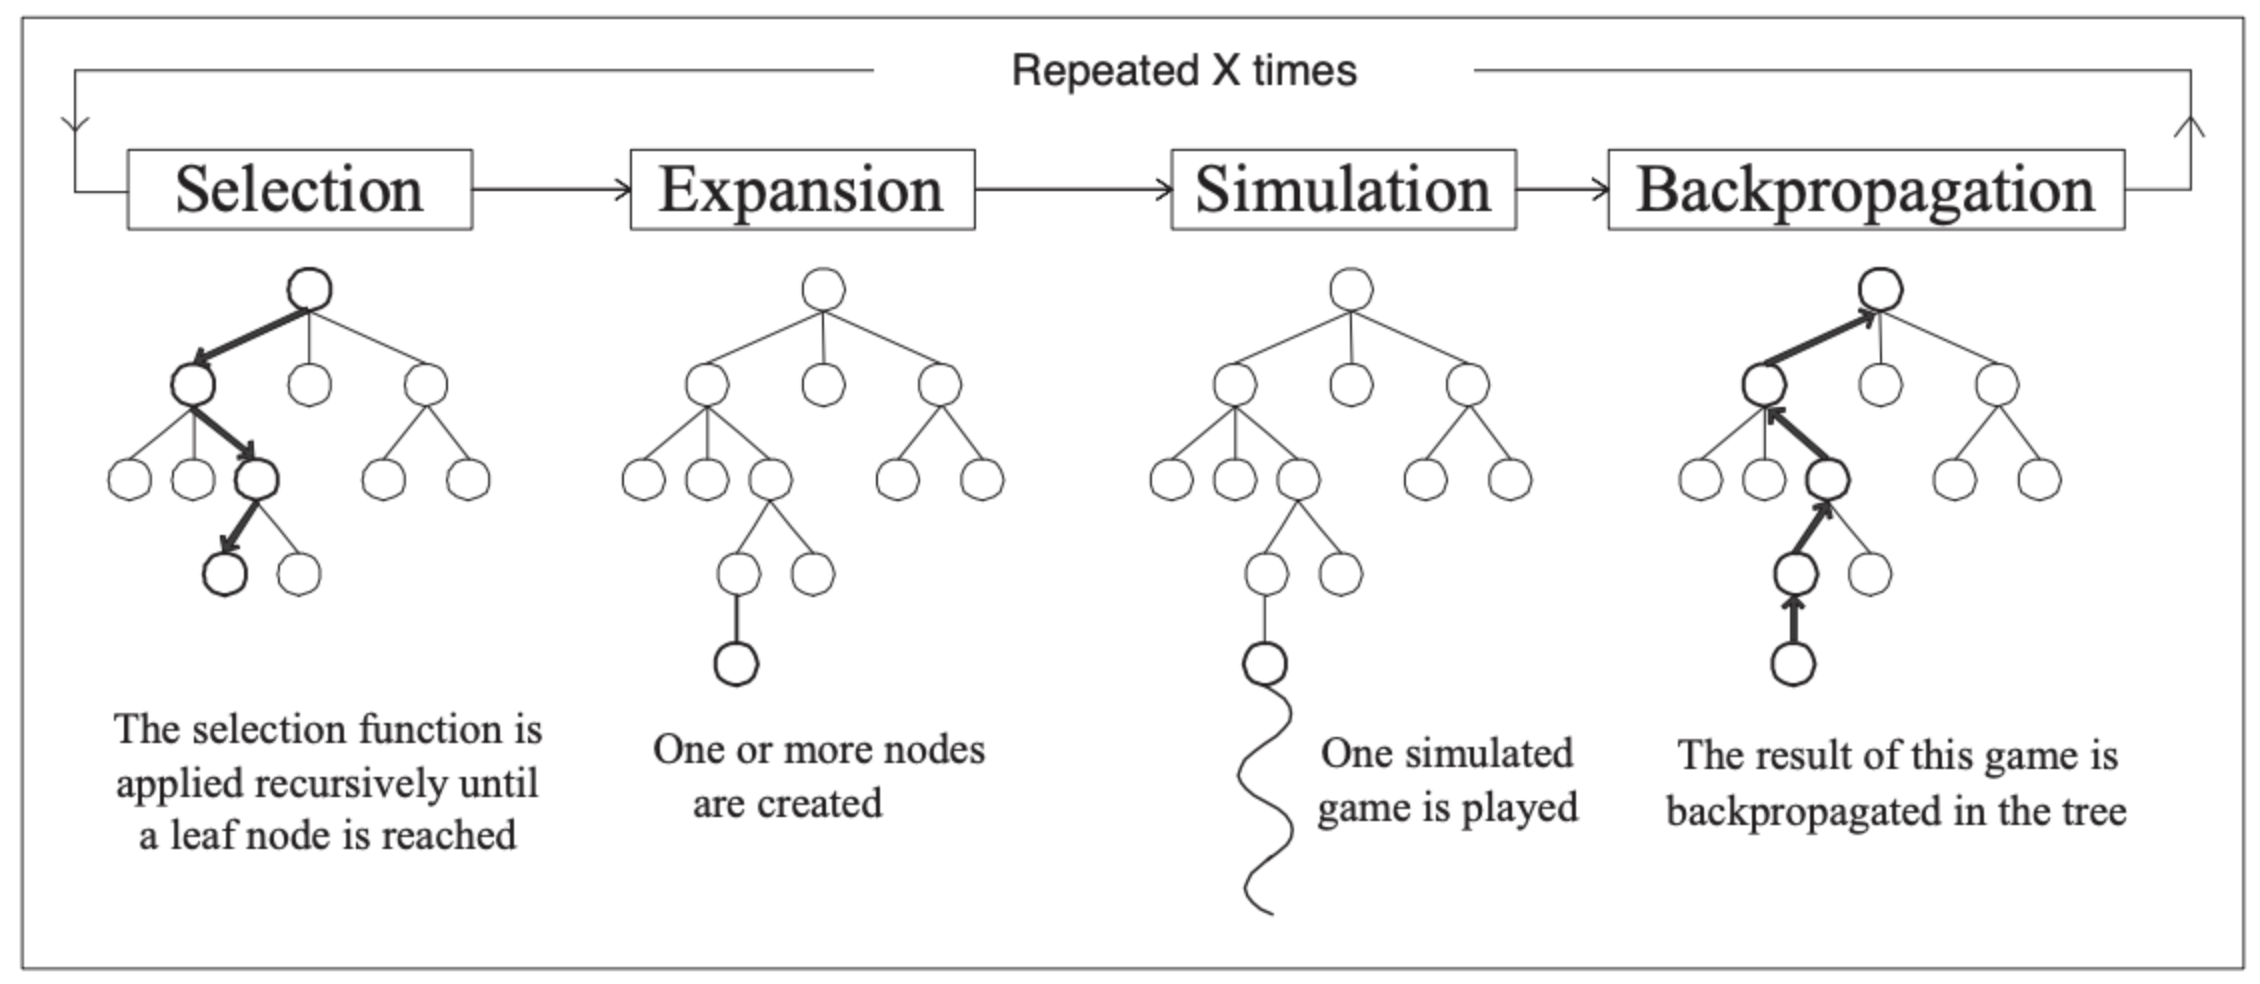
\includegraphics[width=0.9\textwidth]{./figs/mcts_process}
\bicaption{MCTS流程\cite{Sutton2005ReinforcementLA}}{Outline of MCTS\cite{Sutton2005ReinforcementLA}}
\label{fig:mcts_process}
\end{figure*}

\paragraph{选择}
在选择阶段,自根节点开始,根据树策略不断迭代选择子节点,直到到达某个叶子结点$n_e$。最终选中的叶子结点将用于接下来的扩展。
\paragraph{扩展}
在扩展阶段,基于被选中的叶子结点$n_e$,生成一个或多个新节点作为$n_e$的子节点。这些新生成的节点根据$n_e$节点中的状态所能执行的动作而生成。每一个新节点都对应于在$n_e$状态下执行一个动作的结果,而连接$n_e$与新节点的边则对应于该动作的执行。需要注意的是,若$n_e$状态下无可执行的动作,则不会有新的节点生成。新生成的节点用于下一步的模拟。
\paragraph{模拟}
在模拟阶段,首先选中某一个新生成的节点$n_s$(如果在扩展阶段没有新节点的生成,则选择当前叶子结点),从$n_s$节点中的状态开始,使用某个随机策略进行随机模拟执行,直至某个最终状态。至此可知,蒙特卡洛树搜索的一次完整的模拟执行轨迹由两部分组成:在树搜索阶段根据树策略生成的执行轨迹,以及在随机模拟阶段根据随机策略生成的执行轨迹。随机模拟过程中使用的策略可以是完全随机,以应用于多种问题场景,也可以根据具体的问题场景由用户自行控制以获得更准确的价值评估或节省计算开销。
\paragraph{回溯}
最后,在回溯阶段,上一阶段获得的最终评估值被反向传播至搜索树中所经历的每个节点以更新其相应的价值。

蒙特卡洛树搜索循环迭代地执行上述四个步骤直到用尽给定的时间或耗尽其它的计算开销。最终,根据某种策略,根节点状态下的某个动作被选中并返回给智能体作为最终的决策。最终的选择策略有多种,例如选择根节点状态下可执行的价值最高的动作,或者是选择被访问次数最多的动作等。用户可以根据具体的应用场景自行选择合适的策略。总之,该最终选择的动作即为智能体下一步真实执行的动作。
%
在执行完该选中的动作之后,环境被改变,进入下一个状态,蒙特卡洛树搜索再次被执行以确定下一个要执行的动作。新一轮的算法执行可以根据新的环境状态重新自根节点开始构建搜索树,也可以基于上一次算法执行所生成的搜索树进行构建,以节省计算开销。

% @TODO: advantages of MCTS

\section{目标计划树模型下MCTS的应用}\label{SA}
Yao等人提出基于蒙特卡洛树搜索的\SA \cite{DBLP:conf/atal/YaoL16}算法用于在目标计划树模型下对智能体的意图进行调度。本节的主要内容是对\SA 算法进行介绍(由于\SA 算法的应用场景与本文有所不同,所以略去了算法的一些无关部分)。

\SA 算法有4个输入参数:
\begin{enumerate}
  \item 智能体当前的意图集合 I(以目标计划树的形式表示),
  \item 智能体当前所处的环境状态 E,
  \item 每次算法所执行的迭代次数 $\alpha$, 
  \item 以及每次迭代迭代中随机模拟的执行次数 $\beta$,
\end{enumerate}
其中$\alpha$和$\beta$参数决定了算法运行的计算开销,可由用户自定义。\SA 最终返回某个意图中的下一步选择以供智能体在当前周期执行。\SA 算法的具体流程如算法\ref{alg:SA}所示:

\begin{algorithm}
\caption{返回当前周期执行的动作}\label{alg:SA}
  \begin{algorithmic}[1]
    % \PROCEDURE{$SA(I, E,\alpha,\beta)$}{}
    \STATE input:$(I, E,\alpha,\beta)$
    \STATE $n_0 \gets node_0(I,E)$ \label{root}
    \FOR{$i \gets 1,\alpha$} \label{iteration begin}
      \STATE $n_e \gets MAX-UCT-LEAF-NODE(n_0)$ \label{selection}
      \STATE $EXPAND(n_e)$ \label{expansion}
      \STATE $n_s \gets RANDOM-CHILD(children(n_e))$ \label{simulation begin}
      \STATE $S \gets \emptyset$
      \FOR{$j \gets 1, \beta$}
        \STATE $S \gets S \cup SIMULATE(n_s)$
      \ENDFOR \label{simulation end}
      % @TODO: max or average?
      \STATE $V_{best} \gets maxValue(S)$
      \STATE $BACKUP(n_s, V_{best})$ \label{back}
      \ENDFOR \label{iteration end}
      \STATE \RETURN $BEST-NEXT-STEP(n_0, f_b)$
    % \ENDPROCEDURE
  \end{algorithmic}
\end{algorithm}

其中$I=\{(t_1,s_1), \dots, (t_n, s_n)\}$,$t_i$表示第$i$个目标计划树(即第$i$个意图),$s_i$表示底$i$个目标计划树的当前步骤。算法流程从代表智能体当前所处状态与意图的根节点(第\ref{root}行)开始,迭代地进行模拟执行并扩展搜索树。算法的主体循环部分(第\ref{iteration begin}-\ref{iteration end}行)对应于蒙特卡洛树搜索的四个阶段:选择、扩展、模拟以及回溯。
% selection
第\ref{selection}行对应了选择阶段:从根节点$n_0$开始,根据基于UCB的树策略不断进行选择,直到某个叶子结点$n_e$。
% expansion
第\ref{expansion}行对应了扩展阶段:基于智能体在$n_e$状态下可以进展的意图,生成新的树节点。在这一阶段,依次对智能体的每个目标计划树进行检查,若目标计划树当前的步骤为动作节点,那么直接生成一个新的搜索树节点,对应于执行该动作的结果;若当前步骤为(子)目标,那么检查是否有可用的计划,若有可用计划则递归地对每个可用计划的第一个步骤进行检查:若为动作节点则直接生成相应的新搜索树节点,否则继续检查。由此得知,每一个新节点就是一条意图的部分执行路径,且该路径的最后一个执行步骤为动作。最后,随机选中一个生成的节点$n_s$作为接下来模拟阶段的开始状态。
% simulation
第\ref{simulation begin}-\ref{simulation end}行对应了模拟阶段:在该阶段,基于完全随机的策略(或者用户指定策略)进行目标计划树的进展,直到无法执行下去或所有目标都被实现,即所有当前步骤的前置条件都不满足(对于目标则是无可用计划),或所有顶层目标指定的状态都被实现。
% backup
在$\beta$次的模拟流程结束之后,选择$\beta$次模拟中最大的评估值进行反向传播。该价值反向传播至从$n_s$到根节点$n_0$路径上的所有节点。除了智能体的意图以及环境状态信息,每个节点还记录了其他统计信息:节点被访问次数,回溯价值总和以及最佳的回溯价值。

在$\alpha$次的循环执行之后,\SA 算法最终基于某个评价标准$f_b$返回当前周期(对应于树搜索的根节点$n_0$)最佳的意图进展策略(第\ref{back}行)。$BEST-NEXT-STEP$方法根据$f_b$对根节点的孩子节点进行比较,并返回到达某个最优节点$n_p$的边(即下一步的选择和执行的动作)。$f_b$可以由用户自定义,如以节点的访问次数为标准或以节点的最高价值为标准等。最终智能体将实际执行该选择的步骤,并在执行之后根据环境反馈更新自身信念和意图。

\subsection{\SA 算法与BDI智能体的实践推理过程}
第\ref{background}章中提到BDI智能体的实践推理过程包括慎思与手段推理,分别对应于意图选择和计划选择。然而,在\SA 算法中,慎思与手段推理实际上被合并为一步。另外,\SA 算法针对的问题是如何去实现给定的一组目标,而对于要实现哪些目标则在\SA 算法的考虑范围之外,通常由用户给定。当智能体接收到一个新目标之后,\SA 算法不仅要确定接下来要实现哪个目标,还要确定使用哪一个计划来实现该目标;在该过程中还要考虑到多个意图之间的相互交错带来的影响,避免负面的影响并利用多意图间的协同效应,最终得到收益最大的意图进展路径。

%
在众多智能体编程语言中,意图选择和计划选择策略往往是默认的先来先服务(First In First Out,FIFO)或轮询(Round Robin,RR)算法,或需要用户自定义,例如在Jason\cite{bordini2007programming}中,计划选择时默认选择可用的第一个计划,而意图选择算法为轮询。
%
另外Jason也提供用户自定义的策略编程接口$S_O$和$S_I$分别对应于计划选择策略和意图选择策略。
% compare to jason
虽然提供自定义决策编程接口可以使得智能体更加灵活,但是自定义策略需要有一定程度的某个问题领域的专业知识。若要将其应用多种场景,则需要进行多次的策略定制。另外,决策策略一般为智能体编程语言层面的设计,使用不同智能体编程语言对决策策略的自定义方式可能不尽相同,这一定程度上增加了程序员的负担。对比之下,\SA 算法则可以让用户专注于需要解决的问题本身,即如何定义价值函数,而无需考虑编程语言的底层实现。

%
在目标计划树中,每个节点都有其相关的条件:目标有其目标条件,计划有其前置条件,动作有其执行结果。虽然这些条件由用户自行设定,需要一定的额外工作,但是于\SA 算法可以有效利用这些条件来避免意图间的冲突以及利用意图间的协同效应以高效地执行智能体程序。

\chapter{支持维持型目标的意图调度算法}\label{mg}
本章将提出一种基于\SA 的意图调度算法\SAM ,\SAM 支持同时对实现型和维持型目标的调度。其中维持型目标考虑到了在第\ref{background}中提到的被动维持型目标和主动维持型目标。另外,本章对\SAM 的性能在动态和静态环境下进行了实验分析,并与Duff等人提出的PMG\cite{DBLP:conf/atal/DuffHT06}算法进行了比较,实验结果表明\SAM 的性能表现相对PMG有显著优势。
\section{维持型目标}
目前大多数对BDI智能体意图调度方面的研究主要考虑的是实现型目标,即指定某一个智能体要去达到的环境状态,一旦智能体通过执行动作达到了该指定状态,实现型目标即被抛弃。
% MG
但是在许多问题场景中,智能体还必须持续地保持某个环境状态一段时间,例如一个火星探测器必须确保它总是有足够的电池电量用以返回基地充电,否则它可能会因耗尽电池而搁浅。为了避免这种情况,一个理性的智能体需要有一个针对电池的目标,在其电量变得很低之前返回基地充电。这种目标被称为维持型目标,其指定了一个智能体需要持续维持的环境状态。

% Execution

当智能体接收到一个实现型目标时,他将执行一个计划来实现该实现型目标,并在条件实现放弃该目标。
%
然而,对于维持型目标,在其指定的维持条件为假之前,接收该目标不会导致任何动作的执行。而一旦维持条件不满足,智能体就会执行一个计划以修复该维持条件,该行为对应于被动维持型目标;或者当智能体认为该维持条件在不久的将来会不满足时,便会执行一个计划以防止维持条件在环境中失效,该行为则对应于主动维持型目标。只有当智能体不再需要维持条件时,维持型目标才会被抛弃。
% PMG
目前已有一些针对维持型目标的研究方法被提出,Duff\cite{DBLP:conf/atal/DuffHT06}提出了一种基于SI的意图调度方法PMG,该方法可用于决定是否接收一个新的实现型或维持型目标,以及在维持条件满足的情况下,何时采取预防性的措施以防止该维持条件失效。
% more specific
具体地,每次接收到一个新的目标时,智能体都会判断其是否与当前的维持型目标有冲突。如果这个新目标会与一个或多个现有的维持型目标发生冲突,智能体首先会采取预防措施以确保维持型目标在将来不会被破坏,在这之后才去执行该新目标。
% their problem
然而,PMG算法并没有考虑到智能体多个意图间的相互影响。
% maybe include the work of Hindriks?

\section{目标的表示与问题定义}
% AG and MG representation
以下为维持型目标的规范表示:
\paragraph{维持型目标}
维持型目标定义了某个智能体需要维持的环境状态\cite{DBLP:journals/ci/DuffTH14},一个维持型目标以一个四元组表示:
$$<G_m,C_m,Pls,t>$$
其中$G_m$为该维持型目标的名称,$C_m$为维持条件,$Pls$为一组用于修复该维持条件的计划,$t$为该维持型目标的持续时间(时间结束后该目标就被抛弃)。

和简单的实现型目标不同,根据维持条件$C_m$的破坏能否被可靠地预测,维持型目标可以以不同的方式实现。具体的实现方式有两种:被动维持型目标与主动维持型目标。在被动维持型目标的实现方式中,智能体直到维持条件被破坏时才执行修复计划;而在主动维持型目标的实现方式中,智能体根据当前的认知判断维持条件是否在将来会被破坏,如果判断会真,则会提前执行修复计划以防止维持条件被破坏。上述两种实现方式的具体定义如下:
\paragraph{被动维持型目标}
如果维持条件$C_m$何时会被破坏无法被可靠地预测,智能体可以被动地执行$Pls$中的某个计划,即在$C_m$被破坏之后执行。在这种情况下,维持条件$C_m$的设定较为保守。例如,如果智能体无法准确地预测智能体执行某个意图的电量消耗,则可以将$C_m$设定为一个非零的最小阈值,如20\%。该设定可以确保智能体在维持条件被破坏后有足够的电量返回基地充电。
\paragraph{主动维持型目标}
如另一方面,果维持条件$C_m$何时会被破坏能够被可靠地预测,智能体可以主动地在其被破坏之前执行某个$Pls$中的计划以防止破坏的发生。该设定可能会影响到维持条件$C_m$。例如,如果智能体可以准确地预测智能体执行某个意图的电量消耗,则可以将$C_m$设定为维持电量在零以上。

实际上,主动维持型目标和被动维持型目标是维持型目标应用的两种极端。通常来说,预测机制的可靠程度、效率和破坏维持条件的后果共同决定了该使用哪一种应用方式。

\subsection{问题的规范定义}
本章对IPP的原始定义进行拓展,加入对维持型目标的考虑,使智能体必须同时考虑对实现型目标和维持型目标的调度。另外,智能体的性能评估基于两个标准:实现目标的数量和资源消耗量。

具体地,基于目标计划树模型,同时考虑实现型目标和维持型目标下的意图进展问题可被定义为:给定一组表示智能体意图的目标计划树$\{t_1, \dots, t_n\}$以及一组表示智能体当前环境状态的条件变量$Env$,在每一个执行周期中返回一个目标计划树$t_i$中的下一个执行步骤使得智能体实现的目标数量最多且消耗的资源最少。

\section{$SA_M$意图调度算法}
本章介绍同时考虑实现型与维持型目标的意图调度算法\SAM 。\SAM 在第\SA (已在第\ref{SA}章节中介绍)的基础上进行拓展,加入对被动与主动维持型目标的考虑。
具体地,\SAM 算法修改了\SA 算法中的扩展与模拟阶段,加入了决定何时以及如何执行修复维持条件的计划的机制,以下是对SA算法的具体修改细节:
\paragraph{对扩展阶段的修改}
% Reactive
在\SAM 中,被动维持目标和主动维持目标有不同的应对机制。对于被动维持型目标,\SAM 首先检查被选中的某个拓展节点$n_s$中是否有维持条件被破坏。对于每一个维持条件被破坏的目标,生成一组新的节点,并作为$n_s$的孩子节点。这组节点对应于对应修复计划的执行。即,在$n_s$状态下,智能体可以选择像以往一样继续实现其他目标,也可以选择执行修复计划以重新恢复维持条件。对于被动维持型目标当维持条件没有被破坏时,相关修复计划的执行是被禁止的。
% Proactive
对于主动维持型目标,\SAM 假定所有维持型目标都处于激活状态,即智能体可以在任何时候都执行维持型目标的相关修复计划,只要当前该相关计划没有在执行状态即可(防止同一个计划的重复执行)。
% Special case for proactive
而当智能体没有任何实现型目标时,若没有维持条件被破坏,则不会有新的节点生成。即当智能体没有任何目标需要实现时,智能体就会处于等待状态以维持当前的状态。

\paragraph{对模拟阶段的修改}
在模拟阶段,\SAM 和SA一样,随机选择实现目标过程中可执行的动作执行。当某个被动维持型目标$G_m$被触发时,智能体除了可以选择执行实现型目标,还可以选择执行$G_m$相关的修复计划。而对于主动维持型目标,\SAM 可以在没有维持型目标相关意图执行时执行其修复计划(避免同一个意图的重复执行)。修复计划同样可以与其他意图交错执行,以避免意图间的冲突以及利用意图间的协同效应。

当以下三个条件中的任意一个满足时,模拟阶段即停止:
\begin{enumerate}
  \item 所有的实现型目标都已完成并且没有维持目标被触发。
  \item 当前状态下无法实现剩余的实现型目标。
  \item 所有维持型目标的维持条件在当前状态下都无法修复。
\end{enumerate}

\section{实验}
本章在多种场景以及不同难度下对 \SAM 的性能进行评估,并与现有的的支持维持型目标的调度算法PMG\cite{DBLP:conf/atal/DuffHT06}进行比较。

\subsection{实验场景介绍}
以下实验基于一个火星探测器的模拟场景(Mars Rover Simulator)对\SAM 算法的性能进行评估。该模拟环境为一个网格,由20 $\times$ 20个小方格组成(见图\ref{fig:marsrover})。
\begin{figure}[h!]
\centering
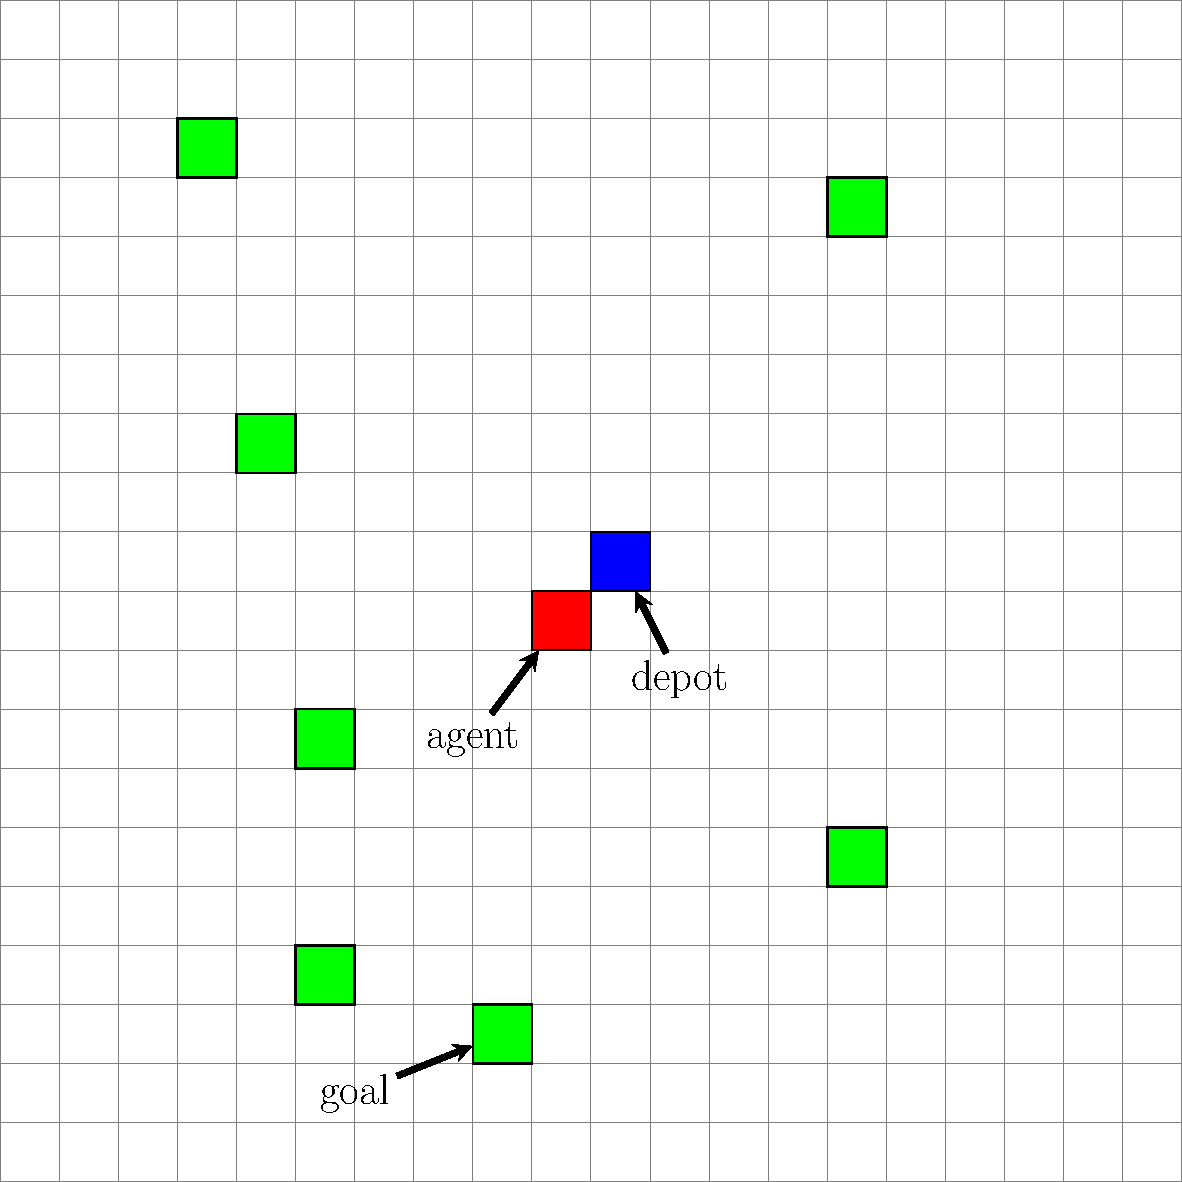
\includegraphics[scale=0.4]{./figs/mg_example}
\captionsetup{justification=centering}
\bicaption{火星探测器例子}{A Mars rover example}
\label{fig:marsrover}
\end{figure}

% introduction to the Mars rover example
网格中每个方格都是一个智能体可以到达的位置,由(x, y)所表示,其中x和y分别为x坐标与y坐标的值。
%
本实验中假设最左下角的方格坐标为(0, 0),最右上角的方格坐标为(19, 19)。
% 
火星探测器智能体被放置于某个方格中,并按要求以访问网格中某些位置为目标执行相关计划。该智能体一共可以执行4个动作以进行位置的移动:向上移动一个单位,向下移动一个单位,向左移动一个单位以及向右移动一个单位。
% 
另外,每一次的移动都会消耗1点的电量,当电量较低时,智能体可返回基地(10, 10)进行充电(假设基地有无限的电量供应)。
%
该场景下相应的目标计划树可见图\ref{fig:gpt}。
\subsection{实验设定}
本文假设在以下所有实验中,智能体每次都从基地出发,其访问的目标地点都是随机生成的\footnote{注意,同一个地点不会生成多个目标。}。
% measuring the agent
本实验根据两个指标对智能体性能进行评估:实现目标的数量以及消耗的电池电量。具体地,首先将基于实现目标的数量对智能体进行评估,实现数量越多,性能越好;如果不同的智能体实现目标的数量相同,则将基于电量消耗进行性能评估,消耗电量越低,性能越好。

本文将\SAM 与Duff等人提出的方法\cite{DBLP:conf/atal/DuffHT06}进行比较,实验考虑到了包含\SAM 等一共6种方法:

\begin{itemize}
\item \textbf{No maintenance goal (NMG)}: 该方法假设智能体的移动不会消耗电量,因此智能体无需返回基地充电。该方法以FIFO的规则实现目标,在duff 等人的文章\cite{DBLP:conf/atal/DuffHT06}中有所描述。
\item \textbf{Reactive maintenance goal (RMG)}: 该方法假设智能体无法可靠地预测维持条件何时会被破坏。因此维持型目标的实现方式是被动的,以此确保智能体有足够的电量返回基地充电。当维持型目标被触发时,智能体首先将返回基地充电,然后再尝试实现其他目标。该方法与\cite{DBLP:conf/atal/DuffHT06}中提到的RMG方法相同。
\item \textbf{Proactive maintenance goal (PMG)}: 该方法假设智能体可以基于SI方法对维持条件的破坏进行可靠的预测。因此,维持型目标的实现方式为主动型。本实验使用在\cite{DBLP:conf/atal/DuffHT06}提到的相同方法对维持型目标进行调度。
  %
即在执行其他目标之前,智能体将预测实现该目标的电量消耗情况,如果智能体在实现新目标之后没有足够的电量返回基地,那么将收件执行修复计划以保持充足的电量。

\item \textbf{No maintenance goal MCTS (NMCTS)}: 和NMG类似,该方法假设智能体的移动不会消耗电量。不同的是,实现目标使用的是SA进行调度。
\item \textbf{Reactive maintenance goal MCTS (RMCTS)}: 在该方法设定下,智能体使用\SAM 进行意图调度,维持型目标的应用方式为被动型。
\item \textbf{Proactive maintenance goal MCTS (PMCTS)}: 和RMCTS类似,该方法使用\SAM 进行意图调度,不同的是维持型目标的应用方式为被动型。
\end{itemize}

%
为了确保智能体总是有足够的电量用以返回基地,被动维持型目标的维持条件设定为$batteryLevel > 20$。这使得即使在(0,0)位置,智能体也总是有足够的电量返回基地(10,10)。
%
对于主动维持型目标,其维持条件设定为$batteryLevel > Distance(agent, depot)$,其中$Distance(agent, depot)$为智能体从当前位置移动到基地所需要消耗的最小电量。
%
一旦维持型目标被触发,其相应的修复计划就会被执行,用以返回基地充电保持或修复维持条件。
%
在以下实验中,\SAM 和\SA 的设定为执行100次迭代($\alpha = 100$),每次迭代执行10次的模拟($\beta = 10$)。另外,价值函数设定为$\#goals + \frac{1}{1 + {battery}}$,其中 $\#goals$ 为实现目标的数量, $battery$ 为用以实现目标的消耗电量。

以下实验考虑了动态与静态环境。以下的实验结果中展示的是每种方法运行100次运行次的平均性能。另外,实际上所有方法都可以在实验中实现所有顶层目标。因此,为了便于分析,本实验只使用电池消耗量来衡量不同方法的性能。
\subsection{静态环境实验}
接下来的三个实验考虑火星探测器智能体在静态环境下的表现。在静态环境下,智能体的所有实现型目标都在初始运行时给定。
\paragraph{实验一}
在第一个实验中,智能体的电池容量被设定为40,智能体需要实现目标的数量从1逐步增加至15。具体实验结果如图\ref{fig:static1}所示。
\begin{figure}[!h]
\centering
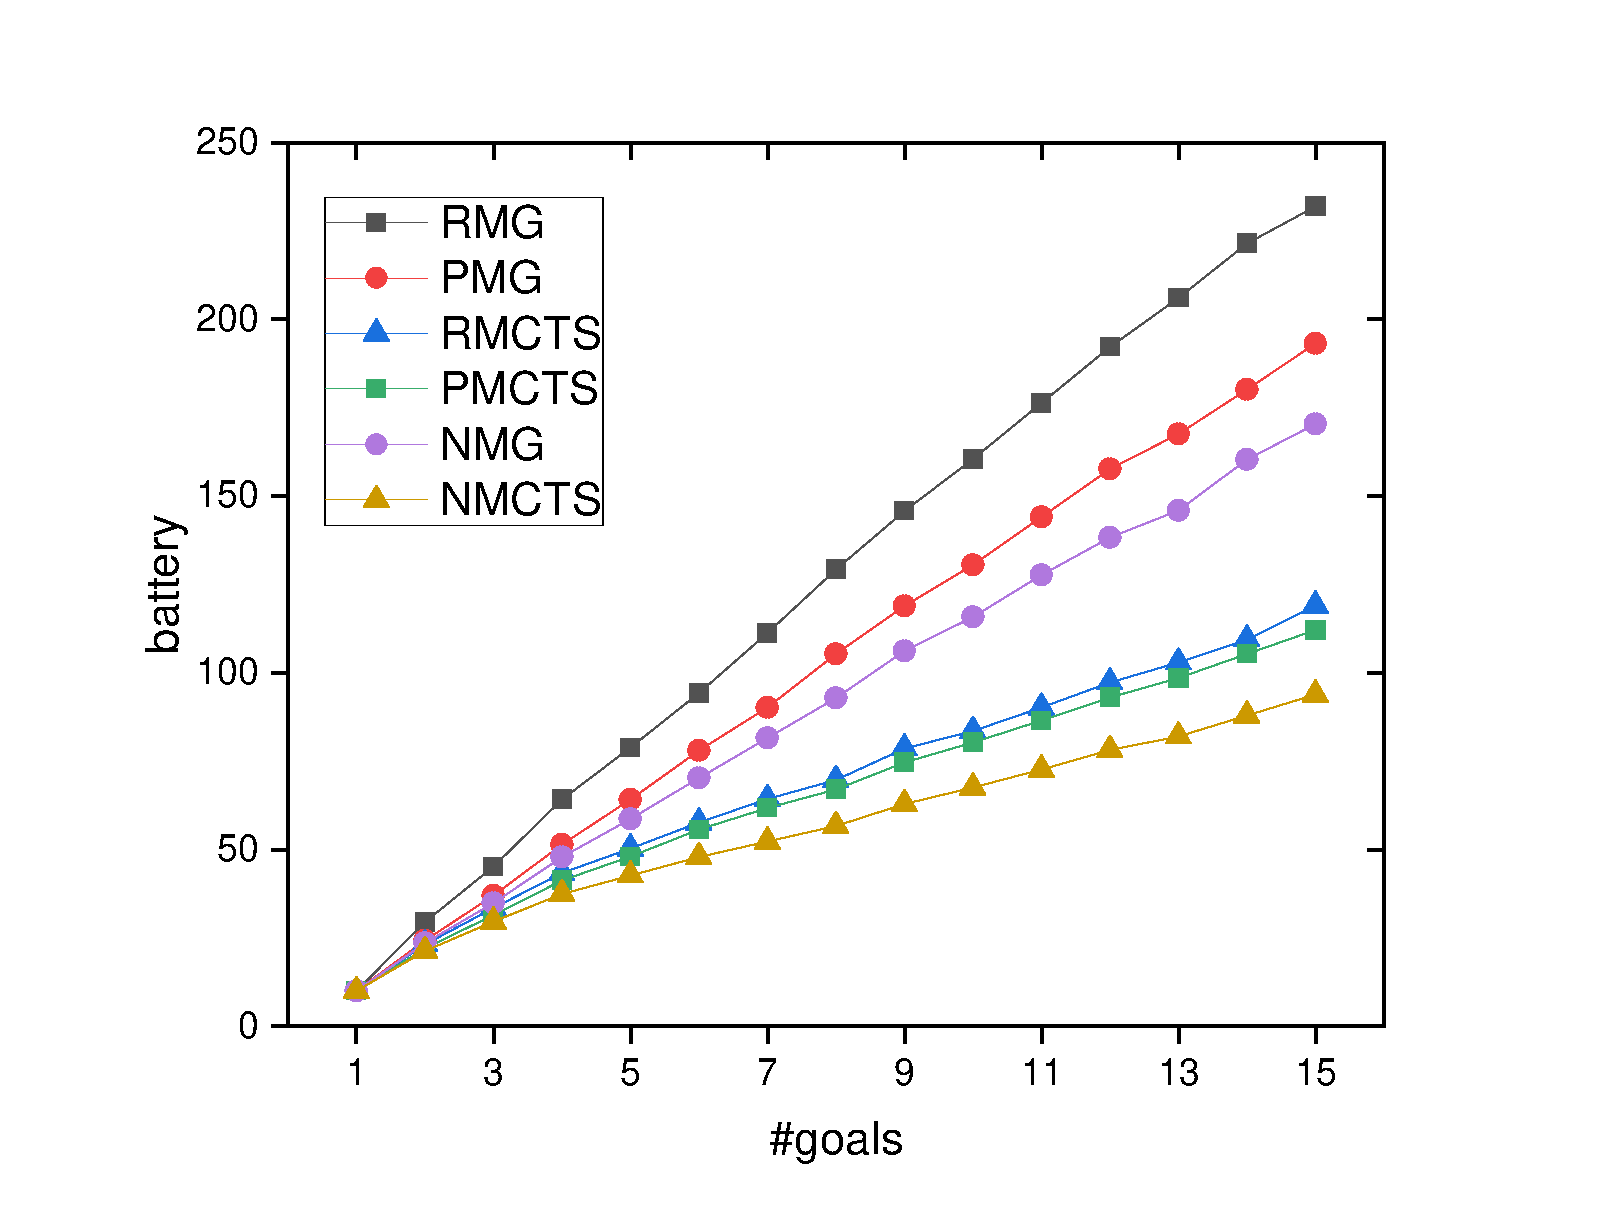
\includegraphics[scale=0.4]{./figs/gX_cY_fixCap40.pdf}
\captionsetup{justification=centering}
\bicaption{电池容量为40下的电量消耗}{Battery consumptions with fixed capacity of 40}
\label{fig:static1}
\end{figure}

从图中得知,当实现目标数量增加时,所有方法的电量消耗都有所增加。
% two baseline
由于NMCTS和NMG没有电量消耗的考虑,他们可以作为两个基准用以评估其他实际应用方法的性能。
% general
通过分析得知,基于MCTS的方法(NMCTS,PMCTS和RMCTS)性能优于其他方法。另外,使用主动维持型目标的方法的性能表现要优于使用被动维持型目标的方法。
% NMG
在所有测试情况下,RMG的性能表现最差(消耗最多的电量)。
% reason
这是因为NMG仅考虑被动地处理维持型目标,这会导致在点来电量不充足时去实现较远处的目标,导致大量无效的往返移动,浪费电量。
% PMG
相比较之下,PMG表现更好,因为其可以在实现一个目标之前对电量消耗进行评估。如果智能体经过分析后得知其会在实现目标途中触发维持型目标,那么它将首先返回基地充电,再去实现该目标。
% mcts
最后,与PMG和NMG对比,PMG和RMG有着显著的性能优势。特别是当实现目标数量变多时,他们之间的差距也越来越明显。这其中的原因在于基于MCTS的方法不仅仅能够预测维持型目标何时被触发,还能够高效地利用不同意图间的协同效应(智能体可以合并不同意图下的同一个动作以节省电量)。


\paragraph{实验二}
在第二个实验中,智能体的电量被设定为60,其他设定与实验一相同。具体实验结果如图\ref{fig:static2}所示。
\begin{figure}[h!]
\centering
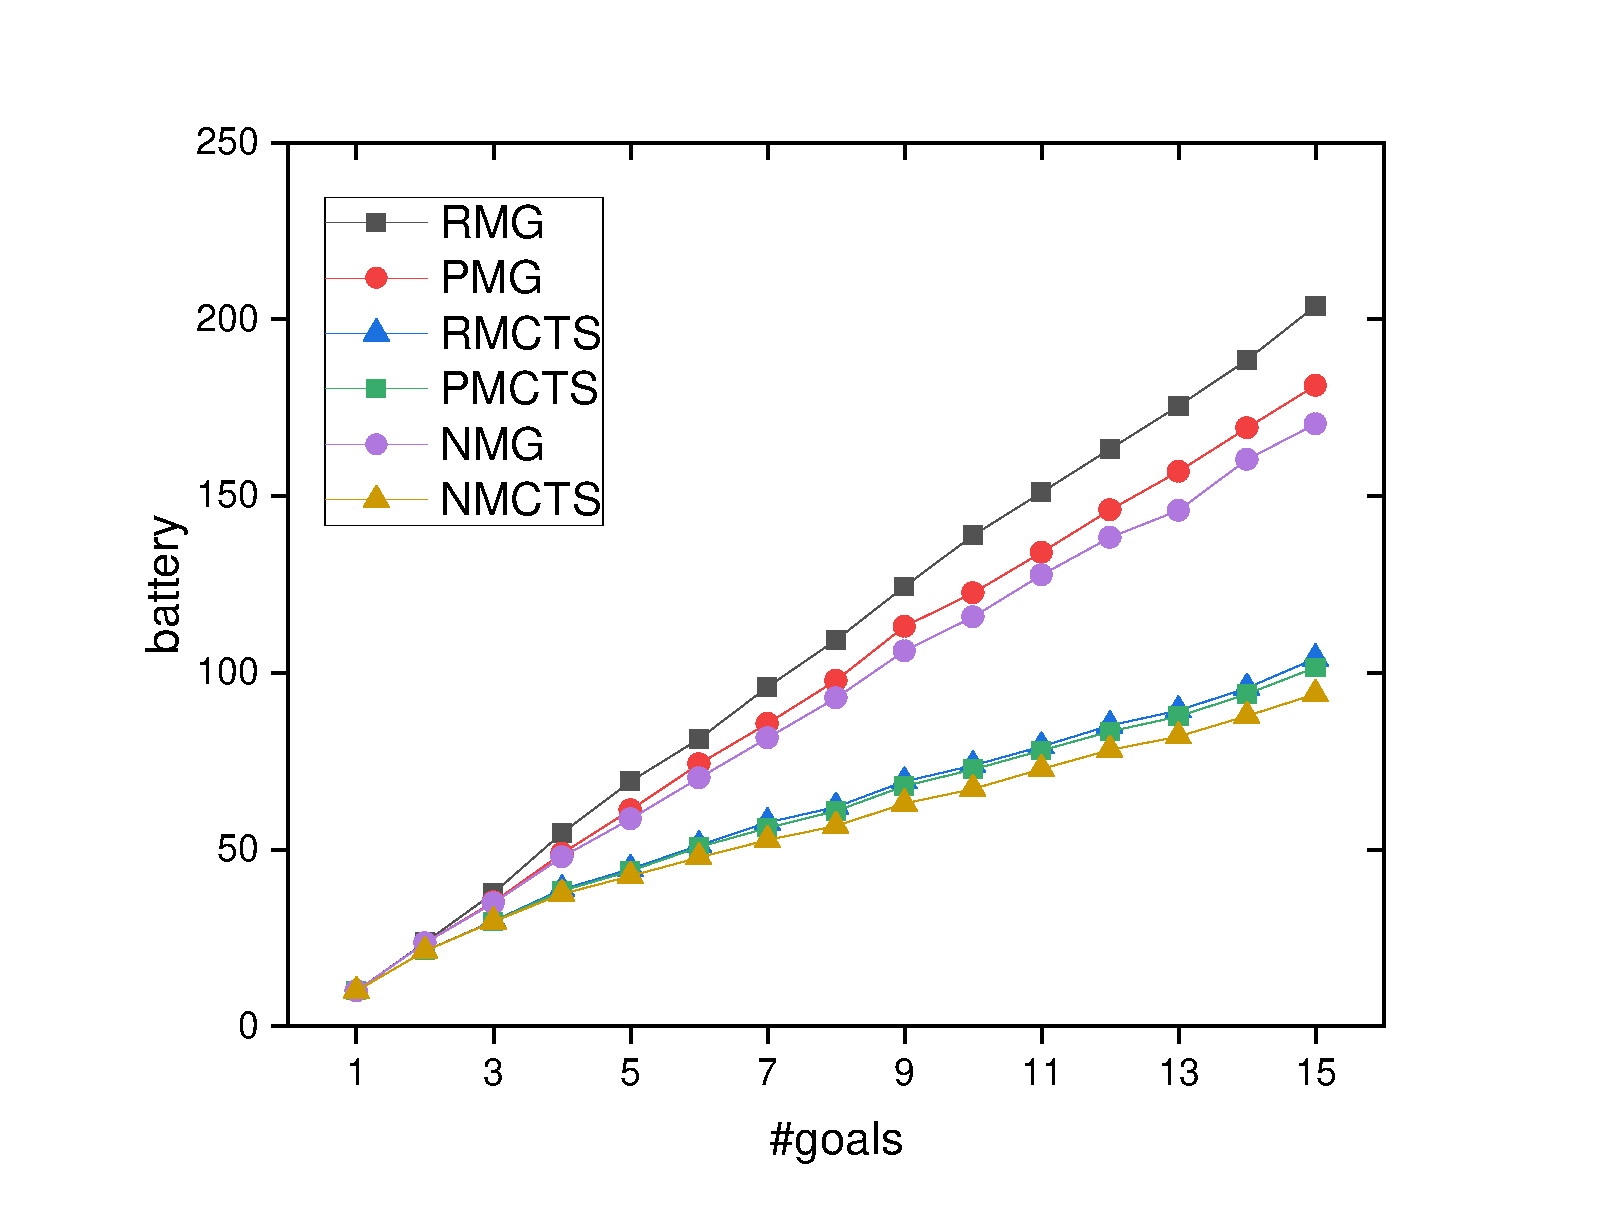
\includegraphics[scale=0.4]{./figs/gX_cY_fixCap60.pdf}
\captionsetup{justification=centering}
\bicaption{电池容量为60下的电量消耗}{Battery consumptions with fixed capacity of 60}
\label{fig:static2}
\end{figure}

从图中得知,当电池容量提升时,所有方法的电量消耗都有所降低。
%
和实验一相似,基于MCTS的方法的性能优于其他方法。在该实验设定下,基于MCTS的方法与非MCTS方法的差距更加显著。这同样也是因为基于MCTS的方法可以更高效地利用不同意图间的协同效应。
%
在实验二中,主动维持型目标的性能同样优于被动维持型目标,但是他们之间的性能差异有所减小。例如,当实现目标的数量为15时,PMCTS的电量消耗仅仅比RMCTS低2.65。
%
这是因为当电池容量变大时,维持型目标被触发的次数减小,使得被动与主动维持型目标直接的差异更小。

\paragraph{实验三}
在第三个实验中,智能体被给定固定10个目标,而电池容量从40改变至200。具体实验结果如图\ref{fig:static4}所示。
\begin{figure}[h!]
\centering
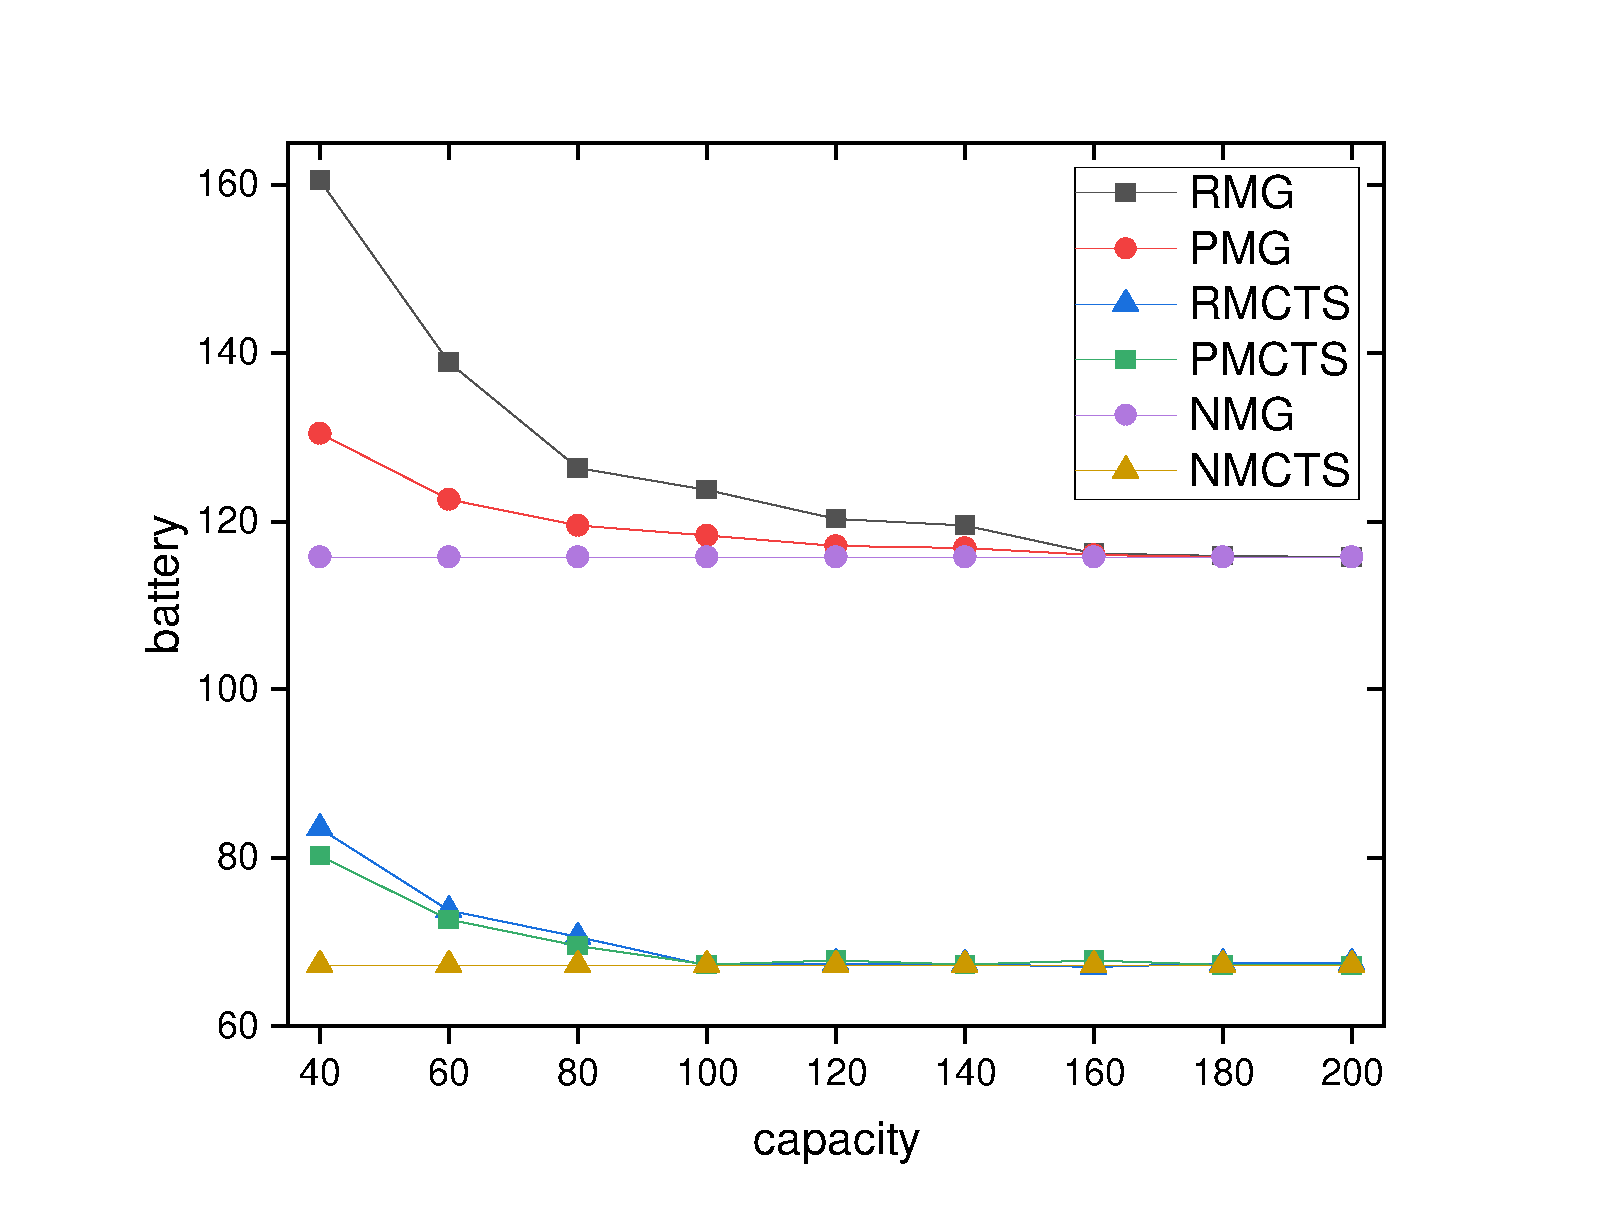
\includegraphics[scale=0.4]{./figs/cX_cY_fixG10}
\captionsetup{justification=centering}
\bicaption{目标数量为10下的电量消耗}{Battery consumptions with fixed 10 goals}
\label{fig:static4}
\end{figure}

正如图中所示,当电池容量相对较低时,增加电池容量能够显著地提升所有方法的性能。
%
而当电池容量足够大时,持续地增加电池容量并不会对智能体的性能造成明显的影响。被动维持型目标和主动维持型目标在大容量电池下有非常相近的性能表现。
%
这是因为增加的电池容量会逐渐超出智能体用以实现目标的电量所需,甚至在超过一定阈值之后,提升电池容量不会对智能体性能有任何影响。然而,基于MCTS的方法在所有测试情况下都优于其他非MCTS方法。

\subsection{动态环境实验}
为了探究不同方法在动态环境下的性能表现,以下实验假定并非所有目标都在初始时给定。相反,一些目标会在运行时分配给智能体。
%
本实验使用变量$n$来代表两个目标的分配时间间隔。即每隔$n$周期给智能体分配一个新的目标(假定执行一个动作对应一个周期)。

\paragraph{实验四}
和实验一类似,在该实验中智能体的电池容量被设定为40,实现目标的数量从1变化至15。另外,$n$的值被设定为5,即每隔5个周期给智能体分配一个新的目标。
\begin{figure}[h!]
\centering
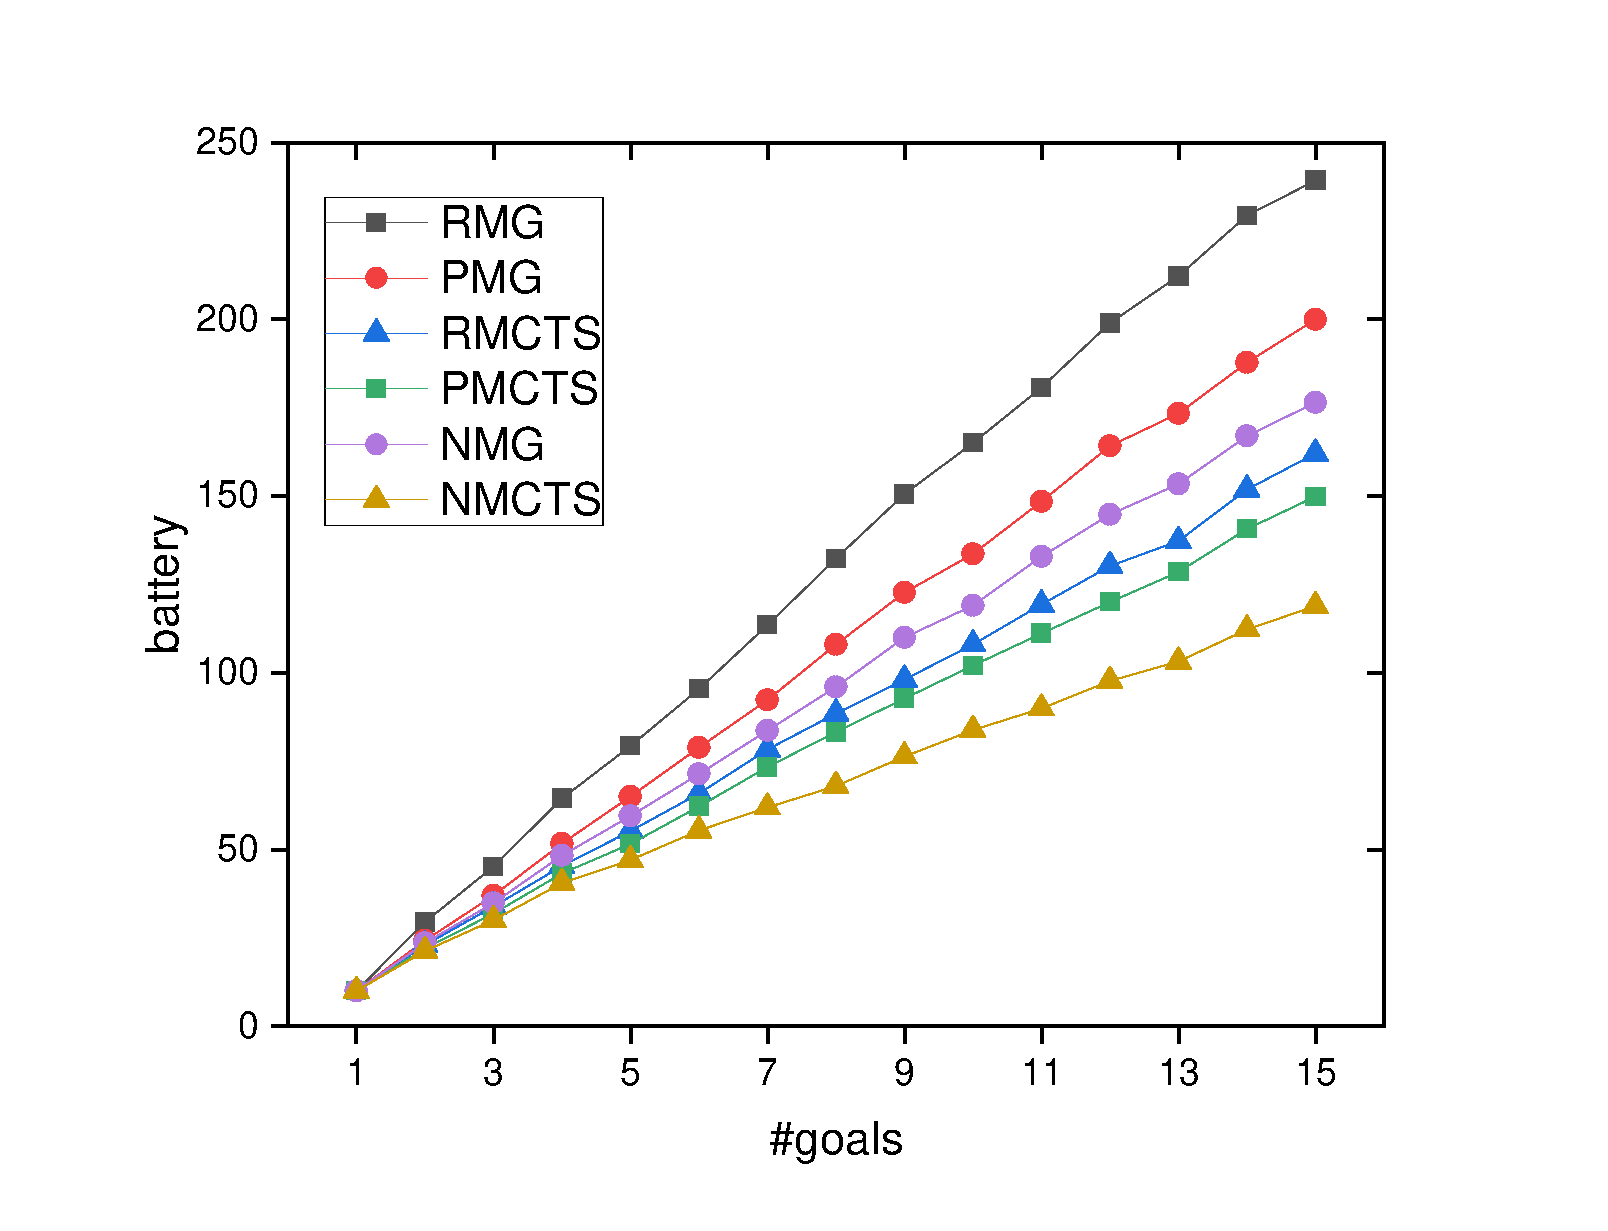
\includegraphics[scale=0.4]{./figs/gX_cY_fixCap40_d}
\captionsetup{justification=centering}
\bicaption{动态环境电池容量为40下的电量消耗}{Battery consumptions with capacity of 40 in dynamic environment}
\label{fig:dynamic1}
\end{figure}

图\ref{fig:dynamic1} 展示了每个方法的平均电量消耗。
%
如图中所见,实验结果与实验一非常类似。
%
NMG,RMG和PMG的性能保持不变,而基于MCTS的方法则有较为明显的性能下降。这是因为即使目标是在不同时间分配的,非MCTS方法的执行规则并没有受到影响,仍然是依次实现给定的目标。但是基于MCTS的方法却无法预测接下来何时会有新目标的分配以及新目标指定的具体位置在何处。基于MCTS的方法只能够基于对环境当前的认知以得出”最优“的决策。
%
然而,相较于其他方法,基于MCTS的方法仍然有显著的性能优势。

\paragraph{实验五}
和实验二类似,在该实验中智能体的电池容量被设定为60,实现目标的数量从1变化至15。另外,$n$的值被设定为5。
具体实验结果如图\ref{fig:dynamic2}所示.
\begin{figure}[h!]
\centering
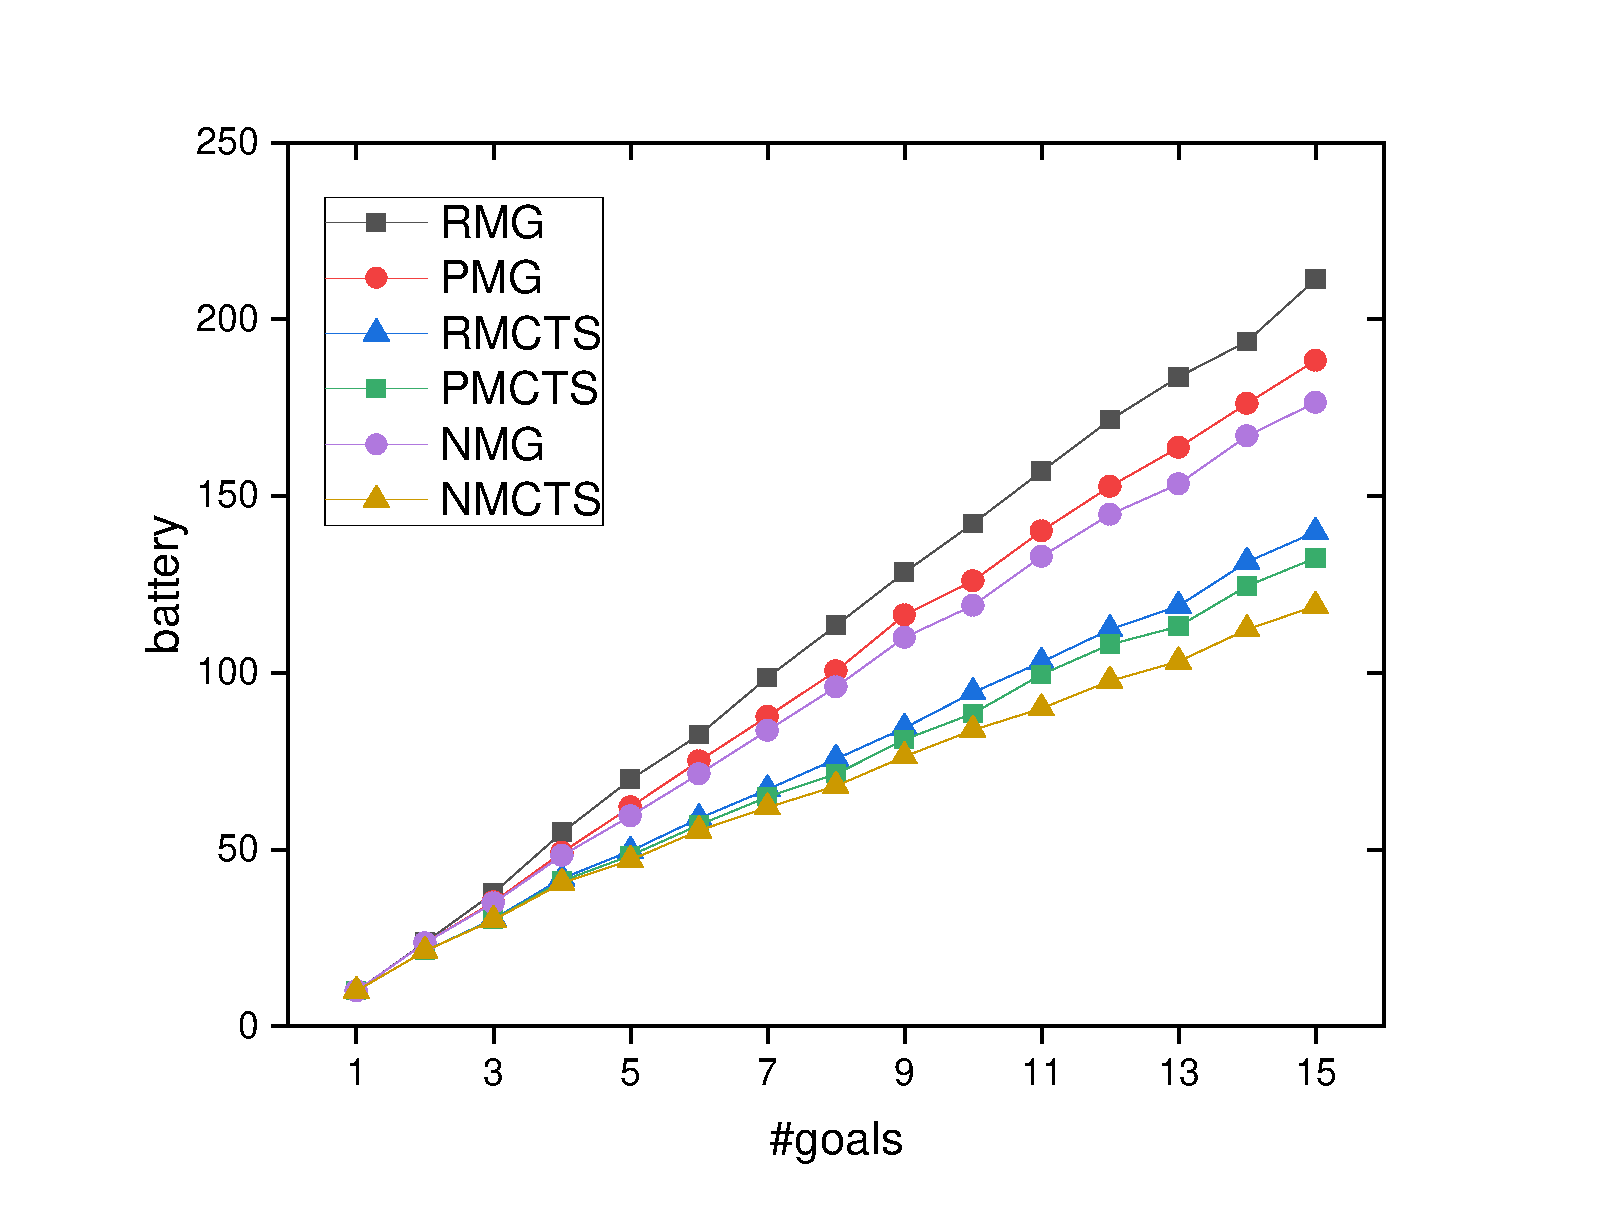
\includegraphics[scale=0.4]{./figs/gX_cY_fixCap60_d}
\captionsetup{justification=centering}
\bicaption{动态环境电池容量为60下的电量消耗}{Battery consumptions with capacity of 60 in dynamic environment}
\label{fig:dynamic2}
\end{figure}

正如所预料的,该实验结果与实验二类似。相较于其他方法,基于MCTS的方法有着显著的性能优势。PMG的表现要优于RMG,但是仍然比基于MCTS的方法要消耗更多的电量,尤其是当实现目标的数量较大时。
%
另外,相较于实验二,基于MCTS的方法间的性能差异有所减小。这是由于在动态环境下智能体需要更多地考虑维持型目标的维护以及修复,导致他们的行为都更趋近于RMCTS,而对于不同意图间协同效应的利用则有所降低。

\paragraph{实验六}
在实验六中,智能体实现目标的数量被固定为10,电池容量被固定为40,分配目标的时间间隔$n$从1改变至15。
\begin{figure}[h!]
\centering
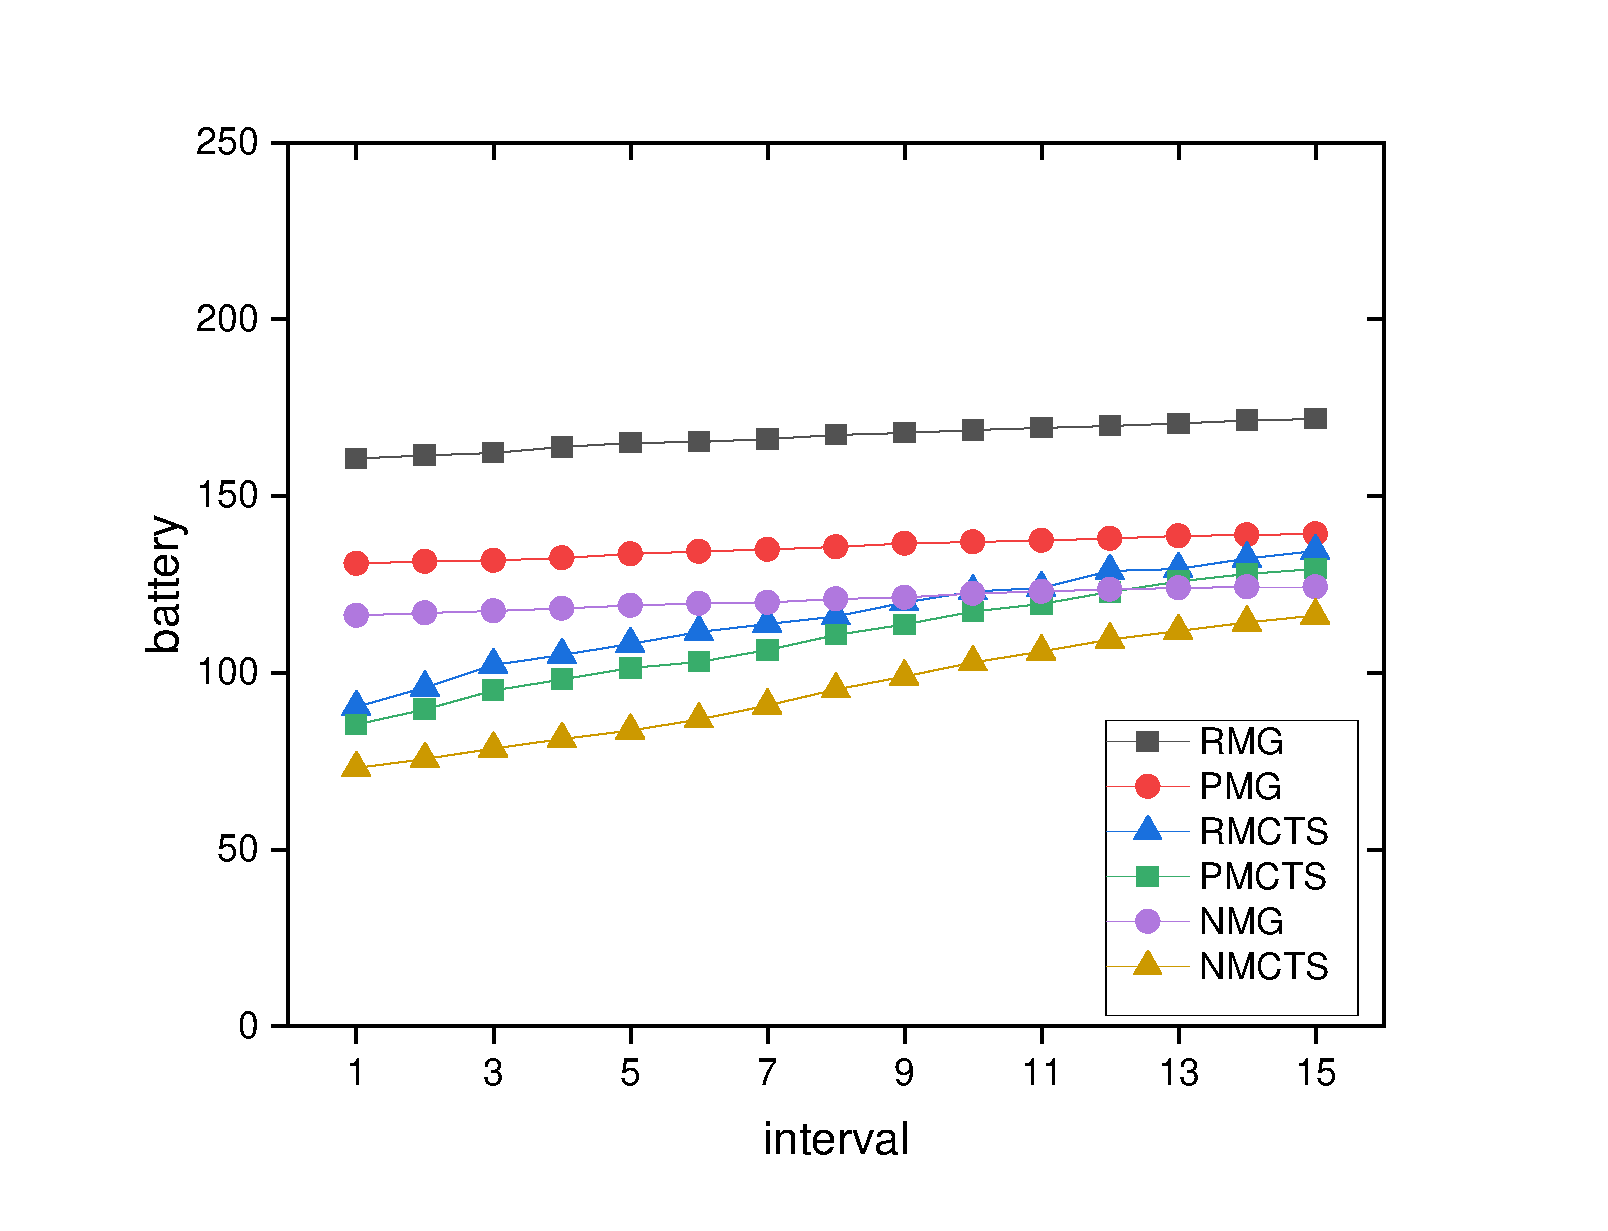
\includegraphics[scale=0.4]{./figs/iX_cY_fixCap40G10}
\captionsetup{justification=centering}
\bicaption{电池容量为40且目标数量为10下的电量消耗}{Battery consumption with capacity of 40 and 10 goals}
\label{fig:dynamic3}
\end{figure}

图\ref{fig:dynamic3}展示了每个方法的平均电量消耗。从图中可得知,基于MCTS方法的性能表现依然要优于其他非MCTS方法。然而,当时间间隔$n$增大时,MCTS是方法的优势越来越低。这是因为当$n$较大时,同时执行的目标数量少,MCTS方法更难以利用不同意图之间的协同效应,致使性能下降;而在$n$较小时,并发执行的意图较多,智能体可以高效利用他们之间的协同效应。当时间间隔被设定为15时,智能体在大多是情况下运行时只有一个目标,因此,MCTS的性能与其他方法非常接近。
\section{本章总结}
本章提出了一种基于\SA 的意图调度算法\SAM 。\SAM 可以同时对实现型和维持型目标进行意图调度。另外,基于火星探测器的模拟场景,本章在静态环境以及动态环境下对\SAM 的性能进行了分析。实验结果表明\SAM 与其他方法(RMG和PMG)相比有着显著的性能优势。即使在没有可靠的预测机制的情况下,\SAM 对被动维持型目标的调度性能表现依旧要优于其他非MCTS方法。\SAM 算法的主要优势有2个:1.避免维持型目标和实现型目标间的相互冲突;2.对多个意图进行交错执行以避免相互冲突并利用其协同效应。

本文的下一章将考虑如何基于\SA,在norm约束场景下对智能体意图进行合理调度。

\chapter{社会规范约束下的意图调度算法}\label{norm}
本章提出一种基于\SA 的意图调度算法\SAN ,\SAN 支持在norm约束下对智能体意图进行调度。和对\SAN 的性能评估方式类似,在实验部分,本研究对\SAN 的性能在动态和静态环境下进行了实验分析,并与Meneguzzi等人提出的v-BDI\cite{DBLP:journals/eaai/MeneguzziROVL15}算法进行了比较,实验结果表明\SAN 的性能相较于v-BDI有显著优势。
\section{社会环境下的norm}
本文的第\ref{mg}章考虑到了社会模拟场景下的维持型目标,提出\SAM 算法对智能体的实现型目标和维持型目标进行调度。在本章中,社会模拟场景下的norm为主要考虑对象。

第\ref{background}章中提到在社会场景下,norm是一种重要的管控智能体行为的手段\cite{DBLP:journals/mags/SavarimuthuC11}。有三种类型的norm,一种是义务,其定义了智能体应当做什么;另一种是许可,其定义了智能体可以做什么;最后一种是禁令,其定义了智能体被禁止做什么。本文主要考虑的禁令类型的norm以及其如何影响智能体的行为。

现有对IPP的研究往往忽略了智能体在社会场景下执行的情况。其假设只要动作的前置条件满足,智能体即可执行。另外,智能体的性能表现也是基于目标完成数量进行评估的。然而在社会场景中,智能体的行为可能会受到norm的约束以确保智能体的正常运行。例如,在火星探测器场景下,智能体可能被禁止前往陡峭的高坡以避免跌落受到损害。

% survey
% logic based
正如第\ref{background}章中所提到的,在BDI智能体研究领域,为了解决norm约束下的意图进展问题,可以像BOID\cite{DBLP:conf/agents/BroersenDHHT01}、NBM\cite{DBLP:conf/atal/MeneguzziL09}以及NoA\cite{DBLP:conf/ijcai/KollingbaumN03}一样,基于逻辑规则对智能体的行为进行限制,在智能体运行时严格遵守逻辑规则避免对norm的违反。然而,这类方法极大程度地限制了智能体的灵活性,在某些情况下智能体需要违反norm以实现更重要的目标。例如,破坏窗户的行为是norm禁止的,但是当发生火灾时,一个理性的智能体应该为了逃生而破坏窗户离开火灾区域。另外,这类方法需要用户自定义逻辑规则。当应用于复杂环境时,用户需要编写大量规则,这加重了用户负担并且可能由于规则数量庞大导致智能体程序进行逻辑解析的计算开销增大,加重决策负担。
% priority based
N-2APL\cite{DBLP:conf/aamas/AlechinaDL12}和N-Jason\cite{DBLP:conf/dalt/LeePLDA14}使用优先级的概念对不同的目标、norm进行划分。相较于存粹的逻辑规则而言,基于优先级的方法有着更强的灵活性,但是仍然对用户的负担较大(优先级规则由用户自定义),且由于原子计划的设定(原子计划的执行无法被打断),其无法高效利用不同意图间的协同效应。
% value based
基于价值评估的v-BDI\cite{DBLP:journals/eaai/MeneguzziROVL15}在计划选择时对可执行计划进行价值评估,最终选择价值最高的计划执行。若完成计划的收益大于违反相关norm的惩罚,智能体可以选择违反norm已获得更高的综合收益。使用该方法,用户仅仅需要定义价值评估函数即可,这大幅度减轻了用户的负担。然而v-BDI的一个明显的劣势在于其没有考虑到意图之间的交互。在进行意图选择时v-BDI遵循FIFO的规则。

本章考虑在norm约束下对智能体意图的调度,\SAN 算法允许智能体做出违反norm的行为已获得更大收益,提高了智能体的灵活性;另一方面,\SAN 仅需要用户提供价值评估函数即可,这减轻了用户的负担;最后,\SAN 可以高效利用不同意图间的协同效应,显著提升智能体的性能表现。

\section{norm的表示与问题定义}
% Formal representation.
一个(禁令类型)norm被规范表示为一个三元组:
$$<C,A,R>$$
其中,
\begin{itemize}
  \item $C$ 为一组命题公式,表示该norm的触发条件;
  \item $A$ 为该norm的目标动作;
  \item $R$ 为一个数值,表示当智能体违反norm时收到的惩罚。
\end{itemize}

根据该定义,当给定一个norm $N=<C,A,R>$时,若智能体执行动作$A$,且其当前所处环境下满足$C$,那么智能体违反该norm,并受到$R$数值的惩罚。

本章对IPP的原始定义进行扩展,加入norm的限制,使得智能体必须同时考虑目标(如何实现目标)以及norm(如何避免违反norm)。本章基于效用函数对智能体的性能进行评估,该效用函数将实现目标的相关性能(如实现目标的数量,消耗的资源等)与违反norm而受到的惩罚值作为参数。

具体地,基于目标计划树模型,norm约束下的智能体意图调度问题可被定义为:给定一组表示智能体意图的目标计划树$\{t_1, \dots, t_n\}$以及一组表示智能体当前环境状态的条件变量$Env$,在每一个执行周期中返回一个目标计划树$t_i$中的下一个执行步骤使得智能体实现的目标数量最多,因违反norm受到的惩罚最小且消耗的资源最少。

\section{\SAN 意图调度算法}
本章介绍norm约束下的意图调度算法\SAN,\SAN 在第\SA (已在第\ref{SA}章中介绍)的基础上进行拓展,加入对norm考虑。
\SAN 算法修改了\SA 算法中的扩展与模拟阶段,加入了对因违反norm而受到惩罚的模拟,以下是对SA算法的具体修改细节:
\paragraph{对扩展阶段的修改}
% Reactive
在扩展阶段,\SAN 首先检查某个选中的叶子节点$n_s$状态下每一个可执行动作$a_i$,若$a_i$不会违反norm,则直接生成一个新的节点对应于执行$a_i$的结果,并作为$N_s$的一个孩子节点。若$a_i$会违反norm,则首先进行如下检查:检查$a_i$所在意图$t_i$,若$t_i$所实现目标$g_i$的价值$V_i$大于当前执行$t_i$所受到的总惩罚值$P_i$(包括执行$a_i$的惩罚值),则生成一个新节点对应于执行$a_i$的结果。相反,若$t_i$所实现目标$g_i$的价值$V_i$小于当前执行$t_i$所受到的总惩罚值$P_i$,则不生成新的节点。
%
当所有可执行动作$a_i$都会造成$P_i > V_i$时,则不会有新的节点生成。该情况下智能体会暂停其执行。
%
在\SAN 中,每个节点记录的信息除智能体意图、环境状态外,还记录了执行过程中所收到的总惩罚值以及执行每个意图所受到的部分惩罚值。

\paragraph{对模拟阶段的修改}
在模拟阶段,\SAN 和\SA 一样,随机选择实现目标过程中可执行的动作执行。当某个可执行动作$a_i$违反norm时,进行如下检查:检查$a_i$所在意图$t_i$,若$t_i$所实现目标$g_i$的价值$V_i$大于当前执行$t_i$所受到的总惩罚值$P_i$(包括执行$a_i$的惩罚值),则禁止该动作的执行。相反,若$t_i$所实现目标$g_i$的价值$V_i$小于当前执行$t_i$所受到的总惩罚值$P_i$,则直接执行。

当以下三个条件中的任意一个满足时,模拟阶段即停止:
\begin{enumerate}
  \item 所有的目标都已实现。
  \item 当前状态下无法实现剩余的实现型目标。
  \item 所有的可执行动作$a_i$都会导致其所在意图$T_i$当前的总惩罚值$P_i$ 大于 $T_i$所实现的目标价值$V_i$。
\end{enumerate}

\section{实验}
\subsection{实验场景介绍}
本章的实验场景与上一章类似,基于火星探测器的模拟场景(见图\ref{fig:marsrover})。不同的是在考虑norm的情况下,本实验假设智能体所处的地表并非完全平坦:在不同的方格直接可能存在一定的高低差,出现斜坡。这些斜坡可能对智能体的行动造成影响。对于智能体来说,跨越这些斜坡是非常危险的,可能会造成智能体机械结构的损伤(但是智能体仍然可以选择冒险跨越斜坡)。因此,本实验设定如果智能体跨越斜坡就会违反norm并受到相应的惩罚值。在以下实验中,为了专注于探究norm对智能体决策的影响,假设智能体拥有无限的电池容量,而无需考虑返回基地充电(电量消耗仍然为评估标准之一,如此设定仅为了让智能体无需考虑电量相关的维持型目标)。

% measring the agent performance
本实验根据三个指标对智能体的性能进行评估:完成目标的数量、电池消耗量以及总惩罚值。具体地,本实验根据评估函数$\frac{\#goals}{batteryConsumption} - penaltyValue$对智能体的性能进行评估,其中$\#goals$为实现目标的数量,$batteryConsumption$为电池消耗量,$penaltyValue$为因违反norm而受到的总惩罚值。该价值函数决定了智能体的综合性能表现。另外,实验中每个norm的惩罚值随机生成,随机生成的惩罚值符合正态分布$\sigma(0.1, 0.01)$

本文将\SAN 与Meneguzzi等人提出的v-BDI\cite{DBLP:journals/eaai/MeneguzziROVL15}进行比较。如第\ref{background}中所提到,v-BDI以FIFO的规则进行意图选择,在计划选择阶段则选择价值最大的计划执行。具体地,v-BDI在做出计划选择之前对每个可应用计划进行评估,评估检查计划所实现的目标具有多少收益,以及计划中的动作是否会违反norm,以及如果执行这些动作会造成多少惩罚。然后基于用户自定的效用函数对每个计划进行综合评价得出计划价值。

在接下来的实验中,v-BDI的价值函数被设定为$\frac{\#goals}{batteryConsumption} - penaltyValue$。\SAN 算法设定为执行100次迭代($\alpha = 100$),每次迭代执行10次的模拟($\beta = 10$)。\SAN 的价值函数与v-BDI相同,设定为$\frac{\#goals}{batteryConsumption} - penaltyValue$。

与上一章中的实验类似,本章实验考虑了动态与静态环境。以下的实验结果展示的是每种方法运行100次运行次的平均性能。另外,实际上所有方法都可以在实验中实现所有顶层目标。因此,为了便于分析,本实验结果分析中不以完成目标数量为标准对智能体性能进行比较。

本实验将\SAN 与v-BDI进行对比。另外,NMG(介绍于第\ref{mg}章实验部分)在本实验中作为基准用于评估\SAN 和v-BDI的性能。
在以下实验的结果图中,NMG以FIFO所标注,\SAN 以MCTS标注。
\subsection{静态环境实验}
接下来的三个实验考虑火星探测器智能体在静态环境下的表现。在静态环境下,智能体的所有实现型目标都在初始运行时给定。
\paragraph{实验一}
在第一个实验中,norm的数量被设定为10,智能体需要实现的目标数量从1逐步增加至15。具体实验结果如图\ref{fig:all_fixNorms10}所示。

\begin{figure}
\centering
\begin{subfigure}{.47\textwidth}
  \centering
  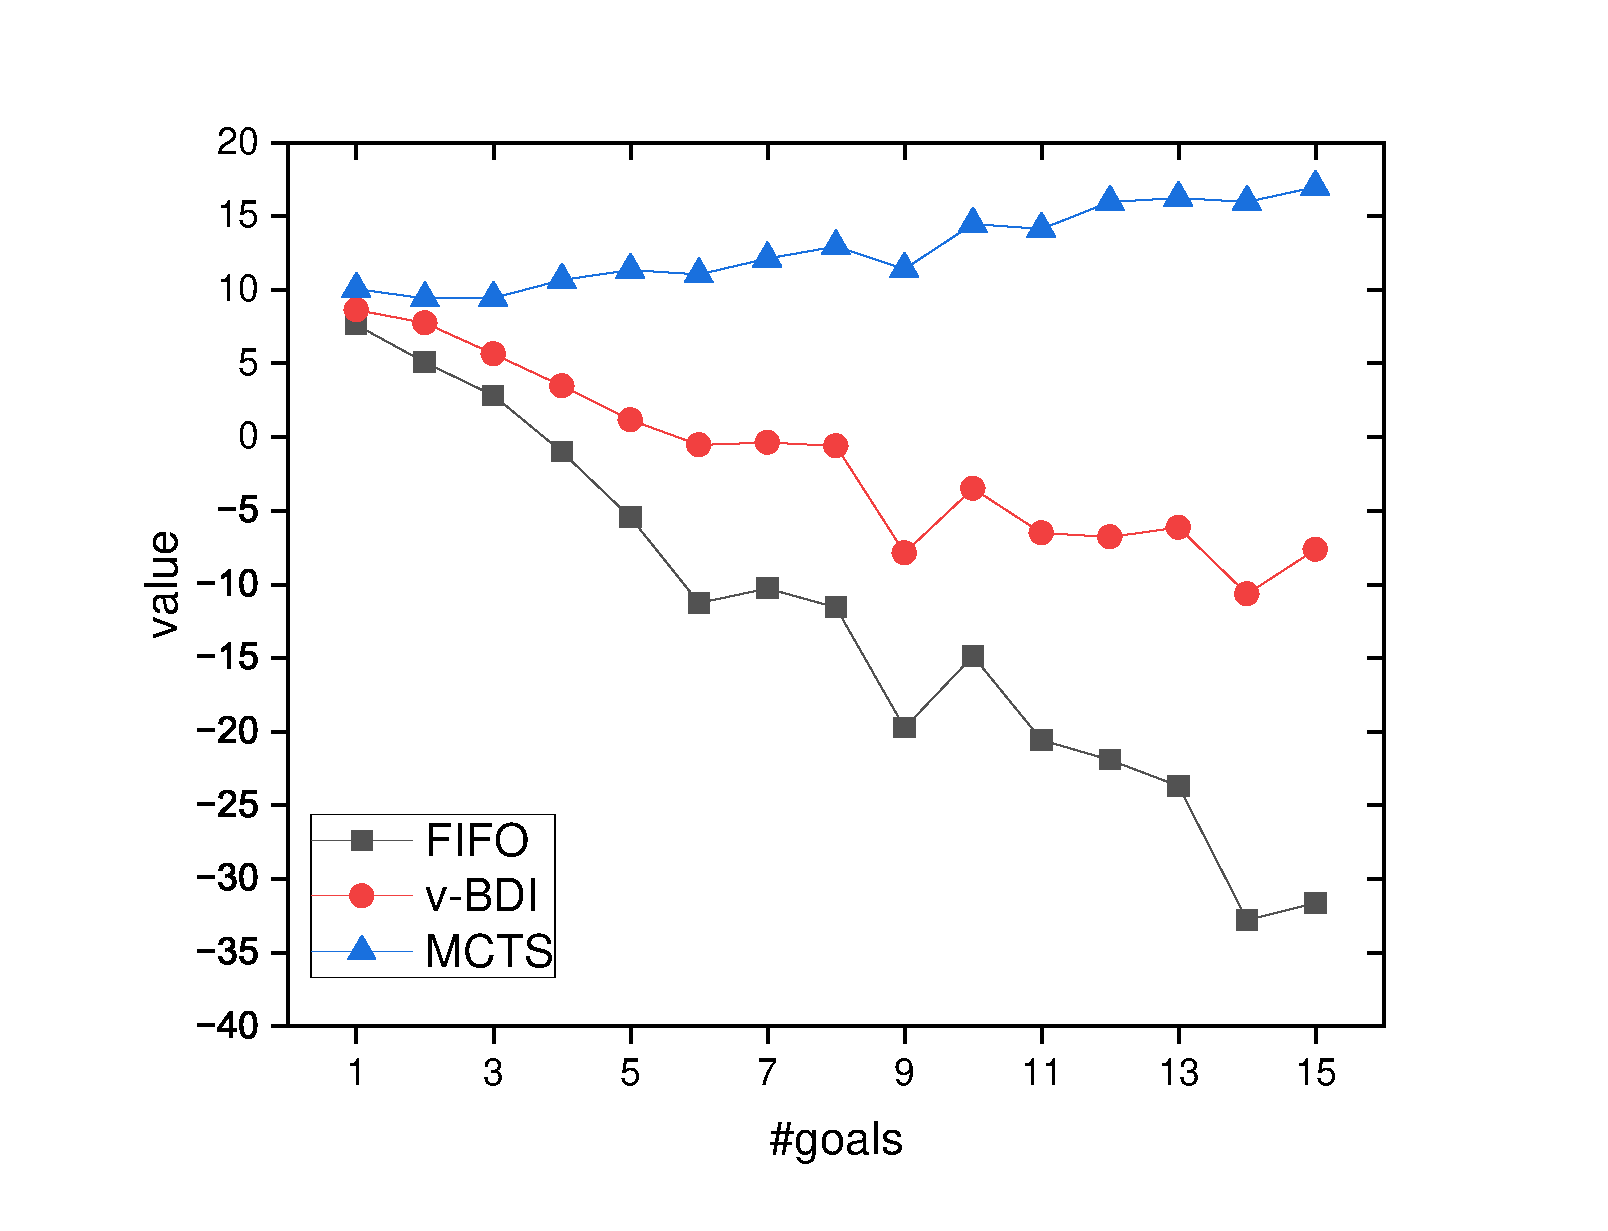
\includegraphics[scale=0.18]{goalsX_valueY_fixNorms10.pdf}
  \captionsetup{justification=centering}
  \caption{Utility}
  \label{fig:goalsX_valueY_fixNorms10}
\end{subfigure}

\begin{subfigure}{.47\textwidth}
  \centering
  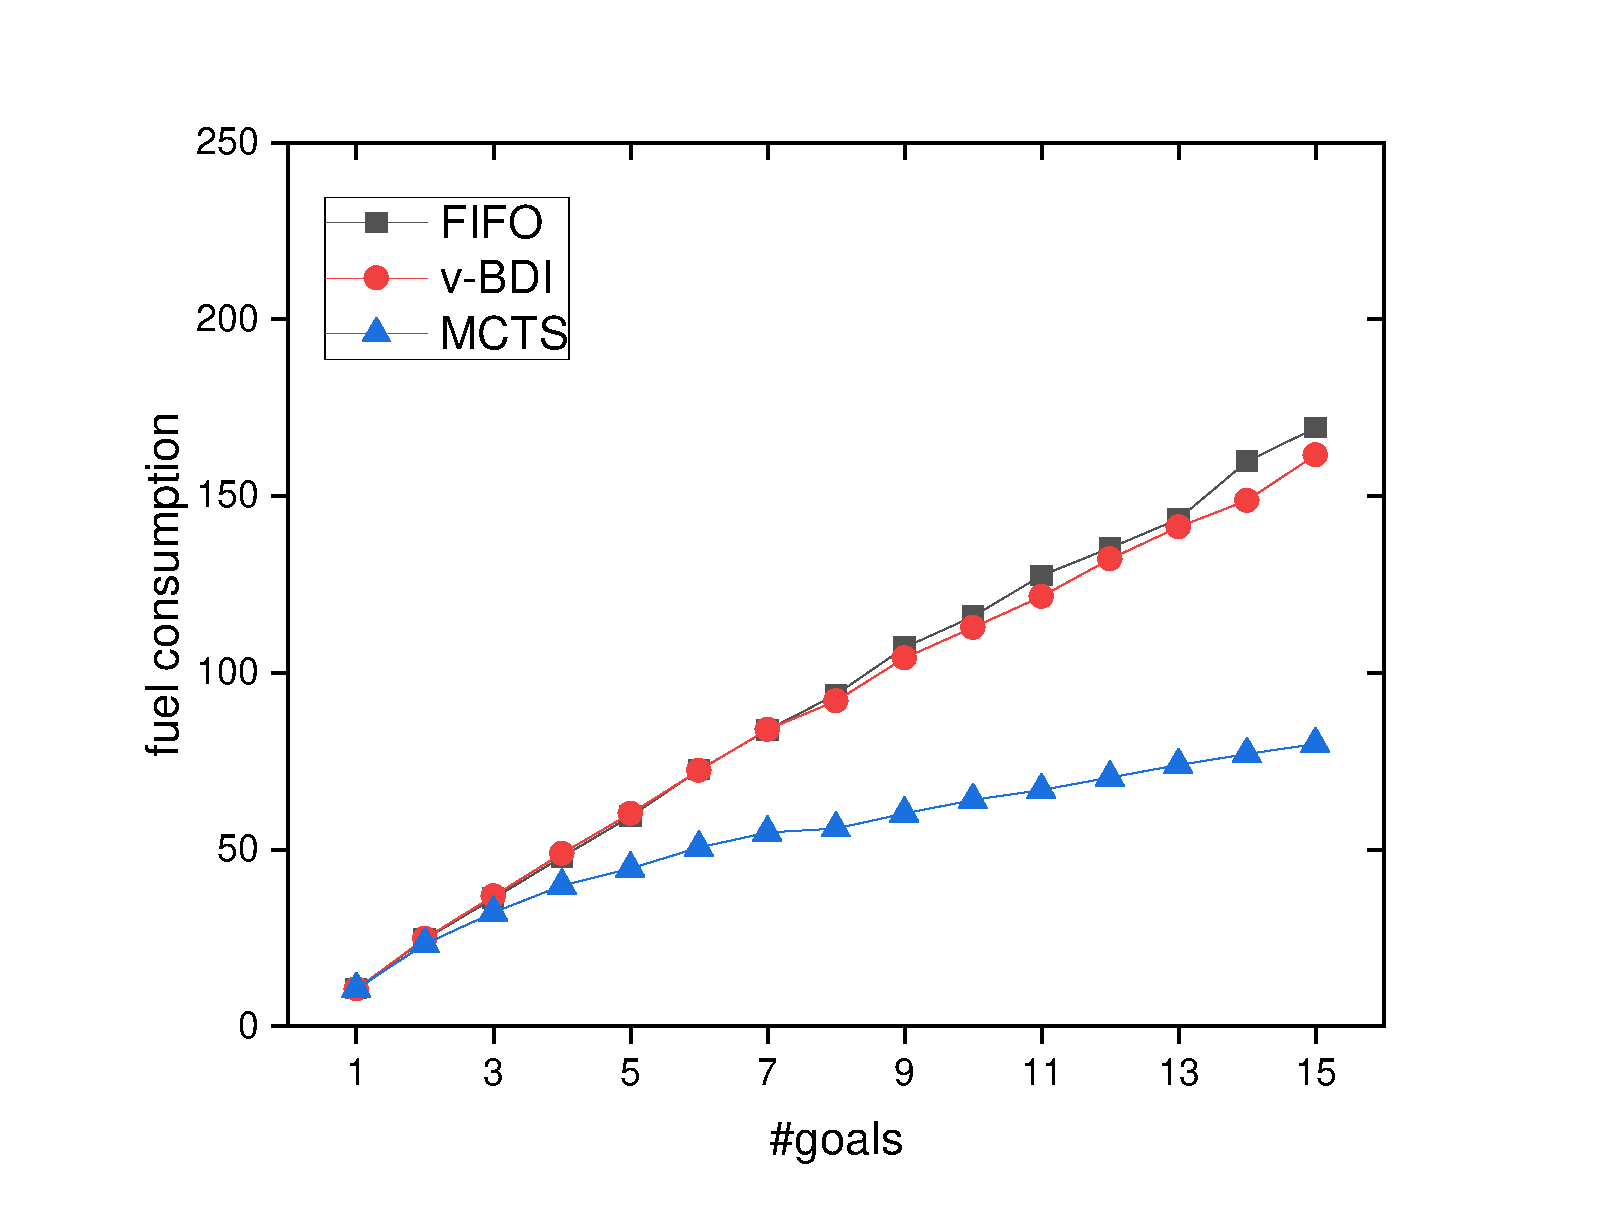
\includegraphics[scale=0.18]{goalsX_consumptionY_fixNorms10.pdf}
  \captionsetup{justification=centering}
  \caption{Fuel consumption}
  \label{fig:goalsX_consumptionY_fixNorms10}
\end{subfigure}
\begin{subfigure}{.47\textwidth}
  \centering
  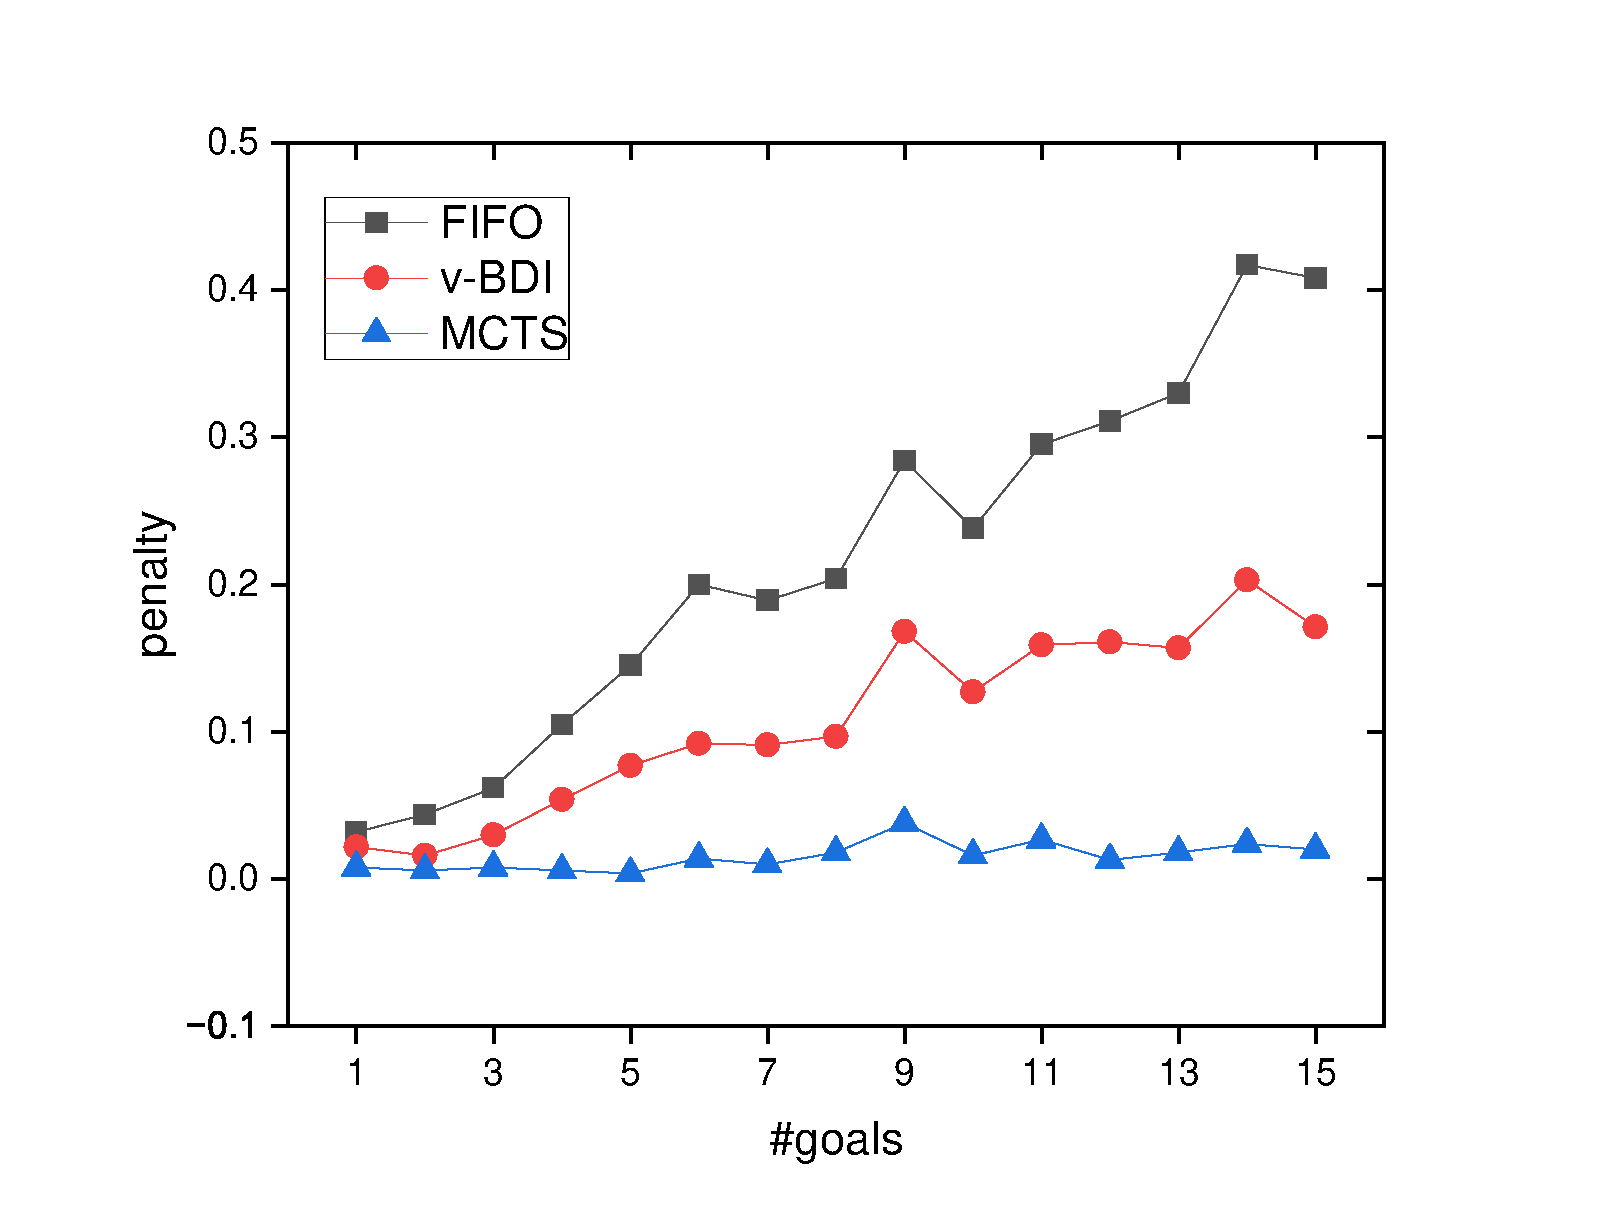
\includegraphics[scale=0.18]{goalsX_penaltyY_fixNorms10.pdf}
  \captionsetup{justification=centering}
  \caption{Penalty}
  \label{fig:goalsX_penaltyY_fixNorms10}
\end{subfigure}
\captionsetup{justification=centering}
\bicaption{norm数量为10下的实验结果}{Overall utility, fuel consumption and penalty with fixed \#norms 10}
\label{fig:all_fixNorms10}
\end{figure}

\paragraph{总价值分析}
% Note fifo
从图中可知,当实现目标数量增加时,NMG与v-BDI的总价值降低。NMG在所有情况下的性能表现都最差。
% Reason
这是因为NMG不考虑norm的影响,且忽略了不同意图之间可能出现的负面影响以及协同效应,导致性能表现低下。
% v-BDI performance
v-BDI具有比NMG更好的性能表现,因为其可以评估执行计划导致违反norm的惩罚值。v-BDI始终选择效用值最高的计划执行,从而比NMG违反更少的norm,导致最终获得更高的总价值。
% MCTS performance
最后,正如图中所示,MCTS(即\SAN 算法)有相比于NMG和v-BDI有着明显的性能优势。特别是当给定目标数量多时,MCTS与其他方法直接的差异更为显著。这是因为MCTS可以在决策时考虑到norm的影响,并且高效利用不同意图间的协同效应,通过合并不同意图间的相同动作以减少执行次数。这使得智能体有更低的可能性违反norm。与NMG、v-BDI不同,当目标数量增加时,MCTS的性能甚至略有增加(在某些部分)。这是因为在norm的数量较少的情况下(10个norm),目标数量增加时,MCTS可以更好地利用意图间的协同效应,而该协同效应带来的优势克服了违反norm的次数增加带来的危害,从而产生了更高的总价值。然而在后续实验中可以看到,当norm数量较多时,违反norm的危害很难被协同效应所克服。

% Penalty and consumption
\paragraph{电量消耗分析}
% Consumption
如图\ref{fig:goalsX_consumptionY_fixNorms10}所示, 随着目标数量的增加,所有方法的电量消耗都有所增加。与NMG和v-BDI相比,MCTS消耗的电量最少。这是由于MCTS利用意图间的协同效应节省了大量执行步骤。而NMG与v-BDI在意图选择是都遵守FIFO策略,导致执行步骤更多,造成电量的浪费。
\paragraph{惩罚值分析}
% Penalty
如图\ref{fig:goalsX_penaltyY_fixNorms10}所示, v-BDI受到的惩罚值比NMG低。这是由于v-BDI在计划选择时会有意地避免违反norm的计划,导致违反norm的次数更少。最后,相比于NMG和v-BDI,MCTS有着显著的性能优势。特别是当给定目标的数量较大时,MCTS与其他两种方法的差距更明显。

\paragraph{实验二}
在第二个实验中,norm的数量被改变为30,其他实验设置参数与实验一相同。图\ref{fig:all_fixNorms30}展示了实验结果。

\begin{figure}
\centering
\begin{subfigure}{.47\textwidth}
  \centering
  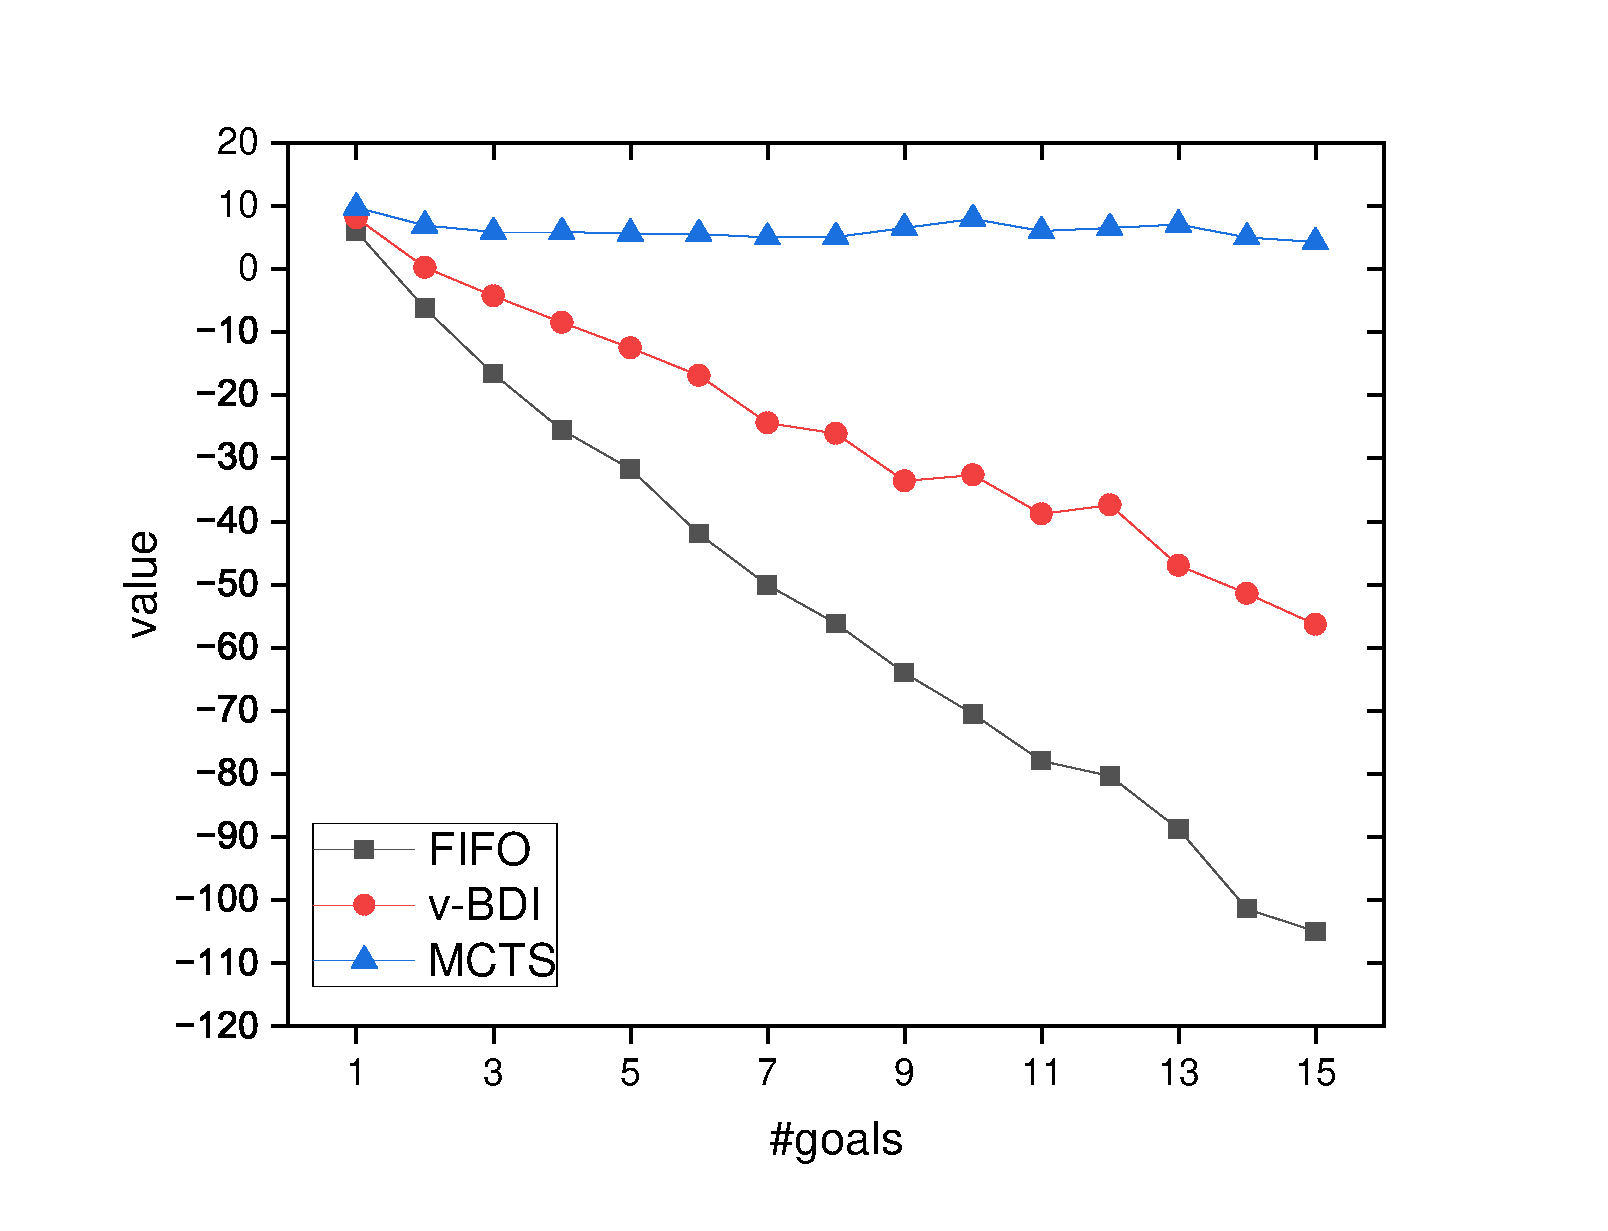
\includegraphics[scale=0.18]{goalsX_valueY_fixNorms30.pdf}
  \captionsetup{justification=centering}
  \caption{Utility}
  \label{fig:goalsX_valueY_fixNorms30}
\end{subfigure}

\begin{subfigure}{.47\textwidth}
  \centering
  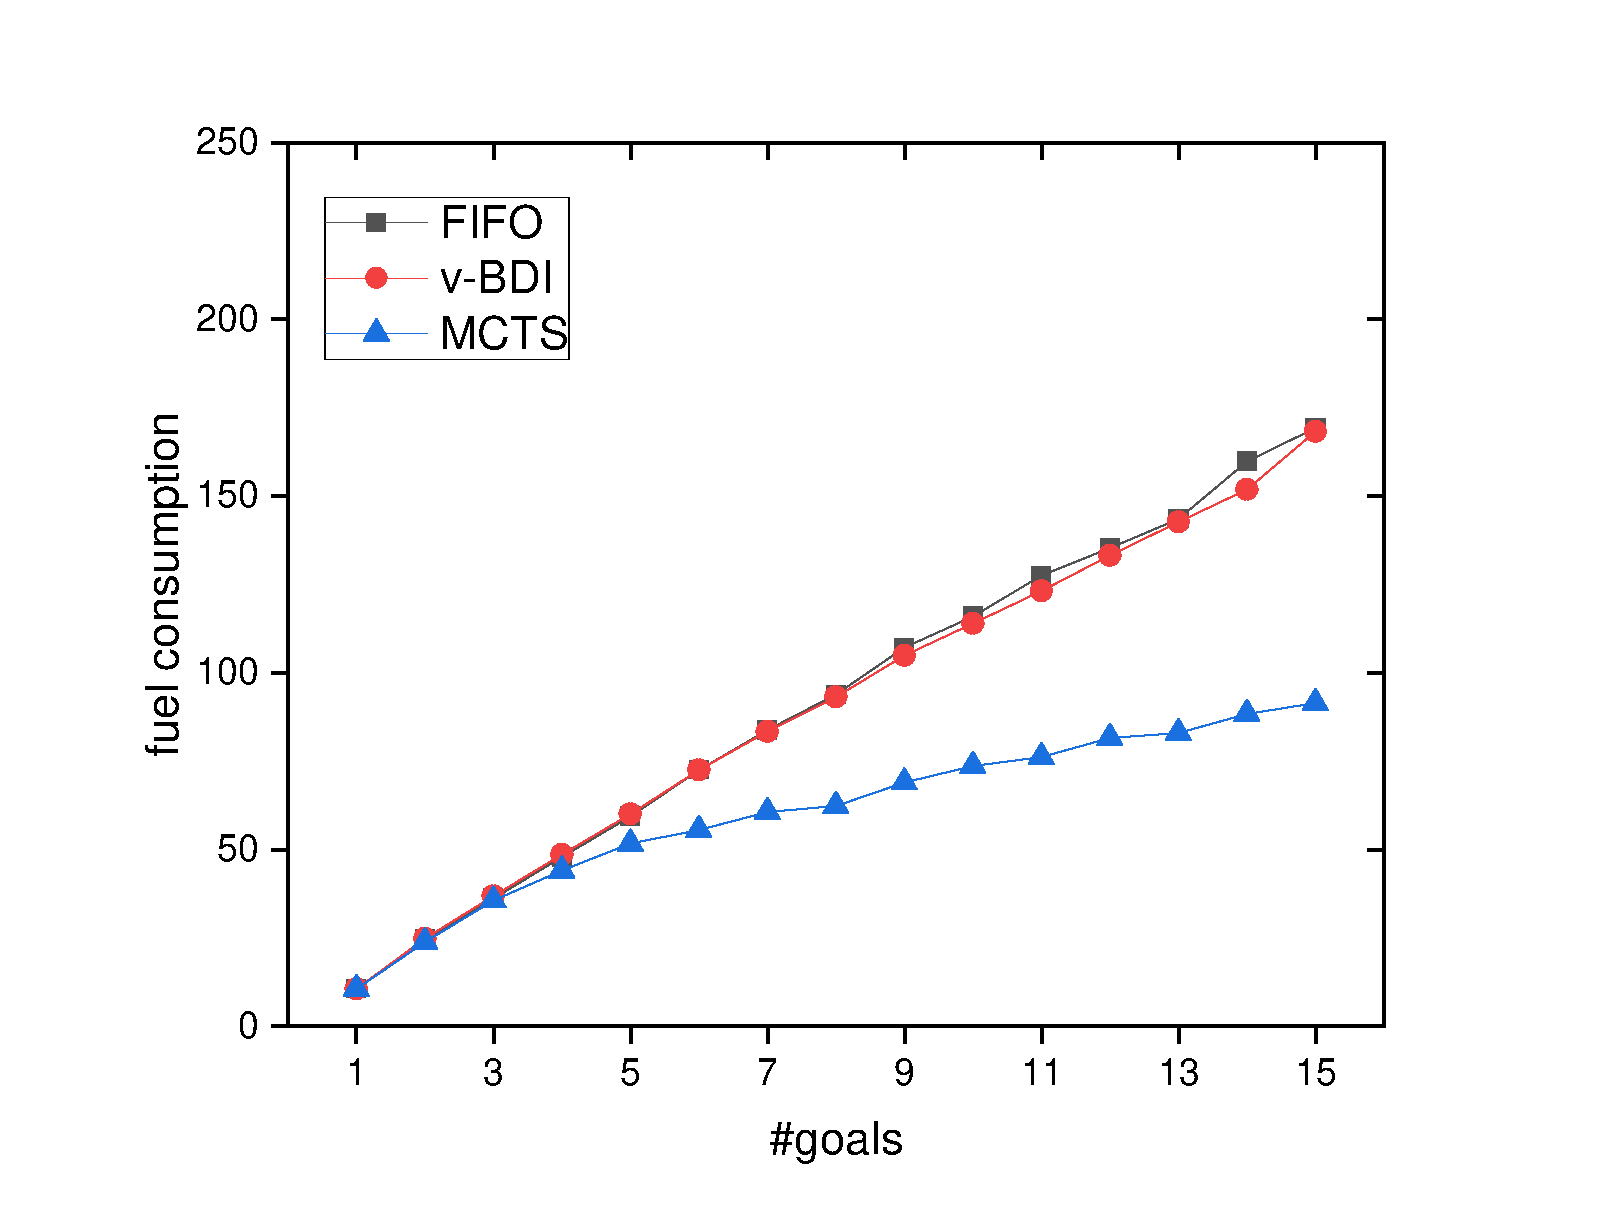
\includegraphics[scale=0.18]{goalsX_consumptionY_fixNorms30.pdf}
  \captionsetup{justification=centering}
  \caption{Fuel consumption}
  \label{fig:goalsX_consumptionY_fixNorms30}
\end{subfigure}
\begin{subfigure}{.47\textwidth}
  \centering
  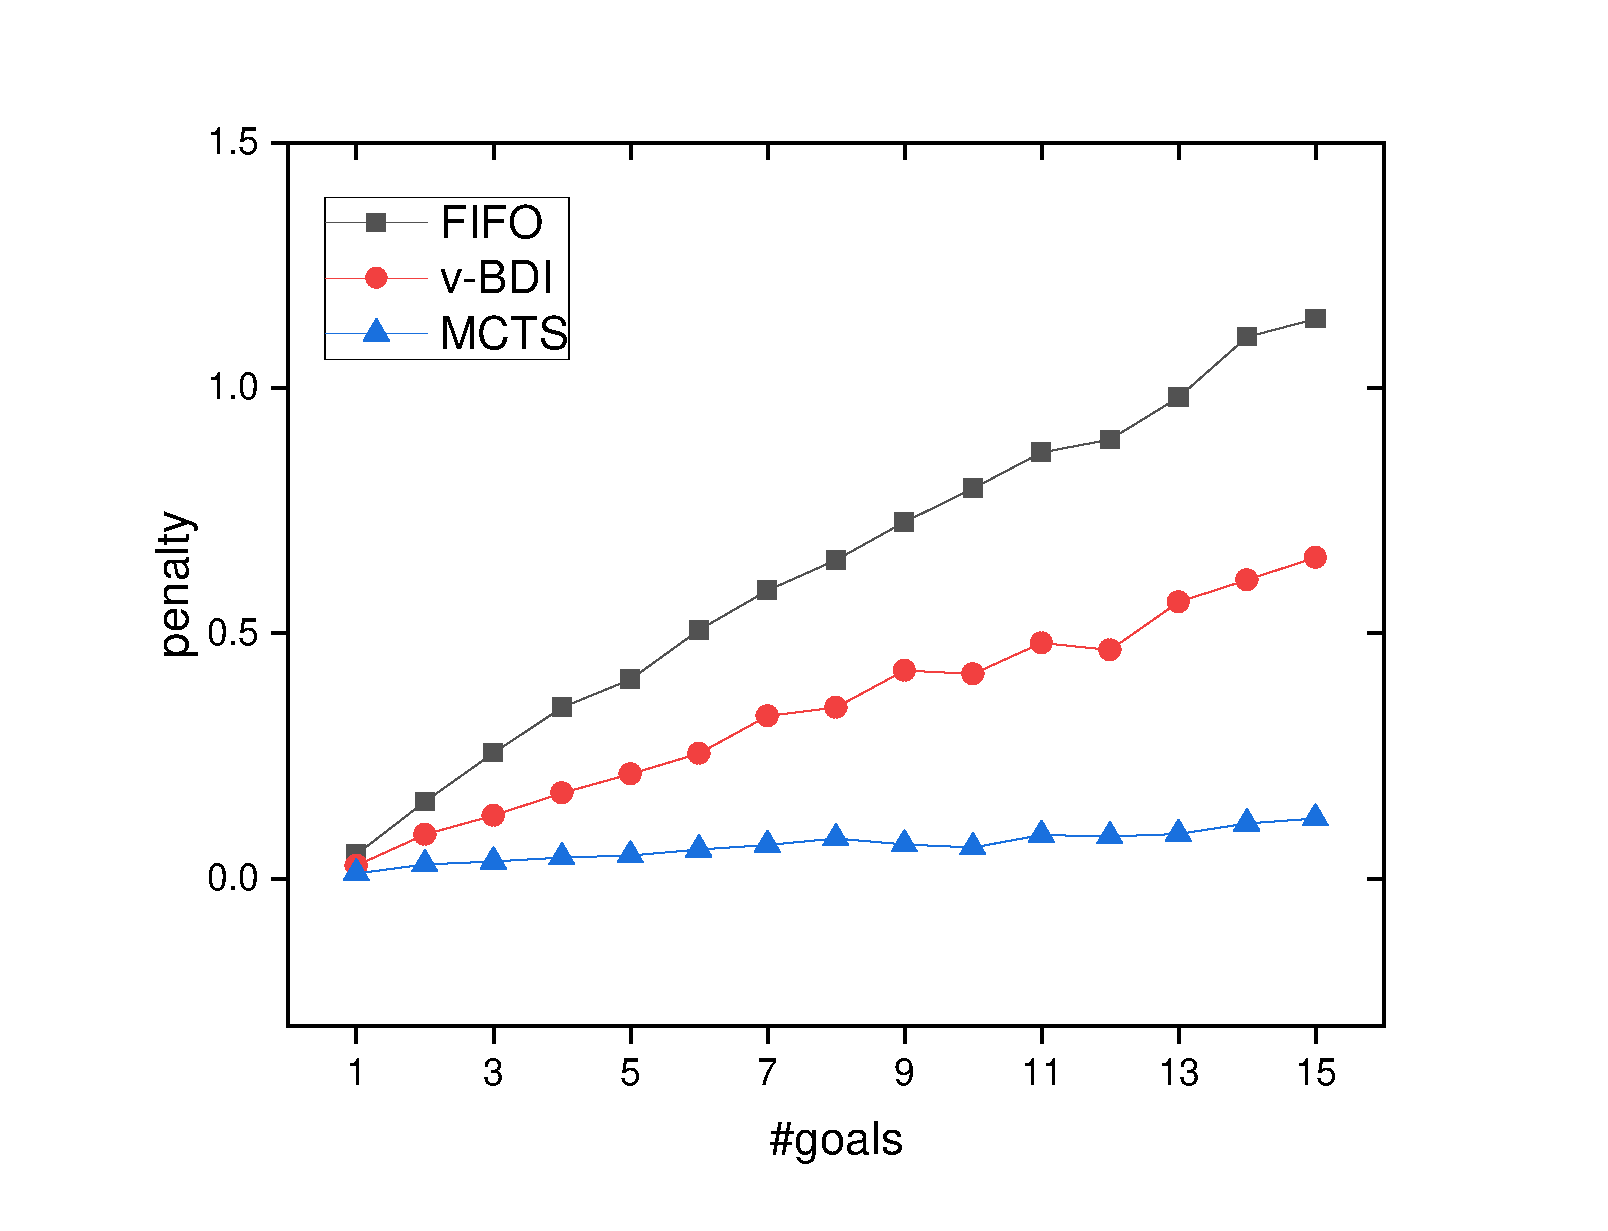
\includegraphics[scale=0.18]{goalsX_penaltyY_fixNorms30.pdf}
  \captionsetup{justification=centering}
  \caption{Penalty}
  \label{fig:goalsX_penaltyY_fixNorms30}
\end{subfigure}
\captionsetup{justification=centering}
\bicaption{norm数量为10下的实验结果}{Overall utility, fuel consumption and penalty with fixed \#norms 30}
\label{fig:all_fixNorms30}
\end{figure}

% Figure information
如图\ref{fig:goalsX_valueY_fixNorms30}所示,当实现目标数量增加时,NMG与v-BDI的性能表现明显下降。MCTS方法依然保持最高的性能表现,且几乎没有下降趋势。

% MCTS performance
然而与上一个实验相比,MCTS的性能表现有所下降。
% Reason
这是因为在当前实验中,norm的数量较多,对多目标间协同效应的利用带来的收益几乎无法抵消违反norm带来的惩罚。此外,与实验一相比,图中所示的三种方法性能表现更为稳定,这是因为当norm数量较多时,在环境中的分布更为均匀。
% Consumption
如图\ref{fig:goalsX_consumptionY_fixNorms30}所示,三种方法的电量消耗与实验一几乎相同,这是因为目标位置并没有发生变化,因此智能体需要移动的距离不会改变。
% Penalty
如图\ref{fig:goalsX_penaltyY_fixNorms30}所示, 所有方法受到的惩罚值相较于实验一都有提升。然而MCTS方法的性能表现依旧强于NMG和v-BDI。

\paragraph{实验三}
在第三个实验中,智能体被给定固定10个目标,而norm的数量从0改变至50。具体实验结果如图\ref{fig:all_fixGoals10}所示。

\begin{figure}
\centering
\begin{subfigure}{.47\textwidth}
\centering
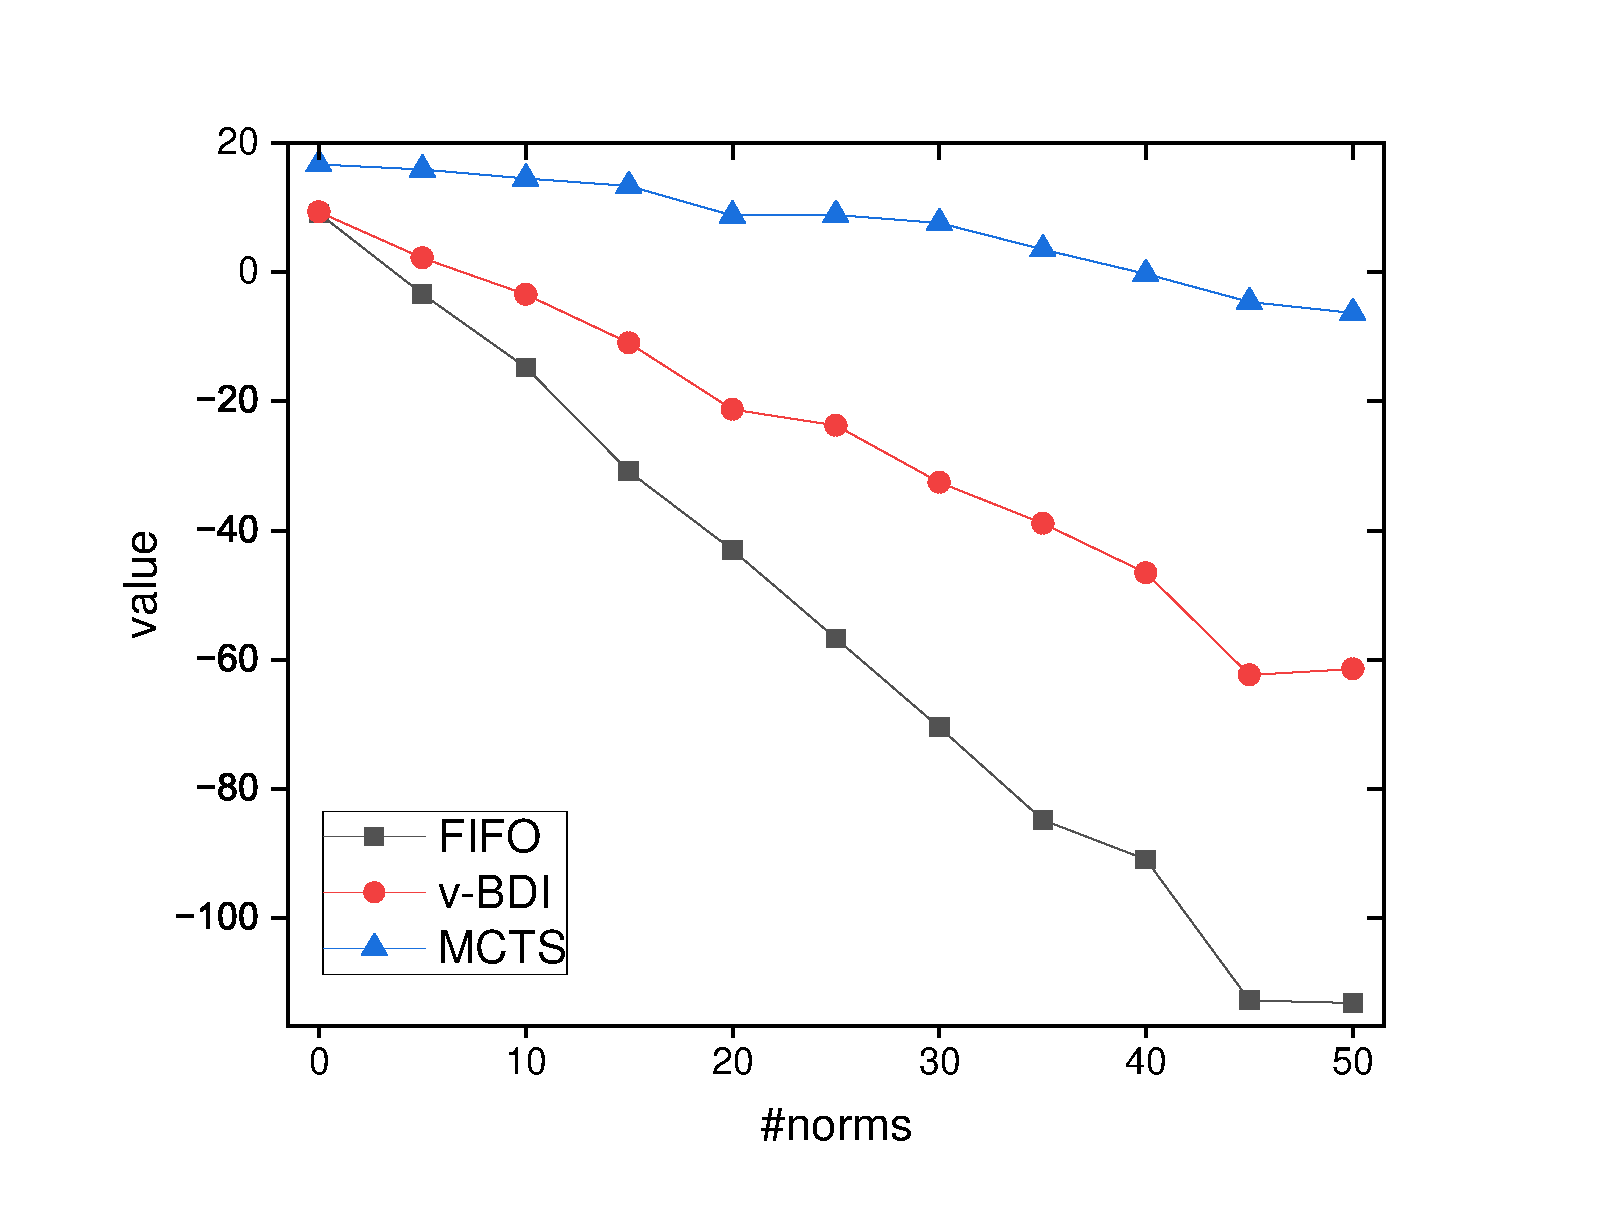
\includegraphics[scale=0.18]{normsX_valueY_fixGoals10.pdf}
\captionsetup{justification=centering}
\caption{Utility}
\label{fig:normsX_valueY_fixGoals10}
\end{subfigure}

\begin{subfigure}{.47\textwidth}
  \centering
  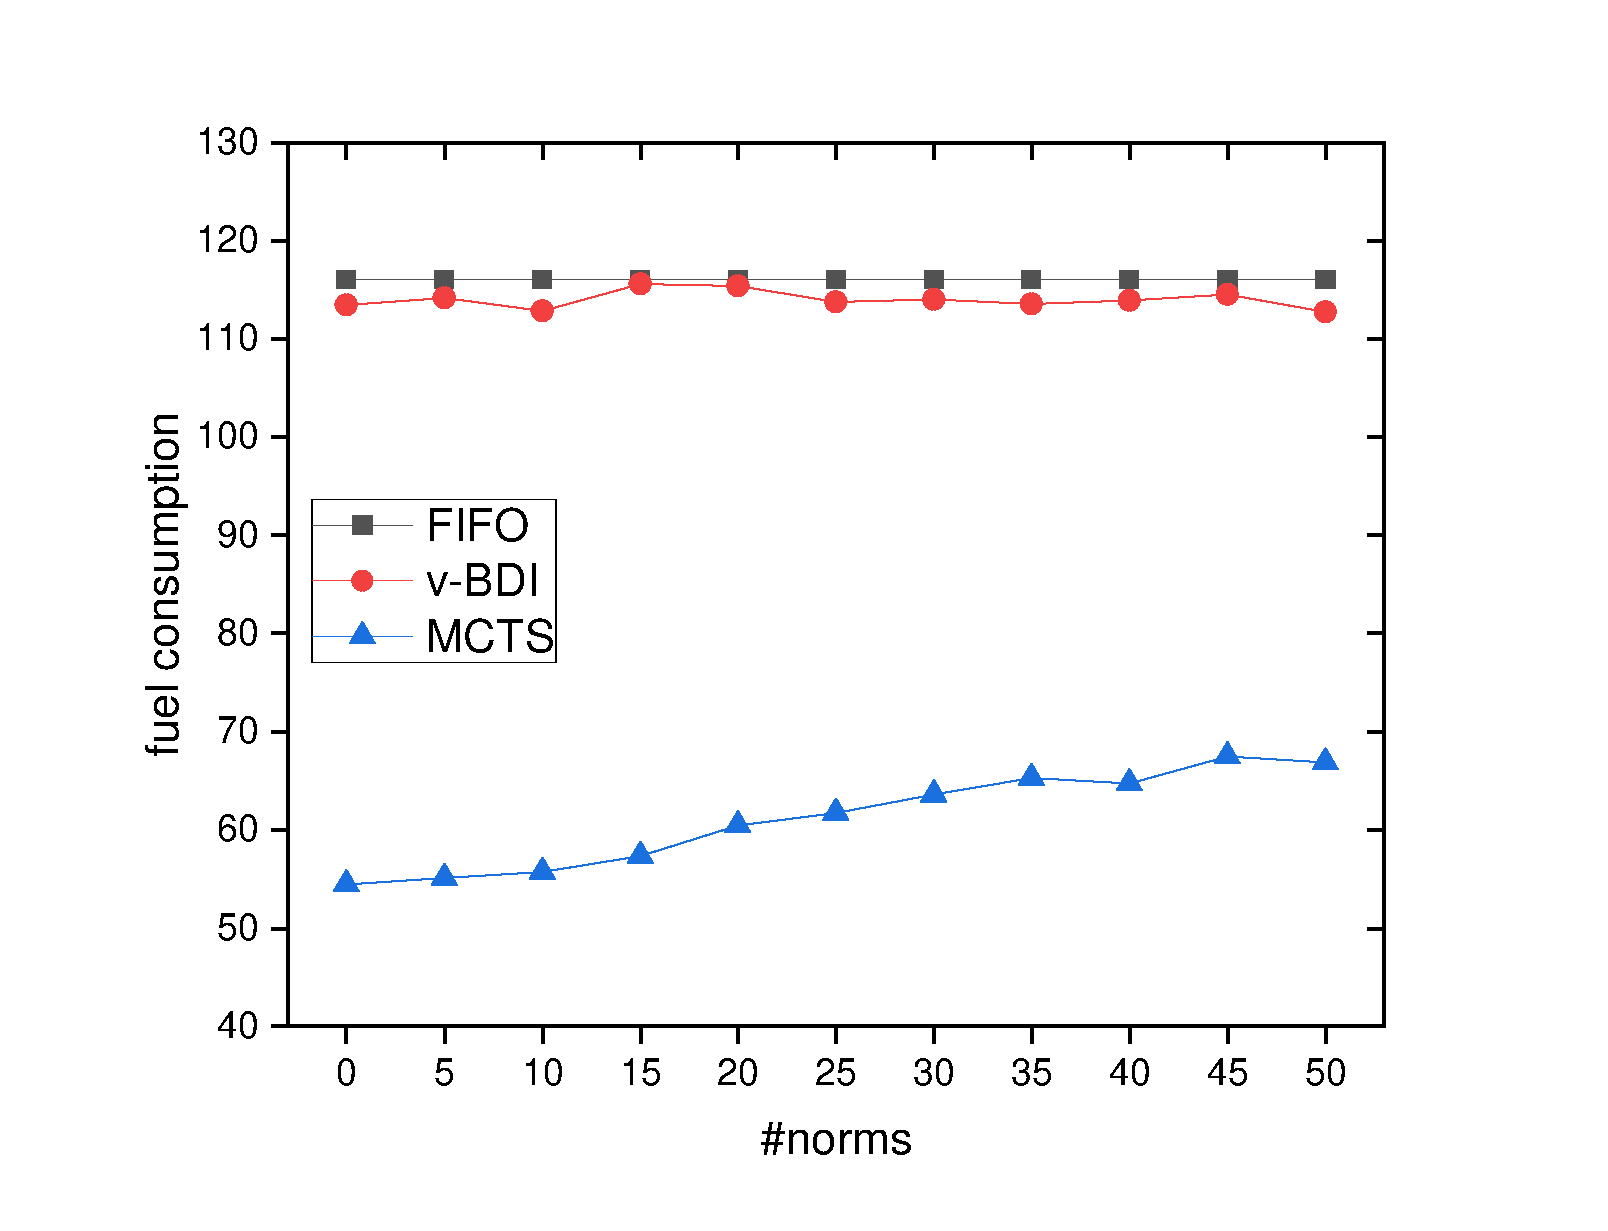
\includegraphics[scale=0.18]{normsX_consumptionY_fixGoals10.pdf}
  \captionsetup{justification=centering}
  \caption{Fuel consumption}
  \label{fig:normsX_consumptionY_fixGoals10}
\end{subfigure}
\begin{subfigure}{.47\textwidth}
  \centering
  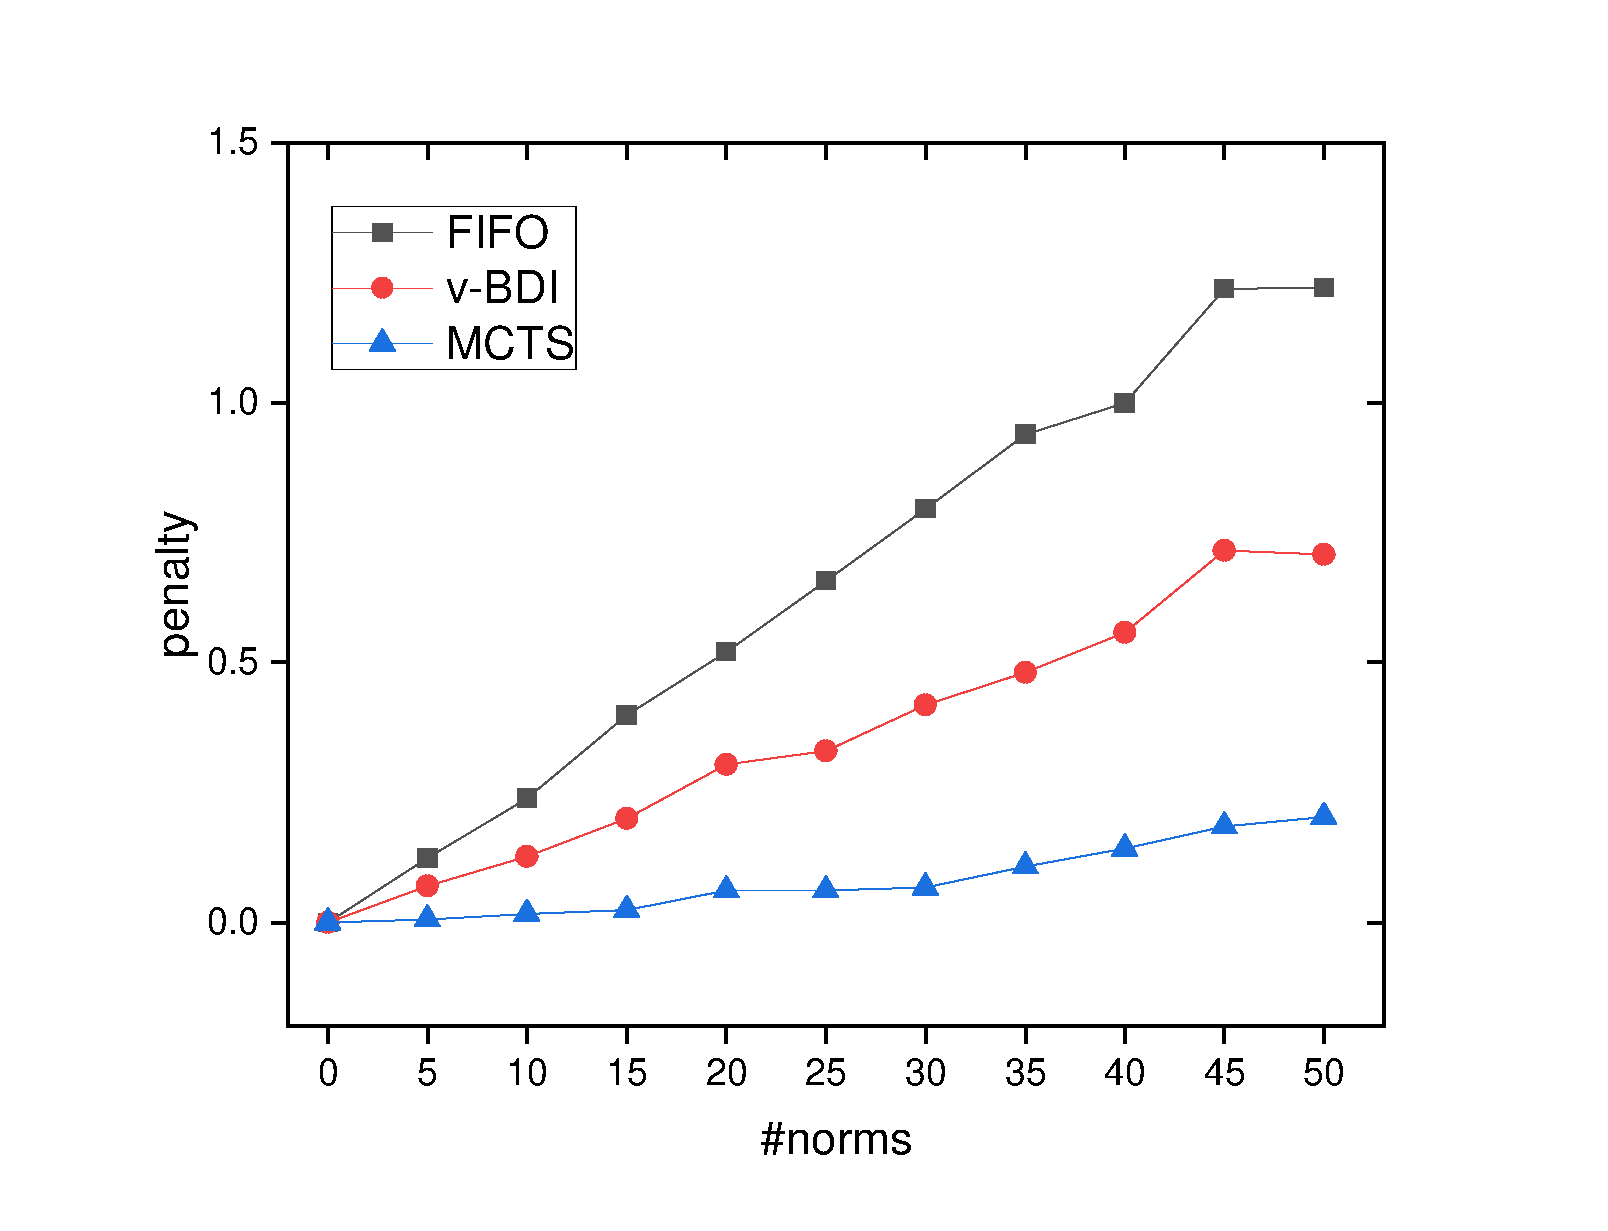
\includegraphics[scale=0.18]{normsX_penaltyY_fixGoals10.pdf}
  \captionsetup{justification=centering}
  \caption{Penalty}
  \label{fig:normsX_penaltyY_fixGoals10}
\end{subfigure}
\captionsetup{justification=centering}
\bicaption{目标数量为10下的实验结果}{Overall utility, fuel consumption and penalty with fixed \#goals 10}
\label{fig:all_fixGoals10}
\end{figure}
% Figure info
图\ref{fig:normsX_valueY_fixGoals10}展示了不同数量norm情况下每个方法的效用价值。正如所预料的,NMG的性能表现最差。
% explanation
有一个特殊情况值得注意的是当norm的数量为0时,NMG与v-BDI没有性能差异。因为当norm数量为0时,智能体是否考虑norm已经无关紧要,性能表现最终取决于实现目标的数量与电池消耗量。MCTS有着最优秀的性能表现。即使在norm的数量为0的情况下,MCTS也比NMG和v-BDI有着更好的性能表现,因为其可以利用到不同意图间的协同效应。
% Details
当norm的数量较多时,MCTS与其他方法的差距更为明显。

% Consumption
图\ref{fig:normsX_consumptionY_fixGoals10} 展示了每种方法在不同norm数量下的平均电量消耗。NMG与v-BDI消耗的电量非常相似,但是由于v-BDI的计划选择机制与NMG不同,导致与NMG相比略有波动。

% MCTS performance
在所有情况下,与NMG和v-BDI相比,MCTS消耗的电量明显更少。然而,随着norm数量的增加,MCTS的电量消耗有所增加。这是因为MCTS既重视电量消耗,也重视norm的影响。随着norm的数量增加,为了使整体收益最大化,MCTS可能会放弃一些可以利用的意图间协同效应以更好地避免违反norm的情况发生。

% Penalty
图\ref{fig:normsX_penaltyY_fixGoals10}展示了不同norm数量下各方法的平均受惩罚值。可以看出,NMG总是受到最多的惩罚值,而MCTS受到的惩罚值则比其他两种方法低很多。当norm数量较大时,不同方法收惩罚值的差异更为明显。当norm的数量为50时,MCTS仅仅受到0.2的惩罚值,而v-BDI几乎是MCTS的3倍,NMG几乎是MCTS的6倍。

\subsection{动态环境实验}
为了探究不同方法在动态环境下的性能表现,以下实验假定并非所有目标都在初始时给定。相反,一些目标会在运行时分配给智能体。
%
本实验使用变量$n$来代表两个目标的分配时间间隔。即每隔$n$周期给智能体分配一个新的目标(假定执行一个动作对应一个周期)。

\paragraph{实验四}
和实验一类似,在该实验中norm的数量被设定为10,实现目标的数量从1改变至15。另外,$n$的值被设定为5,即每隔5个周期给智能体分配一个新的目标。
\begin{figure}
\centering
\begin{subfigure}{.47\textwidth}
  \centering
  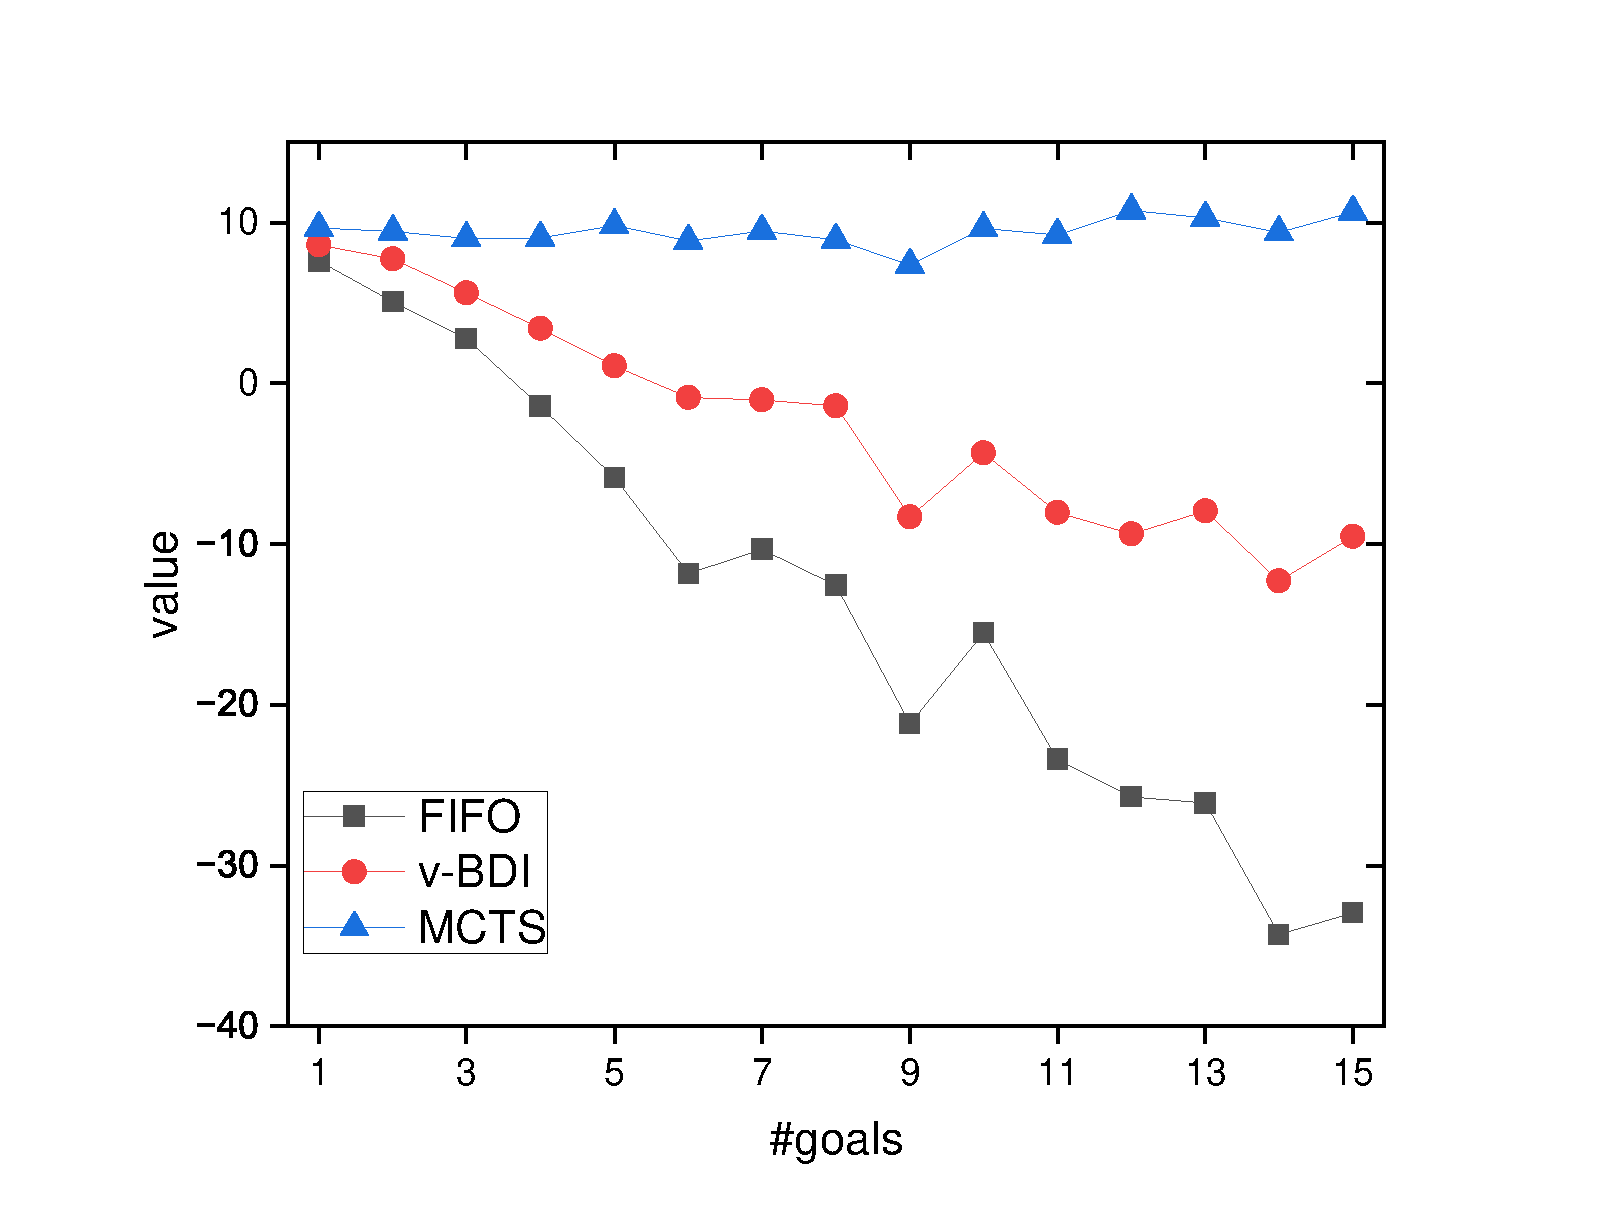
\includegraphics[scale=0.18]{goalsX_valueY_fixNorms10_dynamic.pdf}
  \captionsetup{justification=centering}
  \caption{Utility}
  \label{fig:goalsX_valueY_fixNorms10_dynamic}
\end{subfigure}

\begin{subfigure}{.47\textwidth}
  \centering
  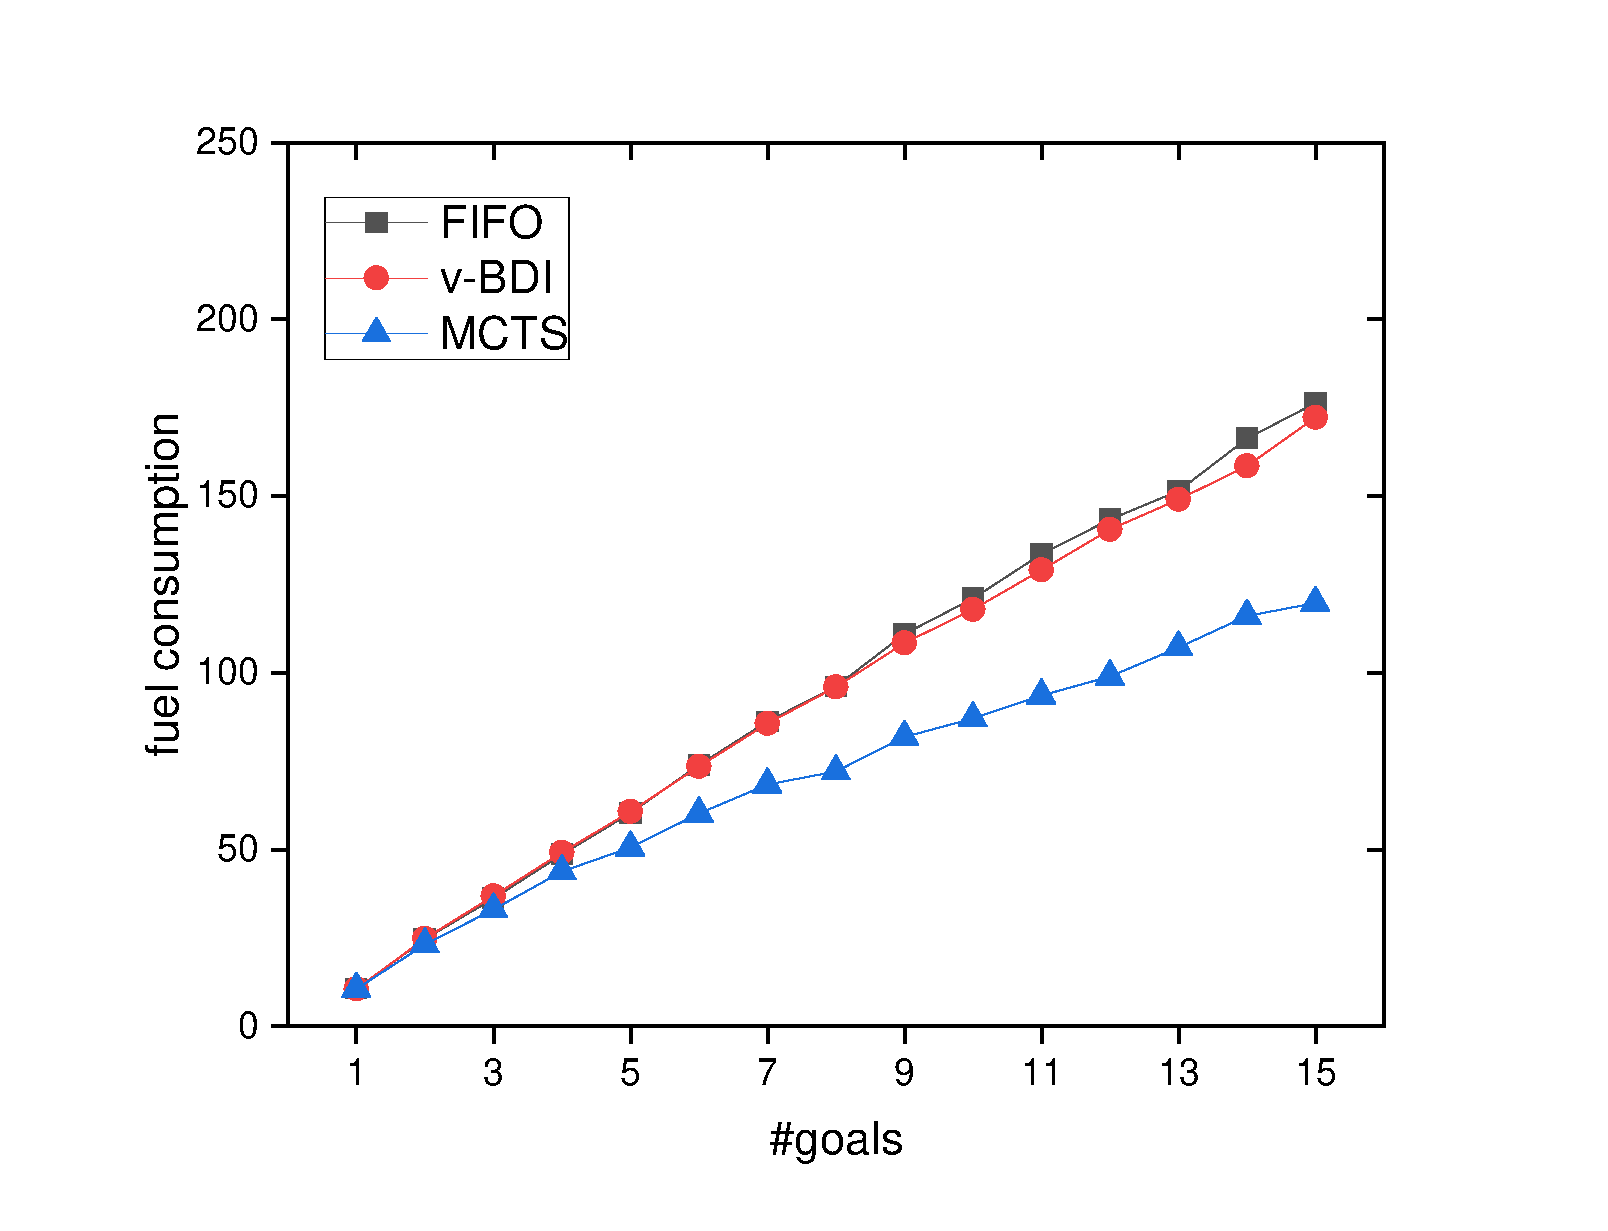
\includegraphics[scale=0.18]{goalsX_consumptionY_fixNorms10_dynamic.pdf}
  \captionsetup{justification=centering}
  \caption{Fuel consumption}
  \label{fig:goalsX_consumptionY_fixNorms10_dynamic}
\end{subfigure}
\begin{subfigure}{.47\textwidth}
  \centering
  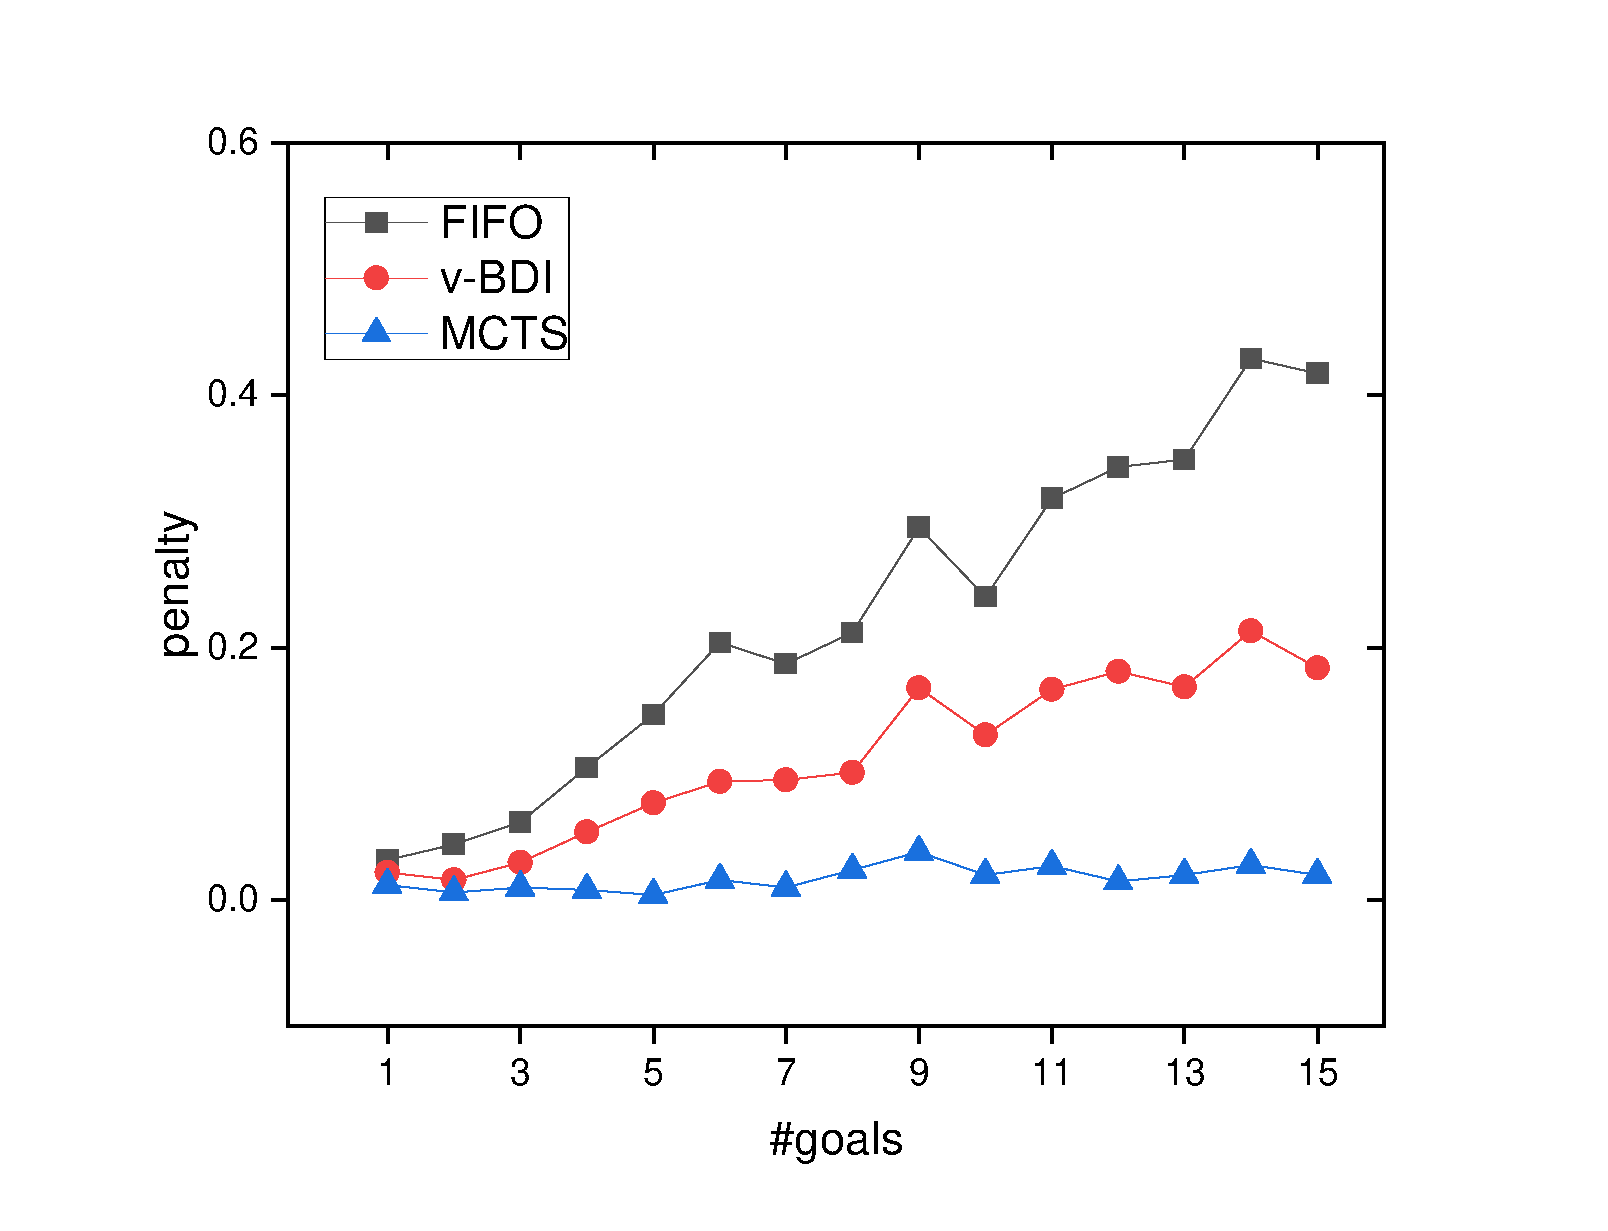
\includegraphics[scale=0.18]{goalsX_penaltyY_fixNorms10_dynamic.pdf}
  \captionsetup{justification=centering}
  \caption{Penalty}
  \label{fig:goalsX_penaltyY_fixNorms10_dynamic}
\end{subfigure}
\captionsetup{justification=centering}
\bicaption{norm数量为10下的实验结果}{Overall utility, fuel consumption and penalty with fixed \#norms 10}
\label{fig:all_fixNorms10_dynamic}
\end{figure}

图\ref{fig:goalsX_valueY_fixNorms10_dynamic}展示了每种方法的总价值。NMG和v-BDI的性能与实验一几乎相同,而MCTS则有较为明显的性能下降。这是因为即使目标在不同时间被分配给智能体,也不会影响NMG和v-BDI实现目标的顺序。唯一的区别在于,如果所有目标都在初始给定,NMG和v-BDI有更多的机会从“意料之外”的协同效应中受益。即当一个目标位于智能体移动到某一个位置的途中时,智能体可以顺便实现途中的目标,从而达到节省执行步骤的效果,这使得电量消耗降低以及违反norm的数量降低。然而,MCTS的方法受到环境动态性的影响,并行执行的目标数量降低,而智能体无法预测未来,只能根据当前状态计算出“最佳”的决策,导致对不同意图间协同效应的利用价值降低。尽管如此,MCTS的表现依然显著优于NMG和v-BDI。

% Consumption
图\ref{fig:goalsX_consumptionY_fixNorms10_dynamic} 展示了各方法的电量消耗。NMG和v-BDI的电量消耗与实验一几乎相同,而MCTS方法由于环境的动态性导致其难以利用协同效应,使得电量消耗有所增加,但是其表现依旧优于NMG和v-BDI。

% penalty
图\ref{fig:goalsX_penaltyY_fixNorms10_dynamic}展示了各方法所受到的惩罚值。与实验一相比,每种方法所受到的惩罚值几乎没有变化(目标数量相同的情况下)。这表明当前设定下的环境动态性不足以早成显著的惩罚值差异。

\vspace{3cm}

\paragraph{实验五}
在实验五中,norm的数量被设定为30。其他实验设定与实验四相同。实验结果如图\ref{fig:all_fixNorms30_dynamic}所示。
\begin{figure}
\centering
\begin{subfigure}{.47\textwidth}
  \centering
  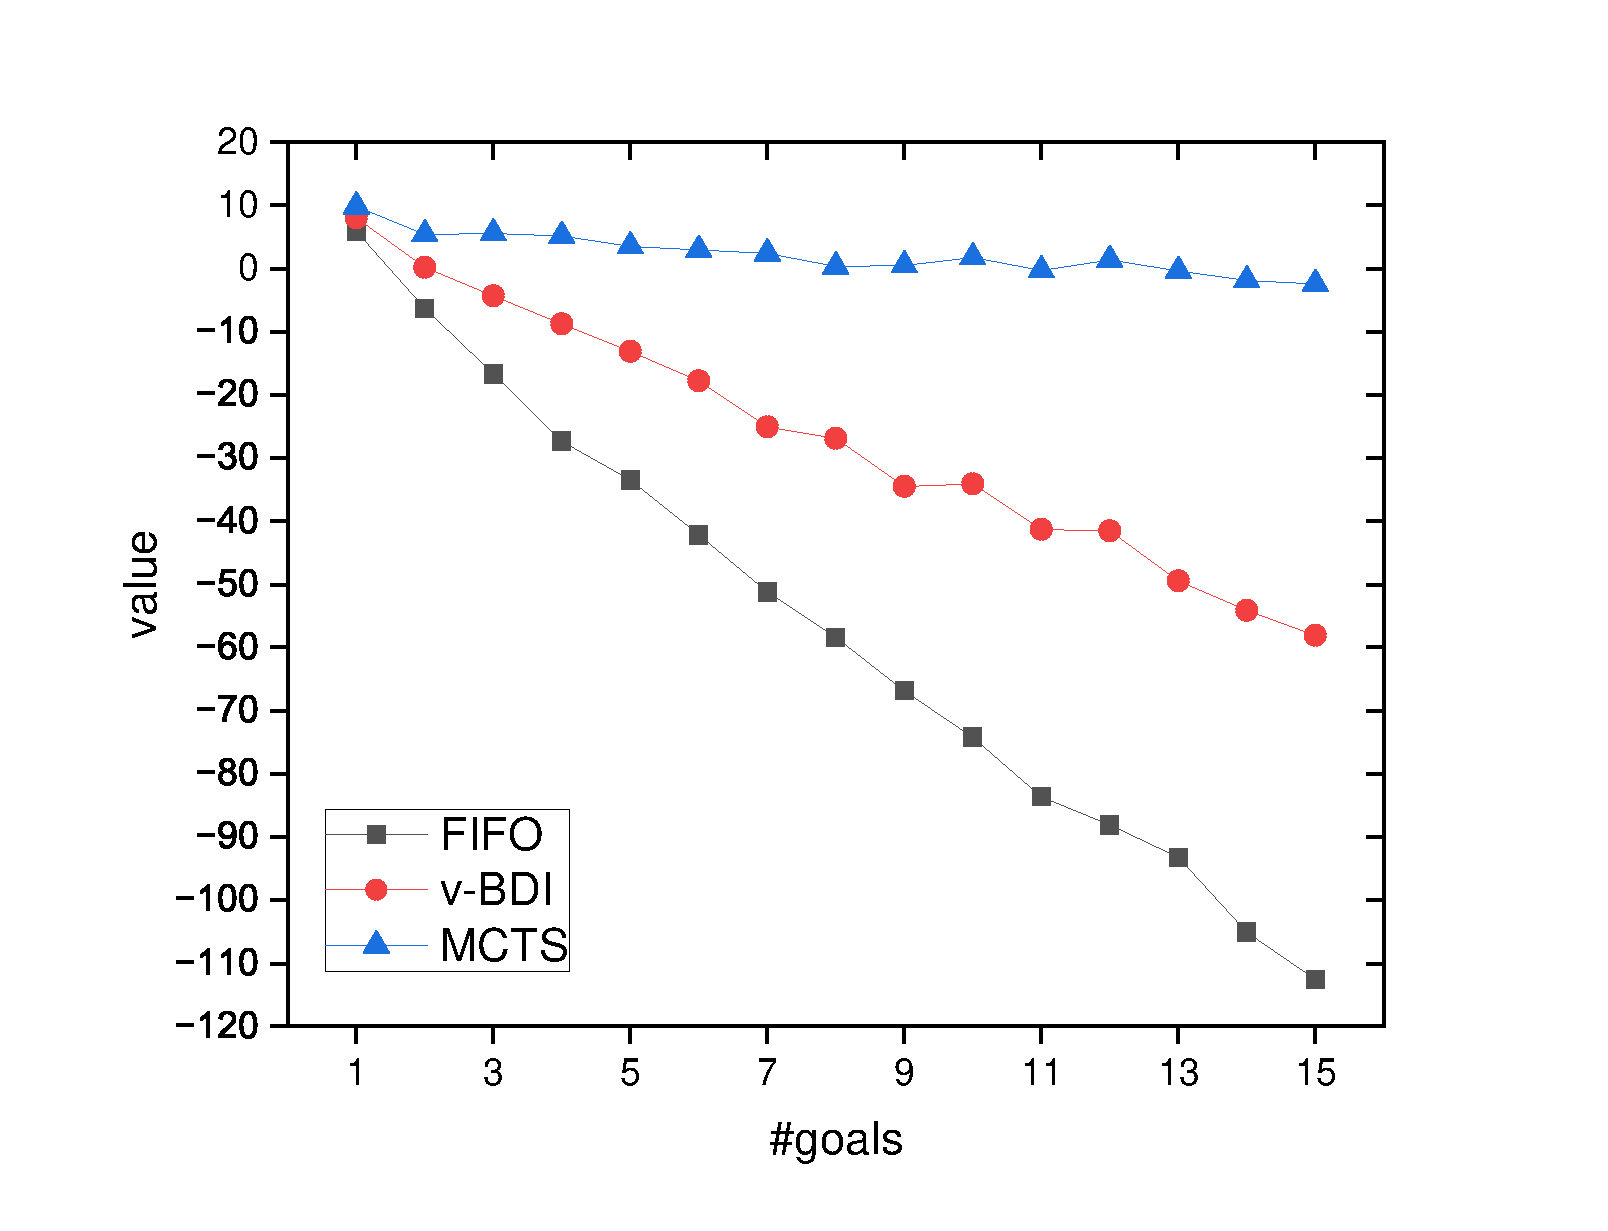
\includegraphics[scale=0.18]{goalsX_valueY_fixNorms30_dynamic.pdf}
  \captionsetup{justification=centering}
  \caption{Utility}
  \label{fig:goalsX_valueY_fixNorms30_dynamic}
\end{subfigure}

\begin{subfigure}{.47\textwidth}
  \centering
  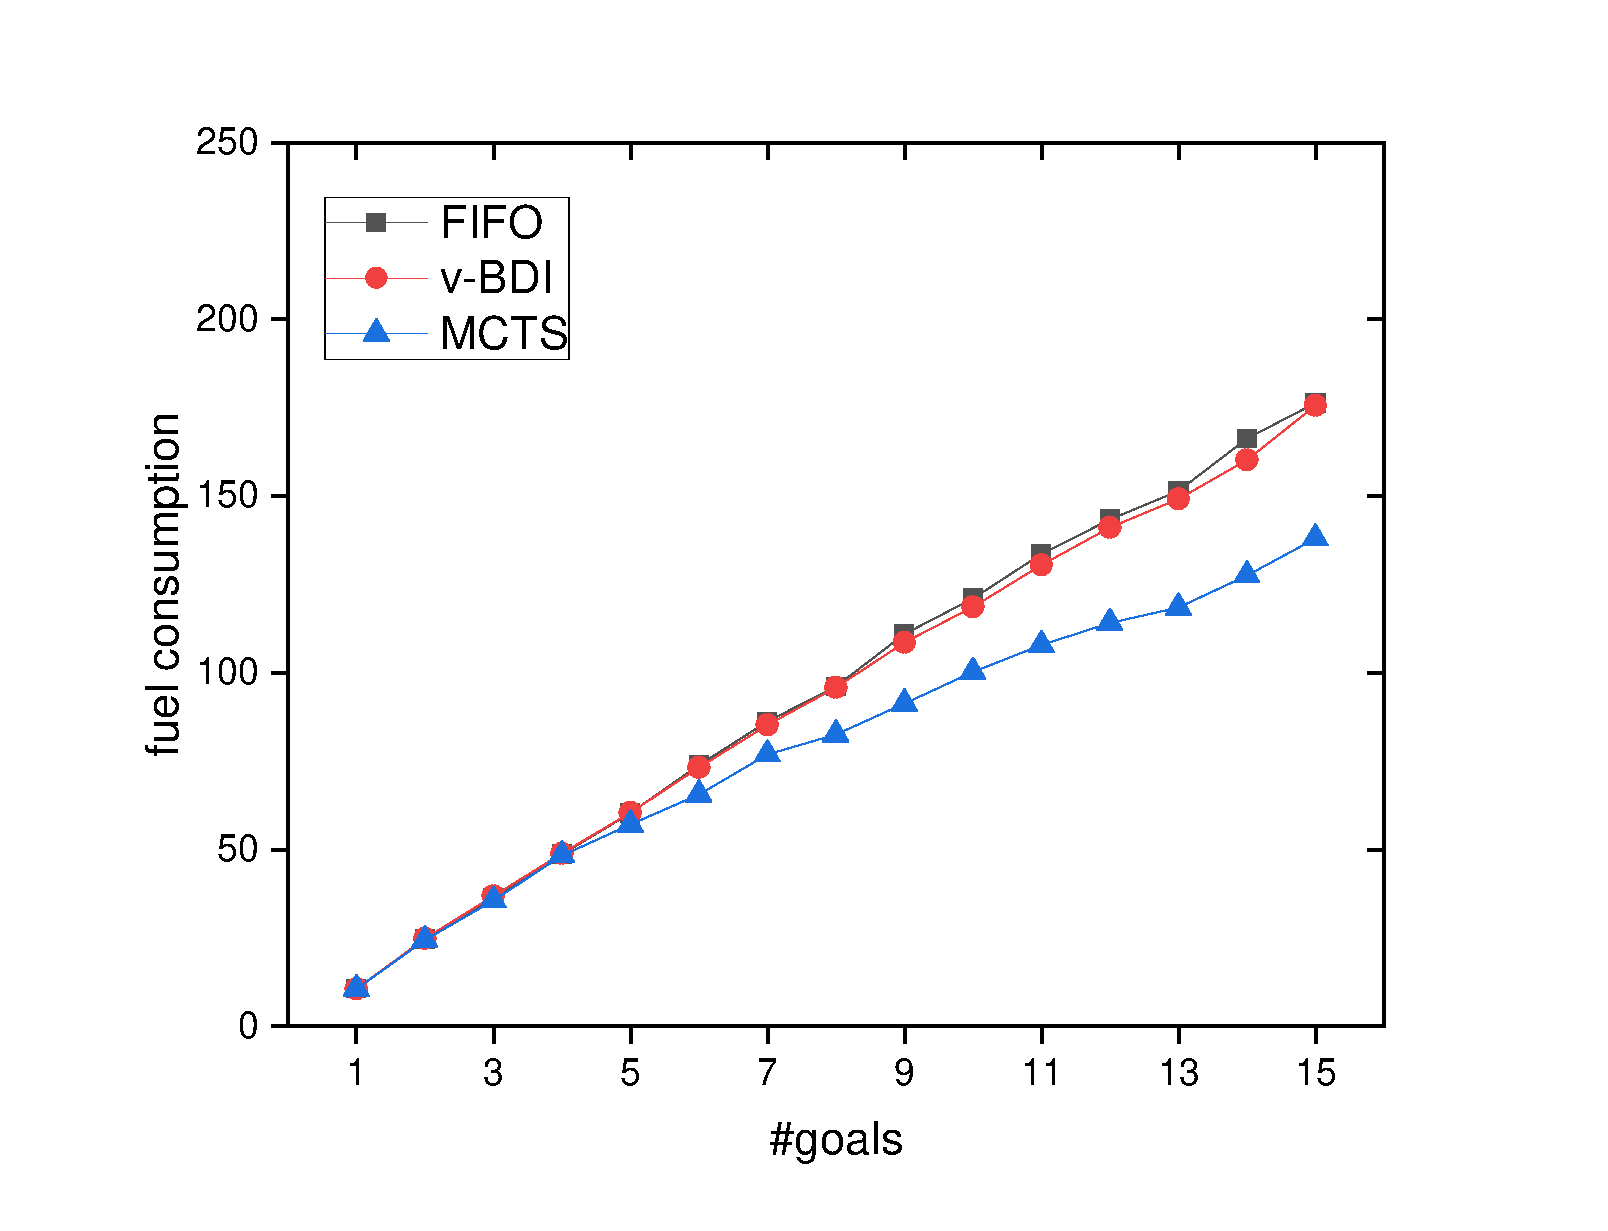
\includegraphics[scale=0.18]{goalsX_consumptionY_fixNorms30_dynamic.pdf}
  \captionsetup{justification=centering}
  \caption{Fuel consumption}
  \label{fig:goalsX_consumptionY_fixNorms30_dynamic}
\end{subfigure}
\begin{subfigure}{.47\textwidth}
  \centering
  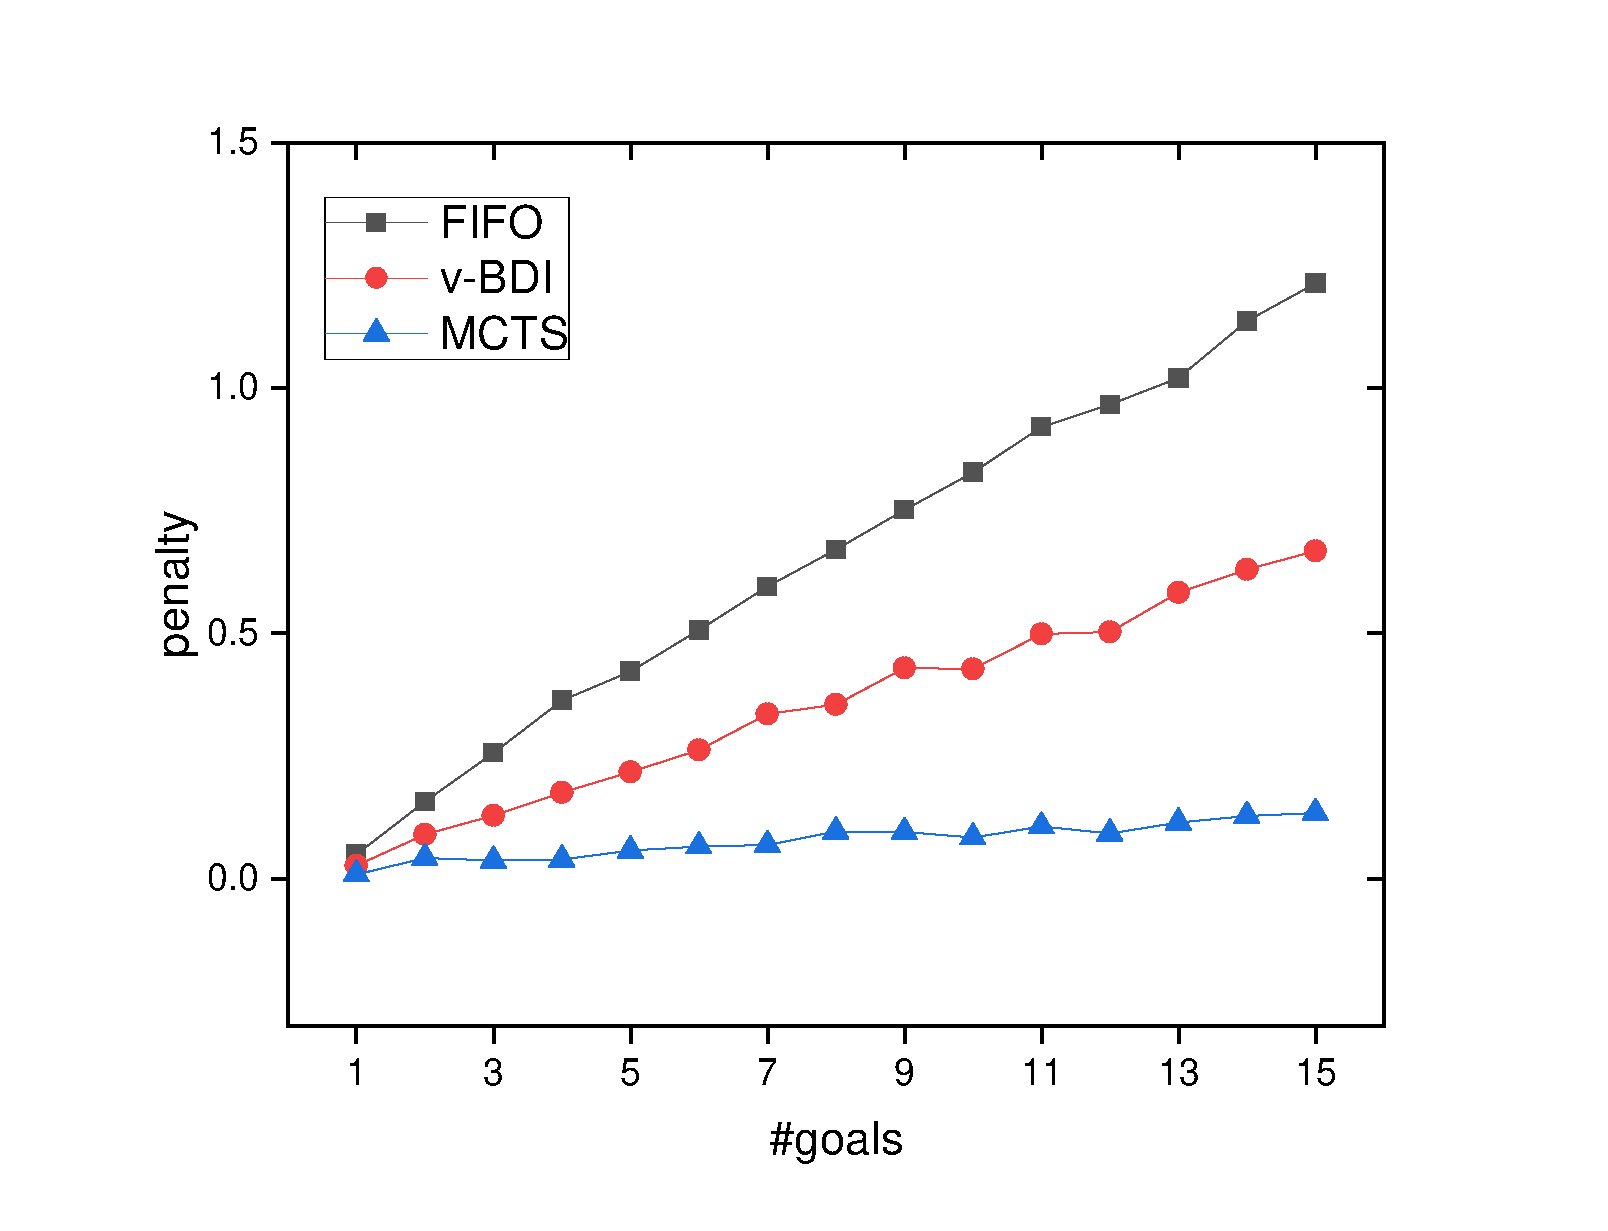
\includegraphics[scale=0.18]{goalsX_penaltyY_fixNorms30_dynamic.pdf}
  \captionsetup{justification=centering}
  \caption{Penalty}
  \label{fig:goalsX_penaltyY_fixNorms30_dynamic}
\end{subfigure}
\captionsetup{justification=centering}
\bicaption{norm数量为30下的实验结果}{Overall utility, fuel consumption and penalty with fixed \#norms 30}
\label{fig:all_fixNorms30_dynamic}
\end{figure}

该设定下的实验结果与实验二非常类似。相比于NMG和v-BDI,MCTS有着显著的性能优势。v-BDI比NMG的性能表现更好,但是仍然无法与MCTS相比较。特别是当实现目标数量较大时,MCTS的性能优势尤为明显。

\paragraph{实验六}
在实验六中,智能体实现目标的数量被固定为10,norm的数量被固定为30。分配目标的时间间隔$n$从1改变至15。具体实验结果如图\ref{fig:all_fixGoals10Norms30}所示。

\begin{figure}
\centering
\begin{subfigure}{.47\textwidth}
\centering
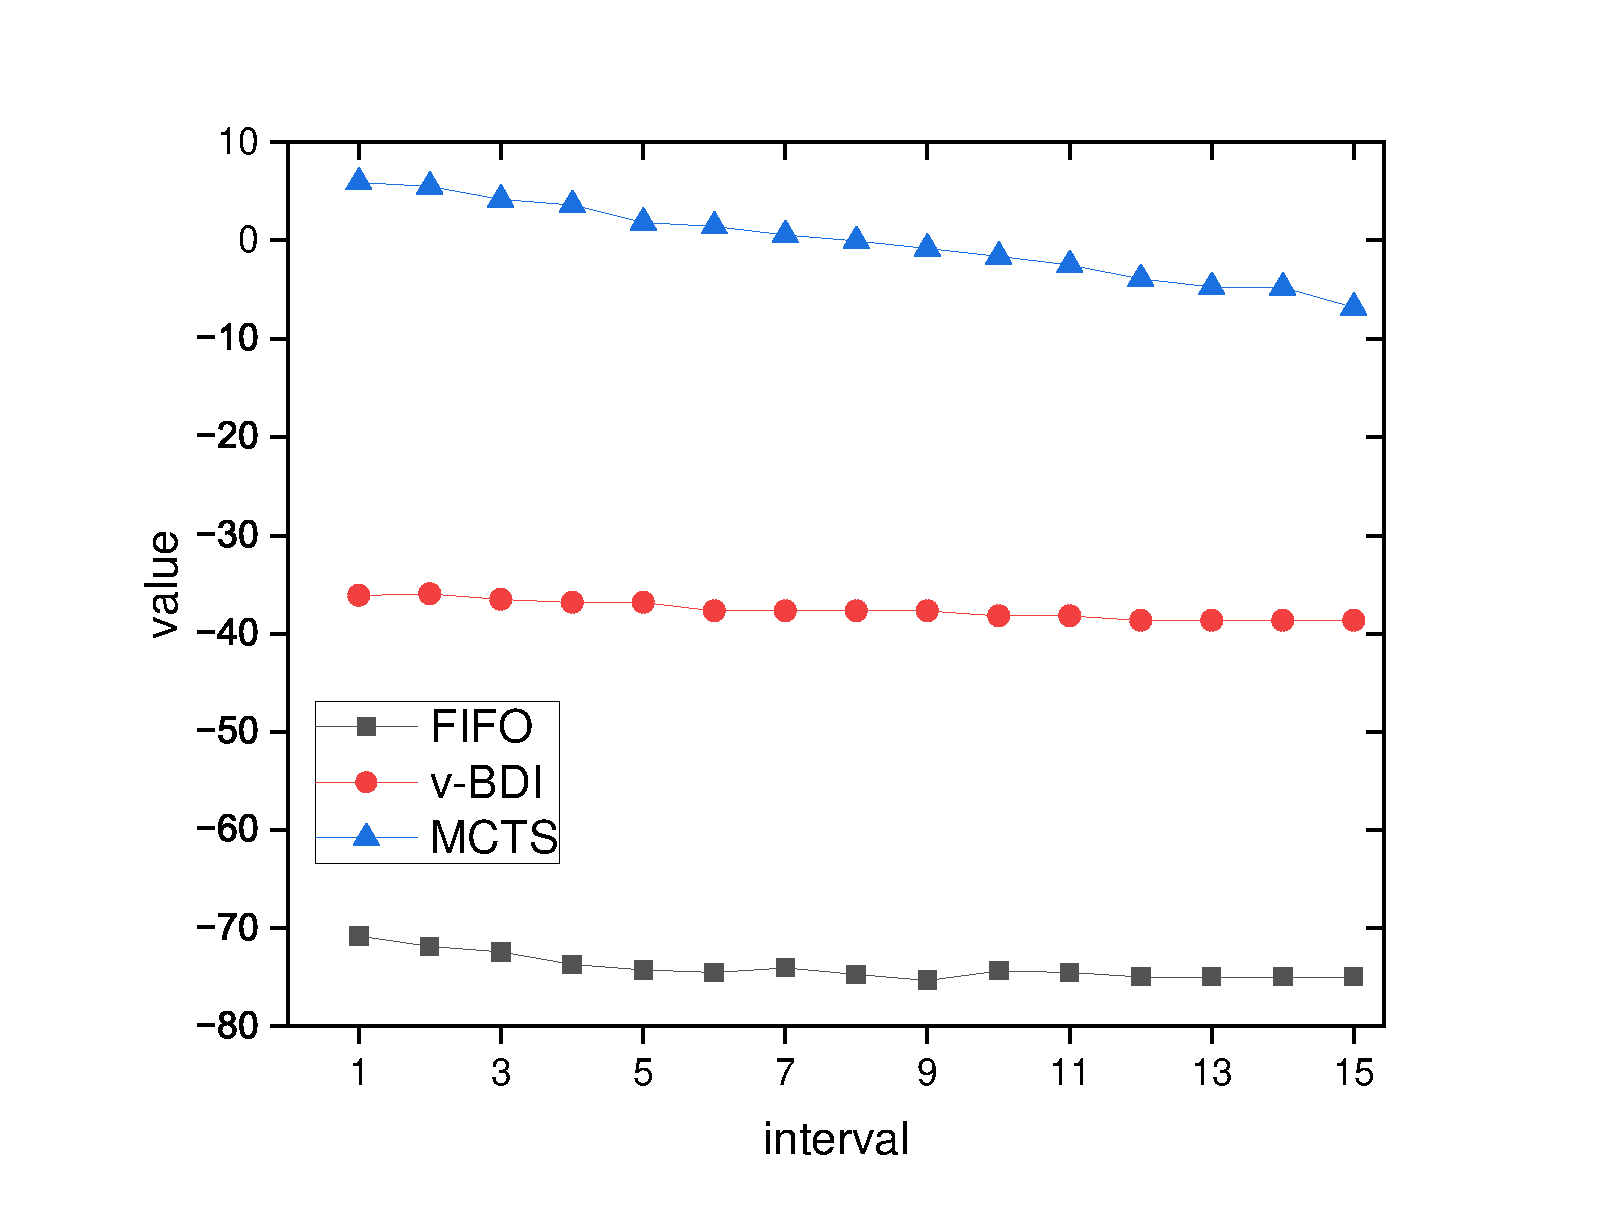
\includegraphics[scale=0.18]{intervalX_valueY_fixGoals10.pdf}
\captionsetup{justification=centering}
\caption{Overall utility}
\label{fig:intervalX_valueY_fixGoals10}
\end{subfigure}

\begin{subfigure}{.47\textwidth}
  \centering
  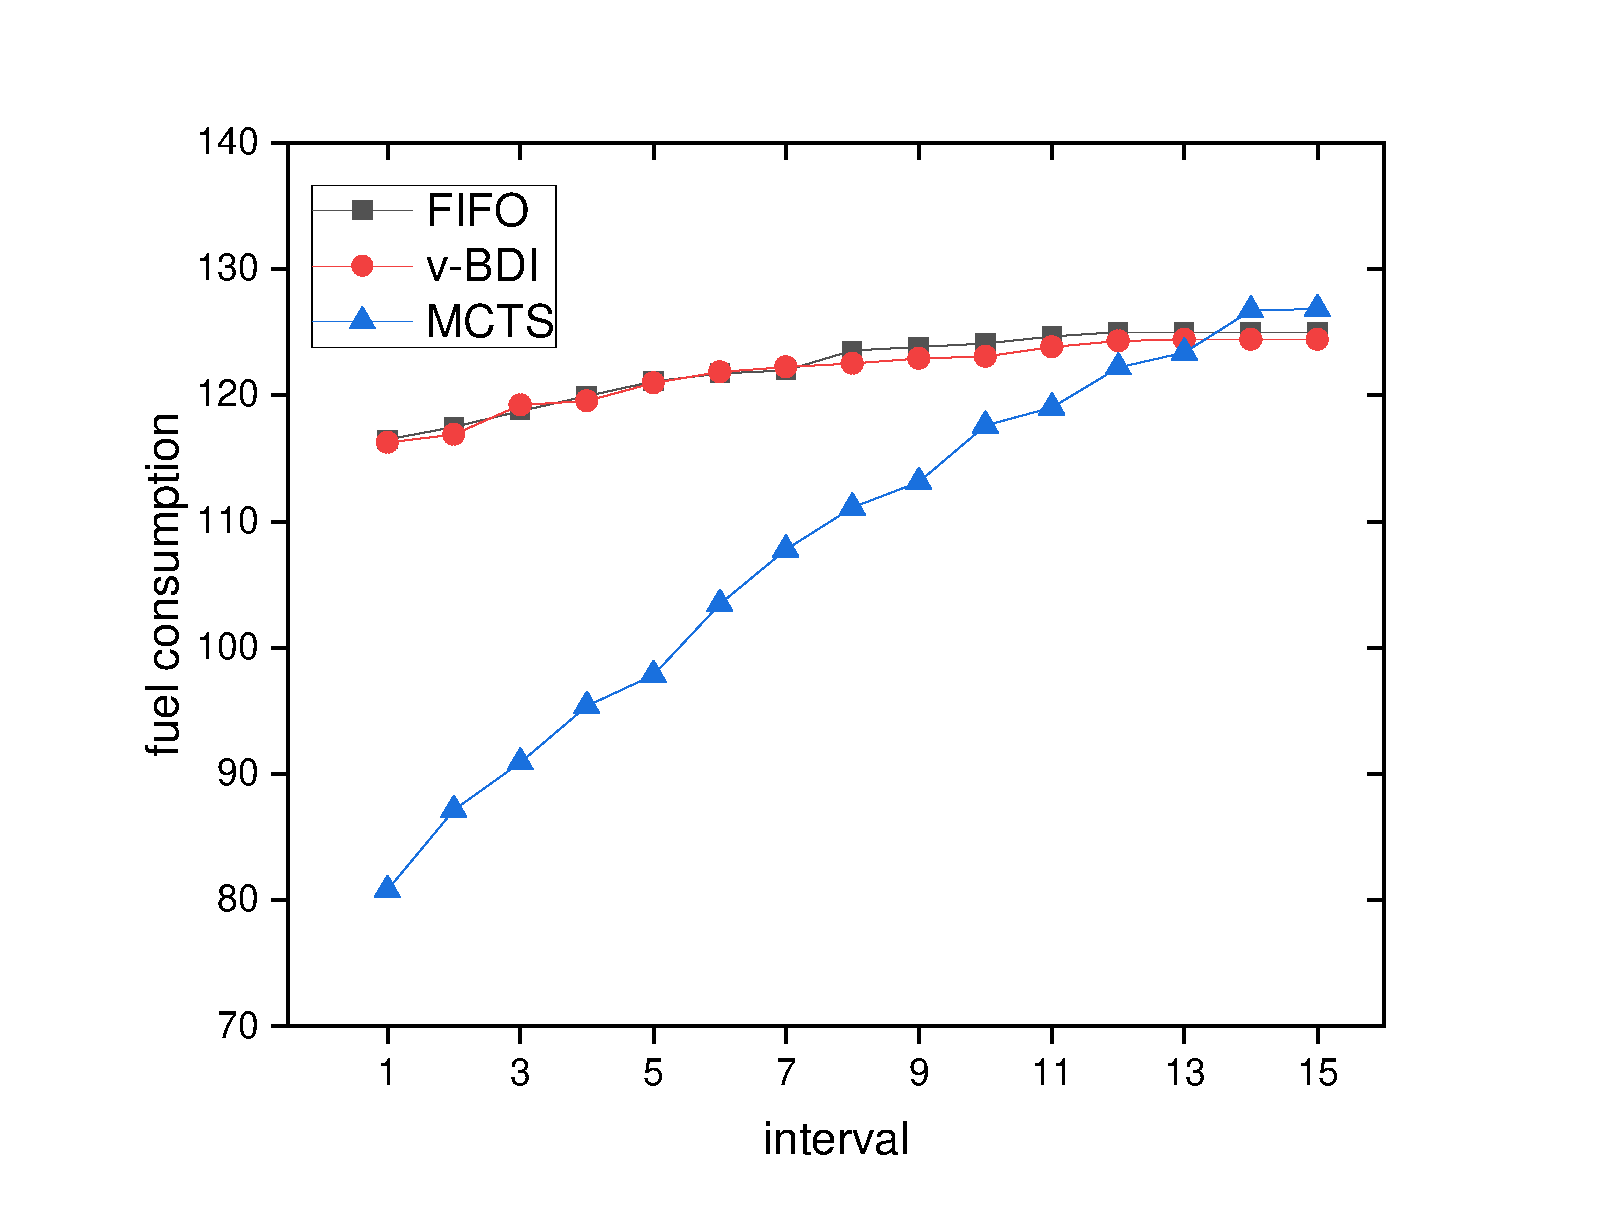
\includegraphics[scale=0.18]{intervalX_consumptionY_fixGoals10.pdf}
  \captionsetup{justification=centering}
  \caption{Fuel consumption}
  \label{fig:intervalX_consumptionY_fixGoals10}
\end{subfigure}
\begin{subfigure}{.47\textwidth}
  \centering
  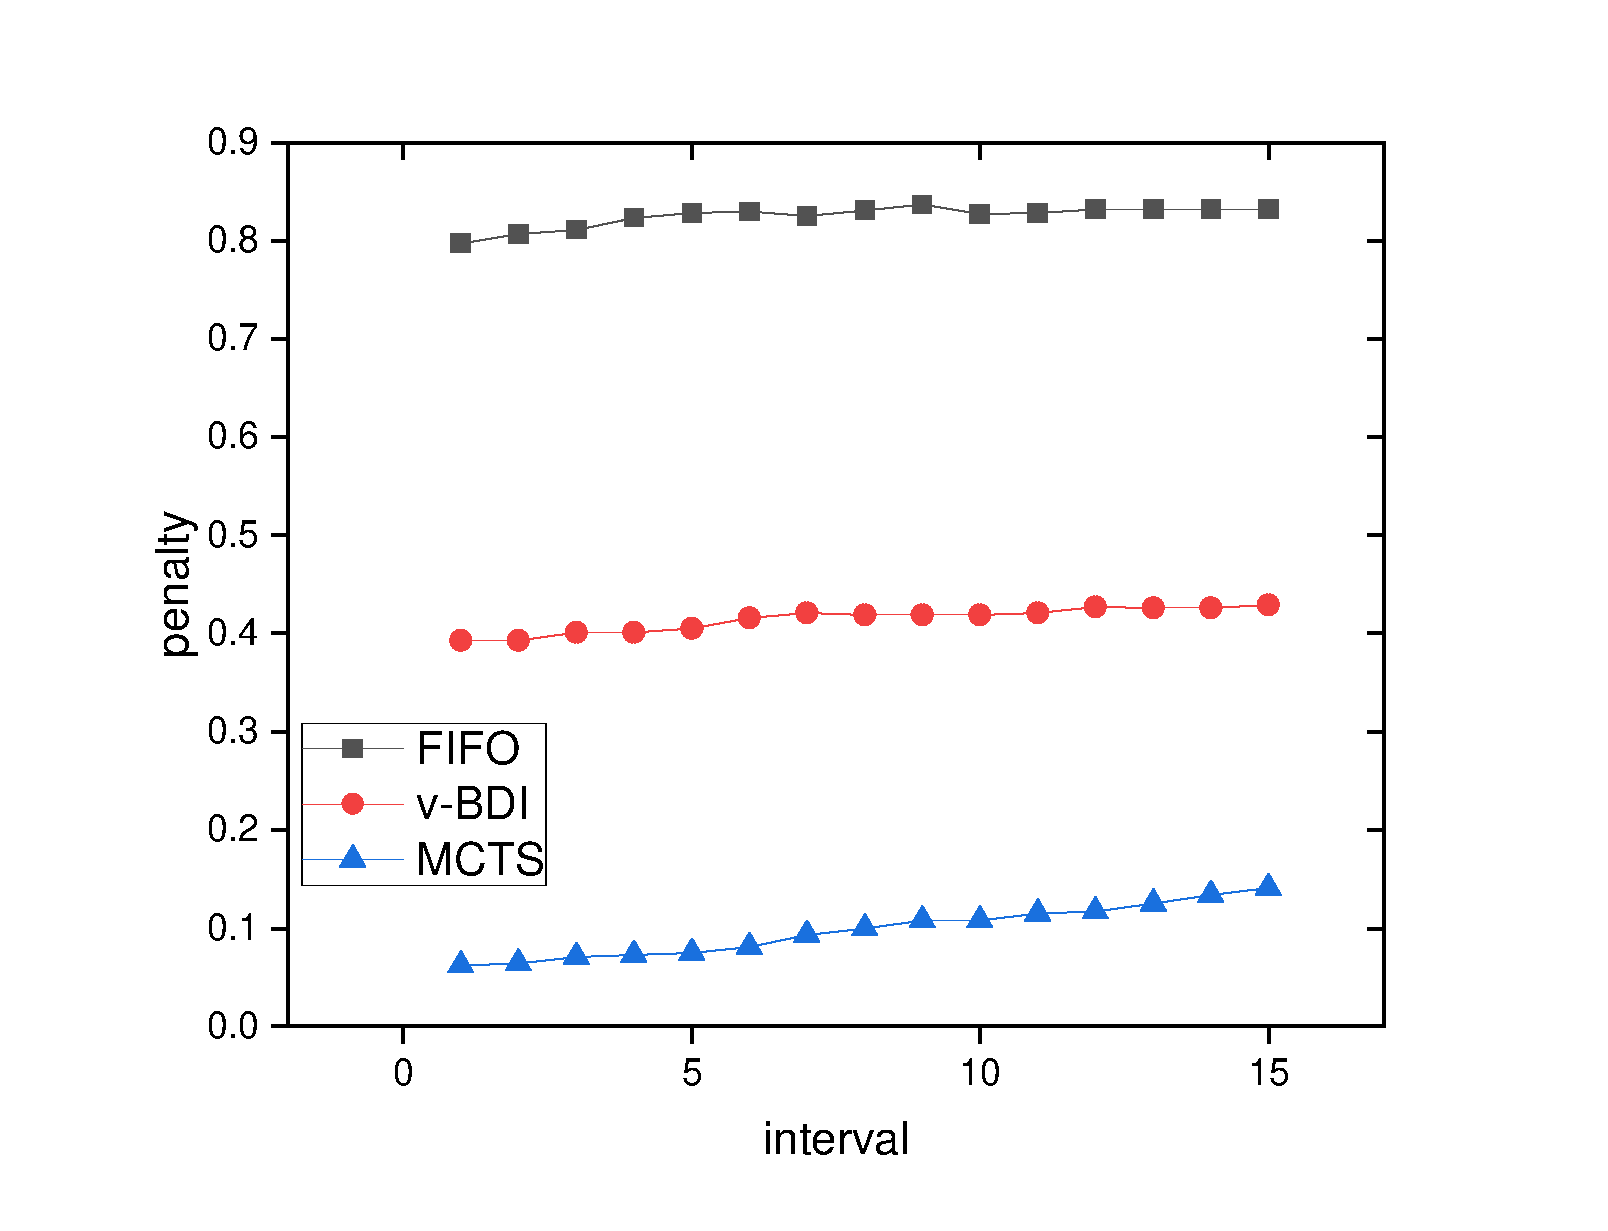
\includegraphics[scale=0.18]{intervalX_penaltyY_fixGoals10.pdf}
  \captionsetup{justification=centering}
  \caption{Penalty}
  \label{fig:intervalX_penaltyY_fixGoals10}
\end{subfigure}
\captionsetup{justification=centering}
\bicaption{目标数量为10且norm数量为30下的实验结果}{Overall utility, fuel consumption and penalty with fixed \#goals 10 and \#norms 30}
\label{fig:all_fixGoals10Norms30}
\end{figure}
% Figure information
如图\ref{fig:intervalX_valueY_fixGoals10}所示,MCTS方法依旧优于NMG和v-BDI。然而,MCTS方法的收益随着时间间隔的增加而有所减少。
% Reason
当$n$较小时,有更多的并行目标,因此智能体可以更多地利用多意图间的协同效应。当$n$设定为15时,智能体几乎无法从协同效应中受益,因为这种情况下大多数时候智能体只有一个目标。然而,MCTS仍然比v-BDI表现更为优秀,因为MCTS可以更好地对norm进行决策推理并利用多意图间协同效应,从而减少移动量以及违反norm的次数。

% Consumption
图\ref{fig:intervalX_consumptionY_fixGoals10}展示了不同时间间隔下各方法的平均耗电量。所有方法的耗电量都随着时间间隔的变大而增加。然而,值得注意的是,与NMG和v-BDI相比,MCTS的电量消耗增长更为明显。当$n$大于13时,其电量消耗甚至大于NMG和v-BDI。
% Explanation
这是因为MCTS主要考虑的是整体效用值,这导致其放弃了一些原本可以利用的意图间协同效应而避免违反norm,已获得更高的整体收益。
% penalty
图\ref{fig:intervalX_penaltyY_fixGoals10}展示了每种方法在不同时间间隔下单平均惩罚值。与NMG相比,v-BDI收到的惩罚值更少。由于固定的实现目标顺序,这两种方法的惩罚值几乎不会随着时间间隔的增加而改变。然而,相比之下MCTS所受惩罚值非常低。另外,由于NCMTS总是基于当前环境进行决策,导致随着$n$的增加,MCTS所执行步骤数量增加,最终使得智能体违反更多的norm,受到的惩罚值有明显的增加。
\section{本章总结}
本章提出了一种基于\SA 的意图调度算法\SAN 。\SAN 可以在norm约束下对智能体进行意图调度。另外,基于火星探测器的模拟场景,本章在静态环境以及动态环境下对\SAN 的性能进行了分析。实验结果表明\SAN 与其他方法(NMG和v-BDI)相比有着显著的性能优势。即使在norm的数量非常多时,\SAN 仍然可以可靠地地避免对norm
的违反同时高效利用多个并发意图之间的协同效应,最终得到较高的整体价值收益。

本文的下一章将考虑如何基于时序逻辑(Linear Temporal Logic,LTL),并将其与MCTS算法有效结合,使得智能体同时处理实现型目标、维持型目标以及norm;并且提高智能体的可扩展性,允许智能体处理各种类型的用LTL表示的目标和norm。

\chapter{基于LTL的表示与决策方法}\label{ltl}
本章提出一种基于LTL的智能体目标和norm的表示方法,并将其与\SA 算法结合,提出一种同时支持实现型目标、维持型目标以及norm的意图调度算法\SAT。本章实验部分对\SAT 的性能表现在不同的资源储备量下进行了分析,并与Duff等人提出的PMG\cite{DBLP:conf/atal/DuffHT06}算法和Meneguzzi等人提出的v-BDI算法\cite{DBLP:journals/eaai/MeneguzziROVL15}进行了比较,实验结果表明\SAT 的性能表现相对PMG和v-BDI有显著优势\footnote{在前两章中,本文分别将\SAM 与PMG进行对比,将\SAN 与v-BDI进行对比。}。
\section{多类型的目标与norm}
在许多社会仿真场景中,目标可能有丰富的类型,例如需要智能体在一段时间内保持某一特定状态的维持型目标,或是在某些特定情况下,只有在满足某些特定条件时才最求的条件目标。此外,智能体的行为可能受到norm的约束,智能体需要在决策时加入对norm的考虑,以避免违反norm,或者选择性地违反norm以实现更重要的目标。本文第\ref{mg}章研究了了如何同时对实现型目标和维持型目标进行意图调度,并提出了\SAM 算法;第\ref{norm}章研究了了如何在norm约束下进行意图调度,并提出了\SAN 算法。本章考虑更为实际的社会仿真模拟场景:在本章中,各种类型的目标与norm统一以线性时序逻辑(Linear Temporal Logic, LTL)的形式表示,而智能体需要对LTL表示的目标或norm进行意图调度。

Dastani等人\cite{DBLP:conf/atal/DastaniRW11}提出了一种基于LTL表示各种类型目标(如实现型目标、维持型目标、行动目标等)的框架。在其框架中一个维持型目标被表示为$\alpha \cup \tau$,其中$\alpha$为智能体需要维持的条件,$\cup$表示“直到”,而$\tau$表示终止条件。因此$\alpha \cup \tau$表示维持$\alpha$,直到$\tau$被满足。LTL的表示能力是通用且强大的,足以表示各种类型的目标并拓展现有目标类型。为了实现这些LTL形式的目标Dastani等人也在其研究中提出一种转换方法,能够将LTL公式转变为一般智能体编程语言所支持的普通实现型目标和维持型目标。其LTL目标的转化规则以条件-动作对(Condition-Action Pairs)来表示。其描述了在某个特定环境状态下的目标状态转变(由LTL目标转化为基本目标)。Dastani等人\cite{DBLP:conf/atal/DastaniRW11}描述了两种类型的条件-动作对:通用性的以及领域专用的条件-动作对。通用性的条件动作对适用于该框架给定的目标形式,而领域专用的条件-动作对则是为特定领域设计的针对特殊表示形式目标的转换方法,目的是提升智能体的适用范围。然而,该框架并没有提供一个一般性的意图调度算法,某些特殊形式的目标仍然需要用户自定义条件-动作对,虽然有一点的拓展性,但加重了用户的负担;此外,该框架也没有考虑到社会仿真场景下的norm,这导致其不适用于norm约束场景。

Gutierrez等人\cite{DBLP:conf/time/0001KPW22}提出了用于向智能体发出指令的语义模型。该研究以LTL公式的形式表示指令,而智能体则必须以确保LTL公式得到满足的方式行动。此外,该研究假定智能体有一定的后台安全需求(同样以LTL形式表示)需要智能体保护(类似于维持型目标)。该研究对LTL满足(如何行动以满足LTL)与LTL生成(如何根据需求生成LTL)的时间与空间复杂度进行了细致分析。然而,正如其作者所提到,将该语义模型应用于实际的好处仍然未知,因为其并没有被实际应用,无相关实验分析,而仅为一种可能有价值的理论。

Krzisch等人\cite{Krzisch2016}基于经典的规划问题对norm系统进行建模。其考虑了两种norm形式化的方法:一种是仅仅考虑某些场景下的动作(允许或是禁止执行某些动作);另一种则是LTL约束下的一系列状态转移。该研究提出了相应算法以应对norm的约束,然而其算法并没有考虑到多种类型的目标,并且也忽略了多个并发意图下的意图进展问题。

Paxton等人\cite{DBLP:journals/corr/PaxtonRHK17}提出了一种基于深度强化学习的方法以解决复杂动态环境中的规划问题。而该问题被规范表示为一组LTL公式。该方法将MCTS与基于LTL规范训练的人工神经网络结合。该研究在一个仿真自动驾驶场景对人工神经网络的学习能力进行了评估。然而,其在模拟场景下的学习效果并不如预期,并且智能体偶尔会出现奇怪行为。另外,该研究的重点也与对智能体目标、norm的表示关联不大。


\section{使用LTL表示目标与norm}
使用LTL表示目标和norm的优势在于智能体可以在更高的抽象层次处理目标和norm的特性,并且更意图拓展目标和norm的类型。LTL是一种模态时序逻辑方式方式。其由一组有限的命题变量、逻辑运算符(如$\lnot, \lor$)以及时间运算符组成。本文考虑以下时间运算符:
\begin{itemize}
    \item $\square$ 表示是“一直”
    \item $\diamond$ 表示“最终”
    \item and $U$ 表示是“直到”
\end{itemize}
由于在本章中目标和norm基于LTL表示,而LTL编码了状态随时间变化的轨迹,所以本节内容首先对环境及其状态转换进行定义。在此基础上,再给出基于实现型目标、维持型目标以及norm的LTL表达形式(这些目标和norm的表示只是实例,正如\cite{DBLP:conf/atal/DastaniRW11},LTL支持其他更加丰富的目标和norm类型)。

\subsection{环境及其状态转移的表示}
Gutierrez等人\cite{DBLP:conf/time/0001KPW22}描述了一种表示环境及其状态变化的方法。本文基于其方法,对环境以如下方式表示。

本文假设智能体在一个特定的环境中执行,该环境可以处于包含所有可能环境状态集合中的任意一个状态。每个状态都由一组环境变量$V$的确定赋值决定。智能体有一动作集合$\mathcal{A}$,$\mathcal{A}$中的动作可在其前置条件满足时被执行。环境状态从$s_0$开始执行,在一个状态下执行某个动作的结果是将当前环境状态$s$转化为下一个环境状态$s^\prime$。该转变规则由一个转变函数所决定:$\mathcal{T} (s, a) = s^\prime$(为了简单起见,本文假设转变函数为确定型)。在此,本文仅考虑环境状态及其转变,智能体本身的内部状态(如信念、意图等)不在考虑范围内;对于智能体而言,仅仅考虑到能够直接影响到环境状态改变的动作。

形式上,环境由一五元组$E=<\mathcal{S}, V, \mathcal{A},\mathcal{T}, s_0>$所表示,其中:
\begin{itemize}
    \item $\mathcal{S}$为包含所有可能环境状态的非空有限状态集合。
    \item $V$为表示所有环境变量的非空有限集合。
    \item $\mathcal{A}$为智能体可执行的动作集合。
    \item $\mathcal{T}: \mathcal{S} \times \mathcal{A} \rightarrow 2^{\mathcal{S}}$为状态转变函数。
    \item $s_0 \in \mathcal{S}$表示初始环境状态。
\end{itemize}
智能体遵循其运行策略执行动作,直到没有可执行的操作或所有目标都被实现。基于此通识,智能体在环境中执行动作的过程会产生出环境状态与动作的交错序列,该序列被称为\emph{游程}:
\begin{equation}
\rho=s_0 \xrightarrow{\text{$a_0$}} s_1 \xrightarrow{\text{$a_1$}} s_2 \xrightarrow{\text{$a_2$}} \cdots \xrightarrow{\text{$a_{n-1}$}} s_n
\end{equation}
其中$\rho$表示一次游程,本文使用$si(\rho, u)$来索引第$u$个状态,使用$ai(\rho, u)$来索引$\rho$中的第$u$个动作(其中$u$为一个自然数)。本文假设一个游程是有限的,即有一个表示$\rho$结束的最终状态$s_n$。

\subsection{目标、norm的表示}
本文第\ref{mg}章对实现型目标和维持型目标进行了定义,第\ref{norm}章对norm进行了定义,然而并没有对其形式进行统一。
本节正式基于LTL对实现型目标、维持型目标以及norm进行定义。通过这样做,在考虑新的形式的目标和norm时,可以免去对智能体程序的大量修改。智能体仅需要处理新添加的LTL公式即可。此外,这更加便于开发处理丰富类型目标和norm的意图调度算法。

\paragraph{实现型目标}
实现型目标表示了智能体想要达到的环境状态,实现型目标的定义如下:
$$<G_a, C_g, Pls, Val>$$
其中$G_a$为该目标的名称, $C_g$为目标条件,表示为$\diamond s_g$;$s_g$为一组非时序的语句,表示智能体想要达到的环境状态,这意味着智能体需要在某个时间节点实现$s_g$;$Pls$为一组可用于实现目标的计划,$Val$为以正数,表示该目标的价值。

\paragraph{维持型目标}
维持型目标表示智能体在某些情况下需要维持的环境状态,其定义如下:
$$<G_m, C_m, Pls>$$
其中$G_m$为该维持型目标的名称, $C_m$为维持型条件,表示为$\square (\tau \rightarrow (s_m \mathsf{U} \mu))$,其中$s_m$和$\tau$一组语句。该LTL公式的含义是,需要在$\tau$被满足之后且$\mu$被满足之前保持$C_m$状态。当$C_m$不满足时,可执行$Pls$中的计划以修复维持条件。

\paragraph{norm}
norm定义了智能体在某些特定情况下可以做什么、需要做什么以及禁止做什么,其定义如下:
$$<N_n, C_n, Val>$$
其中$N_n$为该norm的名称, $C_n$为触发条件,表示为$\square (\tau \rightarrow ( \diamond done(a) \mathsf{U} \mu))$,其中$\tau$为实际触发条件,$\mu$为失效条件。 $done(a)$ 表示动作$a$已被执行的事实。因此,该触发条件意味着在满足$\tau$之后且$\mu$被满足之前执行动作$a$会触发norm,并受到价值为$Val$的后果。$Val$可以为正数、0或负数,分别代表义务norm(智能体需要执行$a$),许可norm(智能体可以执行$a$),以及禁令norm(智能体禁止执行$a$)。
与第\ref{norm}章相同,本章假设norm所谓软约束实现,因此不限制智能体的灵活性,智能体可以根据价值$Val$以及自身的执行策略选择遵守或违反norm。
\subsection{基于目标计划树模型的问题定义}
本节对IPP的原始定义进行拓展,加入对用LTL表示的目标与norm的考虑。具体地,基于目标计划树模型,LTL形式下的意图进展问题可被定义为:给定一组表示智能体意图的目标计划树$\{t_1, \dots, t_n\}$,一组智能体需要满足的LTL公式以及一组表示智能体当前环境状态的条件变量$env$,在每一个执行周期中返回一个目标计划树$t_i$中的下一个执行步骤使得智能体获得的总价值最高。
\section{\SAT 意图调度算法}
本章介绍同时考虑实现型与维持型目标的意图调度算法\SAT 。\SAT 在\SA(已在第\ref{SA}章节中介绍)的基础上进行拓展,加入对LTL公式的处理。

在\SA 的模拟阶段,每次模拟运行结束时返回实现目标获得的总价值。由于目标条件被定义为一组语句,检查目标是完成的过程相对简单:如果目标条件得到满足,则其相应的目标被视为完成。然而,当考虑LTL形式表示的目标和norm时,需要额外的算法检查LTL公式是否得到满足。

为了支持LTL公式的意图调度算法,本研究首先提出一种检查一游程是否满足给定LTL公式的算法。在此基础之上,再对\SA 算法的扩展和模拟阶段进行修改。

\subsection{LTL检查器}
本节介绍一个用于检查LTL的基本框架,其可以检查一游程$\rho$是否满足一给定的LTL公式。
LTL检查器的基本步骤如图\ref{fig:translator}所示。检查器首先使用LTL解析器和转换器将LTL公式转换为与其等效的状态机,然后由状态机读取游程序列并检查是否满足。
LTL解析器和转换器已在\cite{DBLP:books/daglib/0020982,DBLP:journals/jlap/HuangC22}中实现,在\cite{DBLP:books/daglib/0020982}中,状态机用于检查无穷状态转移序列,而在\cite{DBLP:journals/jlap/HuangC22}中,状态机用于检查有限状态转移序列。

\begin{figure*}[htb]
\centering
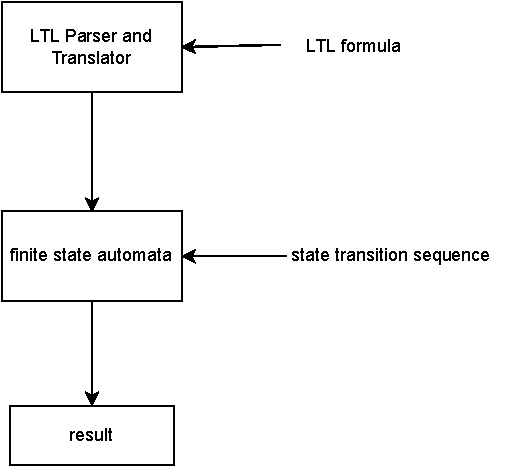
\includegraphics[width=0.9\textwidth]{./figs/translator}
\caption{LTL Checker}
\label{fig:translator}
\end{figure*}

以下为基于该框架的LTL检查算法:
\begin{algorithm} % This algorithm can also be used
\caption{LTL Checker}\label{checker}
\begin{algorithmic}[1]
\STATE input:$(\rho, o)$
\STATE $l \gets getLTL(o)$
\STATE $\alpha \gets transform(l)$ \COMMENT{transform LTL to automaton}
\FOR{$i \leftarrow 0, len(\rho)-1$}
  \STATE $s \gets si(\rho, i)$
  \IF {$\alpha.isTransitable(s)$}
    \STATE $\alpha.transit(s)$
    \ELSE
    \STATE $trigger(o)$
  \ENDIF
\ENDFOR
\IF {$o$ is an achievement goal and $\alpha$ is in final state}
  \STATE $o.achieved()$
\ENDIF
\end{algorithmic}
\end{algorithm}
该检查器的输入参数有两个:游程$\rho$和一个LTL对象$o$。
%
% @TODO: line number ref.
检查器首先得到LTL公式并将其转化为状态机。然后$\rho$中的每个状态都由状态机迭代处理并根据每个环境状态进行状态机的状态转移\footnote{注意,环境状态与状态机中的状态是两个不同的概念。};如果状态机可在当前环境状态下进行转换,则应用该转换。否则,状态机不接收当前环境状态,其相应LTL对象被触发。对于维持型目标,出发意味着维持条件不满足,智能体此时应执行相关修复计划;对于norm,触发意味着norm被触发且智能体收到相应的价值;最后,如果该LTL公式对应一个实现型目标,并且状态机处于其最终状态(Final State),那么该目标被视为已实现。

算法\ref{trigger}所示的触发函数用于对触发LTL对象的相应操作。
\begin{algorithm} % This algorithm can also be used
\caption{trigger function}\label{trigger}
\begin{algorithmic}[1]
\STATE input:$(o)$

\IF {$o$ is a maintenance goal and no recover plan is adopted}
\STATE adopt a recover plan
\ELSE
\IF {$o$ is a norm}
\STATE receive value $o.Val$
\ENDIF
\ENDIF

\end{algorithmic}
\end{algorithm}

在描述对\SA 法的修改之前,本节首先描述智能体的初始设定以及骑在执行期间的内部状态转换规则:假设智能体在开始执行时被分配了一组需要满足的LTL公式,在正式执行之前,智能体首先将每个LTL公式转化为状态机(状态机为智能体内部状态的一部分);在智能体执行过程中,每次更新智能体信念集合时,所有状态机都会根据智能体当前对环境的认知进行状态转移;如果在当前认知下,状态机中可由可应用的状态转移规则,则按照算法\ref{checker}所述触发其相关操作。

\subsection{对\SA 法的修改}
为了支持LTL表示形式下的意图调度,\SAT 修改了\SA 算法中的扩展与模拟阶段,具体修改如下:
\paragraph{对扩展阶段的修改}
% Reactive
在扩展阶段,\SAT 首先检查某个选中的叶子节点$n_s$状态下每一个可执行动作$a_i$,若$a_i$所引发的(状态机的)状态转移不会使得智能体获得负收益,则直接生成一个新的节点对应于执行$a_i$的结果,并作为$N_s$的一个孩子节点。若$a_i$会引发负收益,则首先进行如下检查:检查$a_i$所对应的状态机$m_i$,若$m_i$可获得的最终的价值$V_i$大于当前执行$m_i$相关动作所受到的总惩罚值$P_i$(包括执行$a_i$的惩罚值),则生成一个新节点对应于执行$a_i$的结果。相反,若$m_i$可获得的最终价值$V_i$小于当前执行$m_i$相关动作所受到的总惩罚值$P_i$,则不生成新的节点。
%
当所有可执行动作$a_i$都会造成$P_i > V_i$时,则不会有新的节点生成。该情况下智能体会暂停其执行。
%
在\SAT 中,每个节点记录的信息除智能体意图、环境状态外,还记录了执行过程中所收到的总价值(收益值以及惩罚值)和每个状态机单独得到的价值。

\paragraph{对模拟阶段的修改}
在模拟阶段,\SAT 和\SA 一样,随机选择实现目标过程中可执行的动作执行。当某个可执行动作$a_i$造成状态机的状态转移并获得负收益时时,进行如下检查:检查$a_i$对应的状态机$m_i$,若可获得的最终的价值$V_i$大于当前执行$m_i$相关动作所受到的总惩罚值$P_i$(包括执行$a_i$的惩罚值),则禁止该动作的执行。相反,若$m_i$可获得的最终价值$V_i$小于当前执行$m_i$相关动作所受到的总惩罚值$P_i$,则直接执行。

当以下三个条件中的任意一个满足时,模拟阶段即停止:
\begin{enumerate}
  \item 所有状态机都处于最终状态。
  \item 并非所有状态机都处于最终状态,但是智能体无法执行相关动作将其带入最终状态。
  \item 所有的可执行动作$a_i$都会导致$m_i$可获得的最终价值$V_i$小于当前执行$m_i$相关动作所受到的总惩罚值$P_i$。
\end{enumerate}

\section{实验}
本章的实验场景与上一章类似,基于火星探测器的模拟场景(见图\ref{fig:marsrover})。不同的是同时考虑到了维持型目标和norm的情况。维持型目标与norm的相关场景设定与第\ref{mg}和第\ref{norm}相同,在此不再赘述。

% measring the agent performance
本实验根据三个指标对智能体的性能进行评估:完成目标的数量、电池消耗量以及总惩罚值。具体地,本实验根据评估函数$\frac{\#goals}{batteryConsumption} - penaltyValue$对智能体的性能进行评估,其中$\#goals$为实现目标的数量,$batteryConsumption$为电池消耗量,$penaltyValue$为因违反norm而受到的总惩罚值。该价值函数决定了智能体的综合性能表现。

本文将\SAN 与Duff等人\cite{DBLP:conf/atal/DuffHT06}提出的PMG(本章对RMG也进行了实验,其作为基准以衡量其他方法的性能)和Meneguzzi等人\cite{DBLP:journals/eaai/MeneguzziROVL15}提出的v-BDI进行比较。PMG和v-BDI算法分别在第\ref{mg}章和第\ref{norm}章有所解释,在此不再赘述。

在接下来的实验中,v-BDI的价值函数被设定为$\frac{\#goals}{batteryConsumption} - penaltyValue$。\SAN 算法设定为执行100次迭代($\alpha = 100$),每次迭代执行10次的模拟($\beta = 10$)。\SAN 的价值函数与v-BDI相同,设定为$\frac{\#goals}{batteryConsumption} - penaltyValue$。

\subsection{低电池容量实验}
以下实验中考虑智能体在低电池容量下设定的性能表现。在低电池容量设定下,智能体的电池容量被设定为40。具体实验结果如图\ref{}所示。

\paragraph{惩罚值分析}
如图所示,随着norm数量的增加,所有智能体受到的惩罚值也相应增加。RMG受到的惩罚值最大。其原因有三部分:
\begin{enumerate}
  \item RMG缺乏对norm的处理能力,所有违反norm的行为都被RMG所忽略;
  \item 其次,由于其意图调度策略的设定(FIFO规则),RMG没有考虑到多个意图间的交互,使得其在地图中的移动距离更长,这可能导致更多的norm违反情况发生;
  \item 最后,RMG以被动方式处理维持型目标,这也会导致其在地图中的移动距离更长。
\end{enumerate}
与NMG相比,PMG具有更好的性能表现,这是由于其主动性的应对维持目标策略:若实现下一个目标会破坏维持条件,智能体将首先返回基地充电再考虑实现目标。这种策略节省了很多执行步骤,从而减少了执行过程中违反norm的次数。v-BDI比NMG有更好的性能表现,因为其可以在计划选择阶段考虑避免对norm的违反,减少了norm的违反次数。
\paragraph{电量消耗分析}
虽然所有方法的电量消耗都随着目标数量的增加而增加,但是RMG和PMG的电量消耗并不会随着norm数量的增加而改变(当目标数量相同情况下)。这是因为norm并不会改变RMG和PMG实现目标的顺序和方式。尽管v-BDI在电量消耗方面与RMG有着几乎相同的性能表现,但是随着norm数量的增加,其电量消耗有一定微小变化。这是因为norm确实会影响其计划选择,这可能会影响智能体是否会意外实现其他目标,而意外实现其他目标最终会有节省电量的效果,导致与RMG有微小差异。从该图中可得到的一个重要信息是当norm数量增加时,MCTS消耗的电量有所增加。这是由于其效用函数的设置$\frac{\#goals}{batteryConsumption} - penaltyValue$,当norm的数量较多时,MCTS讲牺牲其利用多意图间协同效应的能力,以更好的避免违反norm。最后,相比于其他方法,MCTS仍然有着最优秀的性能表现。
\paragraph{总价值分析}
随着norm数量的增加,所有方法的总价值都相应降低。MCTS的性能明显优于其他方法。在norm的数量为10的情况下,当目标数量增加时,MCTS的性能只有略微下降。这是因为由于目标数量的增加,MCTS可以更好地利用多意图间的协同效应,因此,协同效应带来的优势克服了违反norm次数增加造成的危害,从而获得较高的总价值。然而,正如图中所示,当norm的数量较多时,违反norm的危害难以得到补偿。

\subsection{高电池容量实验}
以下实验中考虑智能体在高电池容量下设定的性能表现。在高电池容量设定下,智能体的电池容量被设定为120。具体实验结果如图\ref{}所示。

在高电池容量设定下,这四种方法的性能变化趋势与低电池容量实验相似。明显不同之处在于,高电池容量下各个方法的性能表现相较于低电池容量都有所增加。
\paragraph{惩罚值分析}
在惩罚值方面,RMG和PMG之间的差异比低电池容量下小很多。这是因为高电池容量下智能体有相对充足的电量一次执行多个任务,维持型目标被触发的可能性和次数降低,这造成主动和被动的维持型目标直接差异无法很好得到体现。然而v-BDI受益于其考虑norm的计划选择策略,其性能相比于RMG和PMG仍有较为明显的优势。最后,正如所预料的,MCTS拥有最好的性能表现。
\paragraph{电量消耗分析}
RMG、PMG和v-BDI在电量消耗方面具有几乎相同的性能,这同样也是因为在高电池容量下智能体很少触发维持型目标,使得这些方法最终的行为表现很类似,消耗的电量非常相近。
\paragraph{总价值分析}
RMG和PMG在总价值方面同样也具有几乎相同的性能表现。然而尽管与RMG和PMG相比,v-BDI在消耗电量方面并无优势,但其总价值却比RMG和PMG高很多。这是因为与RMG和PMG相比,v-BDI受到的惩罚值更低,导致最终的总价值更高。最后,由于同时考虑维持型目标、norm以及利用多意图间协同效应的能力,MCTS的性能表现相较于其他方法有着显著优势。

\section{本章总结}
本章提出了一种基于MCTS的意图调度算法\SAT 。\SAT 可以在norm约束下同时对智能体的实现型目标和维持型目标进行意图调度。另外,基于火星探测器的模拟场景,本章在迪电池容量以及高电池容量场景下对\SAT 的性能进行了分析。实验结果表明\SAT 与其他方法(PMG和v-BDI)相比有着显著的性能优势。

\chapter{结论与未来展望}
\section{结论}
\section{展望}





%% % !TeX root = ../thuthesis-example.tex

\chapter{论文主要部分的写法}

研究生学位论文撰写,除表达形式上需要符合一定的格式要求外,内容方面上也要遵循一些共性原则。

通常研究生学位论文只能有一个主题(不能是几块工作拼凑在一起),该主题应针对某学科领域中的一个具体问题展开深入、系统的研究,并得出有价值的研究结论。
学位论文的研究主题切忌过大,例如,“中国国有企业改制问题研究”这样的研究主题过大,因为“国企改制”涉及的问题范围太广,很难在一本研究生学位论文中完全研究透彻。



\section{论文的语言及表述}

除国际研究生外,学位论文一律须用汉语书写。
学位论文应当用规范汉字进行撰写,除古汉语研究中涉及的古文字和参考文献中引用的外文文献之外,均采用简体汉字撰写。

国际研究生一般应以中文或英文书写学位论文,格式要求同上。
论文须用中文封面。

研究生学位论文是学术作品,因此其表述要严谨简明,重点突出,专业常识应简写或不写,做到立论正确、数据可靠、说明透彻、推理严谨、文字凝练、层次分明,避免使用文学性质的或带感情色彩的非学术性语言。

论文中如出现一个非通用性的新名词、新术语或新概念,需随即解释清楚。



\section{论文题目的写法}

论文题目应简明扼要地反映论文工作的主要内容,力求精炼、准确,切忌笼统。
论文题目是对研究对象的准确、具体描述,一般要在一定程度上体现研究结论,因此,论文题目不仅应告诉读者这本论文研究了什么问题,更要告诉读者这个研究得出的结论。
例如:“在事实与虚构之间:梅乐、卡彭特、沃尔夫的新闻观”就比“三个美国作家的新闻观研究”更专业、更准确。



\section{摘要的写法}

论文摘要是对论文研究内容的高度概括,应具有独立性和自含性,即应是 一篇简短但意义完整的文章。
通过阅读论文摘要,读者应该能够对论文的研究 方法及结论有一个整体性的了解,因此摘要的写法应力求精确简明。
论文摘要 应包括对问题及研究目的的描述、对使用的方法和研究过程进行的简要介绍、 对研究结论的高度凝练等,重点是结果和结论。

论文摘要切忌写成全文的提纲,尤其要避免“第 1 章……;第 2 章……;……”这样的陈述方式。



\section{引言的写法}

一篇学位论文的引言大致包含如下几个部分:
1、问题的提出;
2、选题背 景及意义;
3、文献综述;
4、研究方法;
5、论文结构安排。
\begin{itemize}
  \item 问题的提出:要清晰地阐述所要研究的问题“是什么”。
    \footnote{选题时切记要有“问题意识”,不要选不是问题的问题来研究。}
  \item 选题背景及意义:论述清楚为什么选择这个题目来研究,即阐述该研究对学科发展的贡献、对国计民生的理论与现实意义等。
  \item 文献综述:对本研究主题范围内的文献进行详尽的综合述评,“述”的同时一定要有“评”,指出现有研究状态,仍存在哪些尚待解决的问题,讲出自己的研究有哪些探索性内容。
  \item 研究方法:讲清论文所使用的学术研究方法。
  \item 论文结构安排:介绍本论文的写作结构安排。
\end{itemize}



\section{正文的写法}

本部分是论文作者的研究内容,不能将他人研究成果不加区分地掺和进来。
已经在引言的文献综述部分讲过的内容,这里不需要再重复。
各章之间要存在有机联系,符合逻辑顺序。



\section{结论的写法}

结论是对论文主要研究结果、论点的提炼与概括,应精炼、准确、完整,使读者看后能全面了解论文的意义、目的和工作内容。
结论是最终的、总体的结论,不是正文各章小结的简单重复。
结论应包括论文的核心观点,主要阐述作者的创造性工作及所取得的研究成果在本领域中的地位、作用和意义,交代研究工作的局限,提出未来工作的意见或建议。
同时,要严格区分自己取得的成果与指导教师及他人的学术成果。

在评价自己的研究工作成果时,要实事求是,除非有足够的证据表明自己的研究是“首次”、“领先”、“填补空白”的,否则应避免使用这些或类似词语。

%% % !TeX root = ../thuthesis-example.tex

\chapter{图表示例}

\section{插图}

图片通常在 \env{figure} 环境中使用 \cs{includegraphics} 插入,如图~\ref{fig:example} 的源代码。
建议矢量图片使用 PDF 格式,比如数据可视化的绘图;
照片应使用 JPG 格式;
其他的栅格图应使用无损的 PNG 格式。
注意,LaTeX 不支持 TIFF 格式;EPS 格式已经过时。

\begin{figure}
  \centering
  \includegraphics[width=0.5\linewidth]{example-image-a.pdf}
  \caption*{国外的期刊习惯将图表的标题和说明文字写成一段,需要改写为标题只含图表的名称,其他说明文字以注释方式写在图表下方,或者写在正文中。}
  \caption{示例图片标题}
  \label{fig:example}
\end{figure}

若图或表中有附注,采用英文小写字母顺序编号,附注写在图或表的下方。
国外的期刊习惯将图表的标题和说明文字写成一段,需要改写为标题只含图表的名称,其他说明文字以注释方式写在图表下方,或者写在正文中。

如果一个图由两个或两个以上分图组成时,各分图分别以 (a)、(b)、(c)...... 作为图序,并须有分图题。
推荐使用 \pkg{subcaption} 宏包来处理, 比如图~\ref{fig:subfig-a} 和图~\ref{fig:subfig-b}。

\begin{figure}
  \centering
  \subcaptionbox{分图 A\label{fig:subfig-a}}
    {\includegraphics[width=0.35\linewidth]{example-image-a.pdf}}
  \subcaptionbox{分图 B\label{fig:subfig-b}}
    {\includegraphics[width=0.35\linewidth]{example-image-b.pdf}}
  \caption{多个分图的示例}
  \label{fig:multi-image}
\end{figure}



\section{表格}

表应具有自明性。为使表格简洁易读,尽可能采用三线表,如表~\ref{tab:three-line}。
三条线可以使用 \pkg{booktabs} 宏包提供的命令生成。

\begin{table}
  \centering
  \caption{三线表示例}
  \begin{tabular}{ll}
    \toprule
    文件名          & 描述                         \\
    \midrule
    thuthesis.dtx   & 模板的源文件,包括文档和注释 \\
    thuthesis.cls   & 模板文件                     \\
    thuthesis-*.bst & BibTeX 参考文献表样式文件    \\
    \bottomrule
  \end{tabular}
  \label{tab:three-line}
\end{table}

表格如果有附注,尤其是需要在表格中进行标注时,可以使用 \pkg{threeparttable} 宏包。
研究生要求使用英文小写字母 a、b、c……顺序编号,本科生使用圈码 ①、②、③……编号。

\begin{table}
  \centering
  \begin{threeparttable}[c]
    \caption{带附注的表格示例}
    \label{tab:three-part-table}
    \begin{tabular}{ll}
      \toprule
      文件名                 & 描述                         \\
      \midrule
      thuthesis.dtx\tnote{a} & 模板的源文件,包括文档和注释 \\
      thuthesis.cls\tnote{b} & 模板文件                     \\
      thuthesis-*.bst        & BibTeX 参考文献表样式文件    \\
      \bottomrule
    \end{tabular}
    \begin{tablenotes}
      \item [a] 可以通过 xelatex 编译生成模板的使用说明文档;
        使用 xetex 编译 \file{thuthesis.ins} 时则会从 \file{.dtx} 中去除掉文档和注释,得到精简的 \file{.cls} 文件。
      \item [b] 更新模板时,一定要记得编译生成 \file{.cls} 文件,否则编译论文时载入的依然是旧版的模板。
    \end{tablenotes}
  \end{threeparttable}
\end{table}

如某个表需要转页接排,可以使用 \pkg{longtable} 宏包,需要在随后的各页上重复表的编号。
编号后跟表题(可省略)和“(续)”,置于表上方。续表均应重复表头。

\begin{longtable}{cccc}
    \caption{跨页长表格的表题}
    \label{tab:longtable} \\
    \toprule
    表头 1 & 表头 2 & 表头 3 & 表头 4 \\
    \midrule
  \endfirsthead
    \caption*{续表~\thetable\quad 跨页长表格的表题} \\
    \toprule
    表头 1 & 表头 2 & 表头 3 & 表头 4 \\
    \midrule
  \endhead
    \bottomrule
  \endfoot
  Row 1  & & & \\
  Row 2  & & & \\
  Row 3  & & & \\
  Row 4  & & & \\
  Row 5  & & & \\
  Row 6  & & & \\
  Row 7  & & & \\
  Row 8  & & & \\
  Row 9  & & & \\
  Row 10 & & & \\
\end{longtable}



\section{算法}

算法环境可以使用 \pkg{algorithms} 或者 \pkg{algorithm2e} 宏包。

\renewcommand{\algorithmicrequire}{\textbf{输入:}\unskip}
\renewcommand{\algorithmicensure}{\textbf{输出:}\unskip}

\begin{algorithm}
  \caption{Calculate $y = x^n$}
  \label{alg1}
  \small
  \begin{algorithmic}
    \REQUIRE $n \geq 0$
    \ENSURE $y = x^n$

    \STATE $y \leftarrow 1$
    \STATE $X \leftarrow x$
    \STATE $N \leftarrow n$

    \WHILE{$N \neq 0$}
      \IF{$N$ is even}
        \STATE $X \leftarrow X \times X$
        \STATE $N \leftarrow N / 2$
      \ELSE[$N$ is odd]
        \STATE $y \leftarrow y \times X$
        \STATE $N \leftarrow N - 1$
      \ENDIF
    \ENDWHILE
  \end{algorithmic}
\end{algorithm}

%% % !TeX root = ../thuthesis-example.tex

\chapter{数学符号和公式}

\section{数学符号}

中文论文的数学符号默认遵循 GB/T 3102.11—1993《物理科学和技术中使用的数学符号》
\footnote{原 GB 3102.11—1993,自 2017 年 3 月 23 日起,该标准转为推荐性标准。}。
该标准参照采纳 ISO 31-11:1992 \footnote{目前已更新为 ISO 80000-2:2019。},
但是与 \TeX{} 默认的美国数学学会(AMS)的符号习惯有所区别。
具体地来说主要有以下差异:
\begin{enumerate}
  \item 大写希腊字母默认为斜体,如
    \begin{equation*}
      \Gamma \Delta \Theta \Lambda \Xi \Pi \Sigma \Upsilon \Phi \Psi \Omega.
    \end{equation*}
    注意有限增量符号 $\increment$ 固定使用正体,模板提供了 \cs{increment} 命令。
  \item 小于等于号和大于等于号使用倾斜的字形 $\le$、$\ge$。
  \item 积分号使用正体,比如 $\int$、$\oint$。
  \item
    偏微分符号 $\partial$ 使用正体。
  \item
    省略号 \cs{dots} 按照中文的习惯固定居中,比如
    \begin{equation*}
      1, 2, \dots, n \quad 1 + 2 + \dots + n.
    \end{equation*}
  \item
    实部 $\Re$ 和虚部 $\Im$ 的字体使用罗马体。
\end{enumerate}

以上数学符号样式的差异可以在模板中统一设置。
另外国标还有一些与 AMS 不同的符号使用习惯,需要用户在写作时进行处理:
\begin{enumerate}
  \item 数学常数和特殊函数名用正体,如
    \begin{equation*}
      \uppi = 3.14\dots; \quad
      \symup{i}^2 = -1; \quad
      \symup{e} = \lim_{n \to \infty} \left( 1 + \frac{1}{n} \right)^n.
    \end{equation*}
  \item 微分号使用正体,比如 $\dif y / \dif x$。
  \item 向量、矩阵和张量用粗斜体(\cs{symbf}),如 $\symbf{x}$、$\symbf{\Sigma}$、$\symbfsf{T}$。
  \item 自然对数用 $\ln x$ 不用 $\log x$。
\end{enumerate}


英文论文的数学符号使用 \TeX{} 默认的样式。
如果有必要,也可以通过设置 \verb|math-style| 选择数学符号样式。

关于量和单位推荐使用
\href{http://mirrors.ctan.org/macros/latex/contrib/siunitx/siunitx.pdf}{\pkg{siunitx}}
宏包,
可以方便地处理希腊字母以及数字与单位之间的空白,
比如:
\SI{6.4e6}{m},
\SI{9}{\micro\meter},
\si{kg.m.s^{-1}},
\SIrange{10}{20}{\degreeCelsius}。



\section{数学公式}

数学公式可以使用 \env{equation} 和 \env{equation*} 环境。
注意数学公式的引用应前后带括号,通常使用 \cs{eqref} 命令,比如式\eqref{eq:example}。
\begin{equation}
  \frac{1}{2 \uppi \symup{i}} \int_\gamma f = \sum_{k=1}^m n(\gamma; a_k) \mathscr{R}(f; a_k).
  \label{eq:example}
\end{equation}

多行公式尽可能在“=”处对齐,推荐使用 \env{align} 环境。
\begin{align}
  a & = b + c + d + e \\
    & = f + g
\end{align}



\section{数学定理}

定理环境的格式可以使用 \pkg{amsthm} 或者 \pkg{ntheorem} 宏包配置。
用户在导言区载入这两者之一后,模板会自动配置 \env{thoerem}、\env{proof} 等环境。

\begin{theorem}[Lindeberg--Lévy 中心极限定理]
  设随机变量 $X_1, X_2, \dots, X_n$ 独立同分布, 且具有期望 $\mu$ 和有限的方差 $\sigma^2 \ne 0$,
  记 $\bar{X}_n = \frac{1}{n} \sum_{i+1}^n X_i$,则
  \begin{equation}
    \lim_{n \to \infty} P \left(\frac{\sqrt{n} \left( \bar{X}_n - \mu \right)}{\sigma} \le z \right) = \Phi(z),
  \end{equation}
  其中 $\Phi(z)$ 是标准正态分布的分布函数。
\end{theorem}
\begin{proof}
  Trivial.
\end{proof}

同时模板还提供了 \env{assumption}、\env{definition}、\env{proposition}、
\env{lemma}、\env{theorem}、\env{axiom}、\env{corollary}、\env{exercise}、
\env{example}、\env{remar}、\env{problem}、\env{conjecture} 这些相关的环境。

%% % !TeX root = ../thuthesis-example.tex

\chapter{引用文献的标注}

模板支持 BibTeX 和 BibLaTeX 两种方式处理参考文献。
下文主要介绍 BibTeX 配合 \pkg{natbib} 宏包的主要使用方法。


\section{顺序编码制}

在顺序编码制下,默认的 \cs{cite} 命令同 \cs{citep} 一样,序号置于方括号中,
引文页码会放在括号外。
统一处引用的连续序号会自动用短横线连接。

\thusetup{
  cite-style = super,
}
\begin{tabular}{l@{\quad$\Rightarrow$\quad}l}
  \verb|\cite{zhangkun1994}|               & \cite{zhangkun1994}               \\
  \verb|\citet{zhangkun1994}|              & \citet{zhangkun1994}              \\
  \verb|\citep{zhangkun1994}|              & \citep{zhangkun1994}              \\
  \verb|\cite[42]{zhangkun1994}|           & \cite[42]{zhangkun1994}           \\
  \verb|\cite{zhangkun1994,zhukezhen1973}| & \cite{zhangkun1994,zhukezhen1973} \\
\end{tabular}


也可以取消上标格式,将数字序号作为文字的一部分。
建议全文统一使用相同的格式。

\thusetup{
  cite-style = inline,
}
\begin{tabular}{l@{\quad$\Rightarrow$\quad}l}
  \verb|\cite{zhangkun1994}|               & \cite{zhangkun1994}               \\
  \verb|\citet{zhangkun1994}|              & \citet{zhangkun1994}              \\
  \verb|\citep{zhangkun1994}|              & \citep{zhangkun1994}              \\
  \verb|\cite[42]{zhangkun1994}|           & \cite[42]{zhangkun1994}           \\
  \verb|\cite{zhangkun1994,zhukezhen1973}| & \cite{zhangkun1994,zhukezhen1973} \\
\end{tabular}



\section{著者-出版年制}

著者-出版年制下的 \cs{cite} 跟 \cs{citet} 一样。

\thusetup{
  cite-style = author-year,
}
\begin{tabular}{l@{\space$\Rightarrow$\space}l}
  \verb|\cite{zhangkun1994}|                & \cite{zhangkun1994}                \\
  \verb|\citet{zhangkun1994}|               & \citet{zhangkun1994}               \\
  \verb|\citep{zhangkun1994}|               & \citep{zhangkun1994}               \\
  \verb|\cite[42]{zhangkun1994}|            & \cite[42]{zhangkun1994}            \\
  \verb|\citep{zhangkun1994,zhukezhen1973}| & \citep{zhangkun1994,zhukezhen1973} \\
\end{tabular}

\vskip 2ex
\thusetup{
  cite-style = super,
}
注意,引文参考文献的每条都要在正文中标注
\cite{zhangkun1994,zhukezhen1973,dupont1974bone,zhengkaiqing1987,%
  jiangxizhou1980,jianduju1994,merkt1995rotational,mellinger1996laser,%
  bixon1996dynamics,mahui1995,carlson1981two,taylor1983scanning,%
  taylor1981study,shimizu1983laser,atkinson1982experimental,%
  kusch1975perturbations,guangxi1993,huosini1989guwu,wangfuzhi1865songlun,%
  zhaoyaodong1998xinshidai,biaozhunhua2002tushu,chubanzhuanye2004,%
  who1970factors,peebles2001probability,baishunong1998zhiwu,%
  weinstein1974pathogenic,hanjiren1985lun,dizhi1936dizhi,%
  tushuguan1957tushuguanxue,aaas1883science,fugang2000fengsha,%
  xiaoyu2001chubanye,oclc2000about,scitor2000project%
}。



% 其他部分
\backmatter

% 参考文献
\bibliography{bibliography}  % 参考文献使用 BibTeX 编译
% \bibliography{ref/refs}  % 参考文献使用 BibTeX 编译
% \printbibliography       % 参考文献使用 BibLaTeX 编译

% 附录
% 本科生需要将附录放到声明之后,个人简历之前
%% \appendix
% % !TeX root = ../thuthesis-example.tex

\begin{survey}
\label{cha:survey}

\title{Title of the Survey}
\maketitle


\tableofcontents


本科生的外文资料调研阅读报告。


\section{Figures and Tables}

\subsection{Figures}

An example figure in appendix (Figure~\ref{fig:appendix-survey-figure}).

\begin{figure}
  \centering
  \includegraphics[width=0.6\linewidth]{example-image-a.pdf}
  \caption{Example figure in appendix}
  \label{fig:appendix-survey-figure}
\end{figure}


\subsection{Tables}

An example table in appendix (Table~\ref{tab:appendix-survey-table}).

\begin{table}
  \centering
  \caption{Example table in appendix}
  \begin{tabular}{ll}
    \toprule
    File name       & Description                                         \\
    \midrule
    thuthesis.dtx   & The source file including documentaion and comments \\
    thuthesis.cls   & The template file                                   \\
    thuthesis-*.bst & BibTeX styles                                       \\
    thuthesis-*.bbx & BibLaTeX styles for bibliographies                  \\
    thuthesis-*.cbx & BibLaTeX styles for citations                       \\
    \bottomrule
  \end{tabular}
  \label{tab:appendix-survey-table}
\end{table}


\section{Equations}

An example equation in appendix (Equation~\eqref{eq:appendix-survey-equation}).
\begin{equation}
  \frac{1}{2 \uppi \symup{i}} \int_\gamma f = \sum_{k=1}^m n(\gamma; a_k) \mathscr{R}(f; a_k)
  \label{eq:appendix-survey-equation}
\end{equation}


\section{Citations}

Example citations in appendix.
\cite{abrahams99tex}
\cite{salomon1995advanced}
\cite{abrahams99tex,salomon1995advanced}


\bibliographystyle{unsrtnat}
\bibliography{ref/appendix}

\end{survey}
       % 本科生:外文资料的调研阅读报告
% % !TeX root = ../thuthesis-example.tex

\begin{translation}
\label{cha:translation}

\title{书面翻译题目}
\maketitle

\tableofcontents


本科生的外文资料书面翻译。


\section{图表示例}

\subsection{图}

附录中的图片示例(图~\ref{fig:appendix-translation-figure})。

\begin{figure}
  \centering
  \includegraphics[width=0.6\linewidth]{example-image-a.pdf}
  \caption{附录中的图片示例}
  \label{fig:appendix-translation-figure}
\end{figure}


\subsection{表格}

附录中的表格示例(表~\ref{tab:appendix-translation-table})。

\begin{table}
  \centering
  \caption{附录中的表格示例}
  \begin{tabular}{ll}
    \toprule
    文件名          & 描述                         \\
    \midrule
    thuthesis.dtx   & 模板的源文件,包括文档和注释 \\
    thuthesis.cls   & 模板文件                     \\
    thuthesis-*.bst & BibTeX 参考文献表样式文件    \\
    thuthesis-*.bbx & BibLaTeX 参考文献表样式文件  \\
    thuthesis-*.cbx & BibLaTeX 引用样式文件        \\
    \bottomrule
  \end{tabular}
  \label{tab:appendix-translation-table}
\end{table}


\section{数学公式}

附录中的数学公式示例(公式\eqref{eq:appendix-translation-equation})。
\begin{equation}
  \frac{1}{2 \uppi \symup{i}} \int_\gamma f = \sum_{k=1}^m n(\gamma; a_k) \mathscr{R}(f; a_k)
  \label{eq:appendix-translation-equation}
\end{equation}


\section{文献引用}

文献引用示例\cite{abrahams99tex}。


\appendix

\section{附录}

附录的内容。


% 书面翻译的参考文献
\bibliographystyle{unsrtnat}
\bibliography{ref/appendix}

% 书面翻译对应的原文索引
\begin{translation-index}
  \nocite{salomon1995advanced}
  \bibliographystyle{unsrtnat}
  \bibliography{ref/appendix}
\end{translation-index}

\end{translation}
  % 本科生:外文资料的书面翻译
%% % !TeX root = ../thuthesis-example.tex

\chapter{补充内容}

附录是与论文内容密切相关、但编入正文又影响整篇论文编排的条理和逻辑性的资料,例如某些重要的数据表格、计算程序、统计表等,是论文主体的补充内容,可根据需要设置。


\section{图表示例}

\subsection{图}

附录中的图片示例(图~\ref{fig:appendix-figure})。

\begin{figure}
  \centering
  \includegraphics[width=0.6\linewidth]{example-image-a.pdf}
  \caption{附录中的图片示例}
  \label{fig:appendix-figure}
\end{figure}


\subsection{表格}

附录中的表格示例(表~\ref{tab:appendix-table})。

\begin{table}
  \centering
  \caption{附录中的表格示例}
  \begin{tabular}{ll}
    \toprule
    文件名          & 描述                         \\
    \midrule
    thuthesis.dtx   & 模板的源文件,包括文档和注释 \\
    thuthesis.cls   & 模板文件                     \\
    thuthesis-*.bst & BibTeX 参考文献表样式文件    \\
    thuthesis-*.bbx & BibLaTeX 参考文献表样式文件  \\
    thuthesis-*.cbx & BibLaTeX 引用样式文件        \\
    \bottomrule
  \end{tabular}
  \label{tab:appendix-table}
\end{table}


\section{数学公式}

附录中的数学公式示例(公式\eqref{eq:appendix-equation})。
\begin{equation}
  \frac{1}{2 \uppi \symup{i}} \int_\gamma f = \sum_{k=1}^m n(\gamma; a_k) \mathscr{R}(f; a_k)
  \label{eq:appendix-equation}
\end{equation}


% 致谢
% % !TeX root = ../thuthesis-example.tex

\begin{acknowledgements}
  衷心感谢导师×××教授和物理系××副教授对本人的精心指导。他们的言传身教将使我终生受益。

  在美国麻省理工学院化学系进行九个月的合作研究期间,承蒙 Robert Field 教授热心指导与帮助,不胜感激。

  感谢×××××实验室主任×××教授,以及实验室全体老师和同窗们学的热情帮助和支持!

  本课题承蒙国家自然科学基金资助,特此致谢。
\end{acknowledgements}


% 声明
% \statement
% 将签字扫描后的声明文件 scan-statement.pdf 替换原始页面
% \statement[file=scan-statement.pdf]
% 本科生编译生成的声明页默认不加页脚,插入扫描版时再补上;
% 研究生编译生成时有页眉页脚,插入扫描版时不再重复。
% 也可以手动控制是否加页眉页脚
% \statement[page-style=empty]
% \statement[file=scan-statement.pdf, page-style=plain]

% 个人简历、在学期间完成的相关学术成果
% 本科生可以附个人简历,也可以不附个人简历
% !TeX root = ../thuthesis-example.tex

\begin{resume}

  \section*{个人简历}

  1998 年 7 月 出生于江西鹰潭。

  2020 年 9 月 -- 2023 年 6 月,浙江工业大学计算机学院软件工程专业学习,攻读工学硕士学位。


  \section*{在学期间完成的相关学术成果}

  \subsection*{学术论文}

  \begin{achievements}
    \item Yuan Y, Di W.Engineering Multi-Agent Systems - 9th International Workshop, {EMAS}
    2021, accepted.
  \end{achievements}


  \subsection*{专利}

  \begin{achievements}
    \item 姚远, 吴迪, 等. 一种结构化表示智能体目标实现过程的方法. 中国, CN1602118A[P]. 2021-08-13.
    \item 姚远, 吴迪, 等. 一种基于控制变量合成随机目标计划树的方法. 中国, CN114330725A[P]. 2022-04-12.
  \end{achievements}

  \subsection*{软著}
  \begin{achievements}
  \item 姚远, 蔡琰, 吴迪, 等. 目标计划树合成软件. 中国, 登记号:2022SR0251949. 2022-02-21.
  \end{achievements}

\end{resume}


% 指导教师/指导小组评语
% 本科生不需要
% % !TeX root = ../thuthesis-example.tex

\begin{comments}
% \begin{comments}[name = {指导小组评语}]
% \begin{comments}[name = {Comments from Thesis Supervisor}]
% \begin{comments}[name = {Comments from Thesis Supervision Committee}]

  论文提出了……

\end{comments}


% 答辩委员会决议书
% 本科生不需要
% % !TeX root = ../thuthesis-example.tex

\begin{resolution}

  论文提出了……

  论文取得的主要创新性成果包括:

  1. ……

  2. ……

  3. ……

  论文工作表明作者在×××××具有×××××知识,具有××××能力,论文××××,答辩××××。

  答辩委员会表决,(×票/一致)同意通过论文答辩,并建议授予×××(姓名)×××(门类)学博士/硕士学位。

\end{resolution}


% 本科生的综合论文训练记录表(扫描版)
% \record{file=scan-record.pdf}

\end{document}
